%%%%%%%%%%%%%%%%%%%%%%%%%%%%%%%%%
% Main File                     %
%%%%%%%%%%%%%%%%%%%%%%%%%%%%%%%%%
%
% This is the main file of your report. It serves as the starting point and controls the overall structure of your document. Unless you want to add or remove a section, there is usually no need to modify this file.

% Customize the content of the main file by including the necessary sections using the \input command. Each section has its own file, which contains the specific content for that section.

%%%%%%%%%%%%%%%%%%%%%%%%%%%%%%%%%

\documentclass[10pt]{article}

%%%%%%%%%%%%%%%%%%%%%%%%%%%%%%
% Preamble of the project    %
%%%%%%%%%%%%%%%%%%%%%%%%%%%%%%
%
% This file contains the preamble of the project, which includes various packages and settings to customize the document layout, formatting, and styling.

% Make sure to include necessary packages for mathematical symbols, graphics, page layout,
% captions, section headings, lists, hyperlinks, tables, bibliography, and other functionalities.
%
% Remember to update the bibliography file, and include any abbreviations or acronyms needed for your project.
%%%%%%%%%%%%%%%%%%%%%%%%%%%%%%


% Packages
\usepackage{amsmath}  % For \text{}, \eqref, align environments
\usepackage{amssymb} % For mathematical symbols
\usepackage{graphicx} % For including graphics in the document
\usepackage{geometry} % For customizing page layout and margins
\usepackage{titling} % For customizing the title
\usepackage{caption, subcaption} % For creating captions and subcaptions
\usepackage{array} % For customizing table column formatting
\usepackage{booktabs} % For enhanced table formatting
\usepackage{hyperref} % For creating hyperlinks within the document
\usepackage{titlesec} % For customizing section headings
\usepackage{enumitem} % For customizing enumerated and itemized lists
\usepackage{float} % For customizing floating objects like figures and tables
\usepackage{tikz} % For creating graphics and diagrams
\usetikzlibrary{positioning, arrows.meta}
\usepackage{changepage} % For making changes to page layout within the document
\usepackage{indentfirst} % For indenting the first paragraph after section headings
\usepackage{xcolor} % For customizing text and background colors
\usepackage[nottoc]{tocbibind} % For including lists in the table of contents
\usepackage{acronym} % For creating a list of abbreviations
\usepackage{setspace} % For adjusting spacing
\usepackage{fontspec} % For customizing font
\usepackage{fancyhdr} % For customizing page headers and footers
\usepackage{ragged2e} % For text alignment
\usepackage[style=ieee]{biblatex} % For IEEE referencing style
\usepackage{listings}  % For source code listings
\usepackage{dirtree}   % For directory trees

% ── Code listing style ───────────────────────────────────────────────────────
\definecolor{lst-bg}{RGB}{248,249,250}
\definecolor{lst-frame}{RGB}{180,190,200}
\definecolor{lst-comment}{RGB}{80,130,80}
\definecolor{lst-keyword}{RGB}{0,90,180}
\definecolor{lst-string}{RGB}{180,60,0}
\definecolor{lst-number}{RGB}{120,120,120}
\definecolor{lst-linenum}{RGB}{150,150,150}

\lstdefinestyle{bakocode}{
  backgroundcolor  = \color{lst-bg},
  basicstyle       = \ttfamily\footnotesize\setstretch{1.0},
  breakatwhitespace= false,
  breaklines       = true,
  captionpos       = b,
  commentstyle     = \color{lst-comment}\itshape,
  keywordstyle     = \color{lst-keyword}\bfseries,
  stringstyle      = \color{lst-string},
  numberstyle      = \tiny\color{lst-linenum},
  numbers          = left,
  numbersep        = 10pt,
  showstringspaces = false,
  tabsize          = 2,
  frame            = single,
  framesep         = 4pt,
  rulecolor        = \color{lst-frame},
  xleftmargin      = 20pt,
  framexleftmargin = 20pt,
  aboveskip        = 10pt,
  belowskip        = 6pt,
  literate         = {->}{{\textrightarrow}}{1}
                     {=>}{{\textrightarrow}}{1},
}

\lstdefinestyle{filetree}{
  backgroundcolor  = \color{lst-bg},
  basicstyle       = \ttfamily\small\setstretch{1.0},
  numbers          = none,
  frame            = single,
  framesep         = 6pt,
  rulecolor        = \color{lst-frame},
  xleftmargin      = 6pt,
  framexleftmargin = 6pt,
  aboveskip        = 8pt,
  belowskip        = 6pt,
  breaklines       = true,
}

% Spacing
\setstretch{1.5}

% Font
\setmainfont{CenturyGothic.ttf}[
    BoldFont=CenturyGothicbold.ttf,
    BoldItalicFont=CGOTHICBI.ttf,
    ItalicFont=gothici.ttf
]

% Titling
\titleformat*{\section}{\fontsize{16pt}{19.2pt}\bfseries\headingfont\MakeUppercase}
\titleformat*{\subsection}{\fontsize{13pt}{15.6pt}\bfseries\headingfont}
\titleformat*{\subsubsection}{\fontsize{13pt}{15.6pt}\bfseries\headingfont}

% Subsubsubsection Command
\newcommand{\subsubsubsection}[1]{%
  \par\addvspace{3.25ex plus 1ex minus .2ex}%
  \noindent{\normalfont\fontsize{12pt}{14pt}\selectfont\bfseries\itshape #1}%
  \par\addvspace{1.5ex plus .2ex}%
}

% Subsubsubsubsection Command
\newcommand{\subsubsubsubsection}[1]{%
  \par\addvspace{3.25ex plus 1ex minus .2ex}%
  \noindent{\normalfont\fontsize{10pt}{12pt}\selectfont\bfseries\itshape #1}%
  \par\addvspace{1.5ex plus .2ex}%
}

% Adjust spacing options
\titlespacing*{\section}{0pt}{2\baselineskip}{0.5\baselineskip}
\titlespacing*{\subsection}{0pt}{1\baselineskip}{0.5\baselineskip}
\titlespacing*{\subsubsection}{0pt}{1\baselineskip}{0.5\baselineskip}
\titlespacing*{\subsubsubsection}{0pt}{1\baselineskip}{0.5\baselineskip}
\titlespacing*{\subsubsubsubsection}{0pt}{1\baselineskip}{0.5\baselineskip}

% Format \section
\titleformat{\section}
{\fontsize{16pt}{19pt}\selectfont\bfseries\MakeUppercase}
{\thesection}
{0.5em}
{}

% Format \subsection
\titleformat{\subsection}
{\fontsize{13pt}{15.6pt}\selectfont\bfseries}
{\thesubsection}
{0.5em}
{}

% Format \subsubsection
\titleformat{\subsubsection}
{\fontsize{13pt}{15.6pt}\selectfont\bfseries}
{\thesubsubsection}
{0.5em}
{}

% Format \subsubsubsection
\titleformat{\subsubsubsection}
{\fontsize{12pt}{14pt}\selectfont\bfseries\itshape}
{}
{0em}
{}

% Format \subsubsubsubsection
\titleformat{\subsubsubsubsection}
{\fontsize{10pt}{12pt}\selectfont\bfseries\itshape}
{}
{0em}
{}

% Margins
\geometry{margin=2.5cm}

% Justification
\justifying

% Widow and orphan prevention
\widowpenalty=10000
\clubpenalty=10000
\displaywidowpenalty=10000

% Pagination
\pagestyle{fancy}
\fancyhf{}
\rfoot{\thepage}
\renewcommand{\headrulewidth}{0pt}
\renewcommand{\footrulewidth}{0pt}

% Set paragraph indentation
\setlength{\parindent}{1.27cm}

% Customize caption format for figures and tables
\captionsetup[figure]{labelfont={bf},textfont={normalfont}}
\captionsetup[table]{labelfont={bf},textfont={normalfont}}

% Change the title of the table of contents
\renewcommand{\contentsname}{Table of Contents}

% Bibliography
\addbibresource{references.bib}

% Include the preamble file, which contains the necessary packages and settings for customizing the document layout and formatting.

\begin{document}

%%%%%%%%%%%%%%%%%%%%%%%%%%%%%%%%%
% Title Page                    %
%%%%%%%%%%%%%%%%%%%%%%%%%%%%%%%%%
%
% This file contains the code for the title page of the project. It includes the necessary elements to create a title page, such as the report title, student name, supervisor names, and institution logos.

% Customize the content of the title page by replacing the placeholders with the actual information of your project, including the logos, report title, student name, supervisor names, institution logos, and the year of the project.

% Make sure to update the file paths of the image files to include the correct location of your project logos.
%%%%%%%%%%%%%%%%%%%%%%%%%%%%%%%%%

% Note: Adjust the vertical spacing throughout the document by modifying the \vspace commands as needed. Increase or decrease the values to achieve the desired spacing elements. Experiment with different values until the spacing meets your requirements. 

\begin{titlepage}
\centering

\includegraphics[width=6cm]{images/MEDTECH-LOGO.png} \hspace{4cm} 
\includegraphics[width=6cm]{images/bakomotorslogo.png}\\
\vspace{0.5cm}
\large{\textbf{COMPUTER SYSTEMS ENGINEERING PROGRAM}}\\
\large{\textbf{ISS 496 --- Senior Project Report}}\\

\vspace{1.2cm}
\textbf{\LARGE{Real-Time Vehicle Monitoring and Diagnostics System}}\\

\vspace{1.2cm}
\Large{\textbf{By:}} \\
\begin{center}
\begin{tabular}{lll}
    Yassine Mtibaa & Mohamed Baccouche & Mahdi Hachicha \\[4pt]
    Hana Gdoura    & Khadija Ben Hamida & Selima Grissa \\[4pt]
    \multicolumn{3}{c}{Fares Smaoui} \\
\end{tabular}
\end{center}

\vspace{0.8cm}
\Large{\textbf{Academic Supervisor:}\\ \ Mortadha DAHMANI} \\

\vspace{0.8cm}
\Large{\textbf{Institution Supervisor:}\\ Achraf ABELLAOUI\\ BAKO Motors}\\

\vspace{1.2cm}
\normalsize{Tunis, 2025 -- 2026}
\end{titlepage}

% Include the titlepage file, which contains the code for the title page of your project.

\pagenumbering{roman}
% Set the page numbering to lowercase Roman numerals for the preliminary sections.


\phantomsection
%%%%%%%%%%%%%%%%%%%%%%%%%%%%%%%%%
% Abstract                      %
%%%%%%%%%%%%%%%%%%%%%%%%%%%%%%%%%

\section*{Abstract}
\addcontentsline{toc}{section}{Abstract}

\vspace{1.4cm}
\large
\noindent

The BAKO Motors Intelligent Supervision System (ISS) is a full-stack embedded IoT platform designed and delivered as part of the ISS~496 senior project at MedTech Mediterranean Institute of Technology, in direct collaboration with BAKO Motors as the industrial partner. The project addresses five critical operational gaps in BAKO Motors' electric vehicle prototype: the absence of real-time sensor coverage beyond the battery pack, the restriction of CAN bus communication to the BMS only, the lack of a monitoring interface for engineers, insufficient system documentation for maintenance teams, and the inability to perform remote diagnostics.

The system is built around a custom two-layer PCB integrating an ESP32 microcontroller, an MCP2515/TJA1051T CAN controller and transceiver, three DS18B20 temperature sensors, two ACS712 current sensors, and a SIM800L GSM/GPRS module. The firmware implements a single-threaded cooperative loop that decodes SAE~J1939 CAN frames from the O'CELL IFS60.8-500-F-E3 BMS, polls external sensors at appropriate rates, and publishes structured telemetry snapshots over both Wi-Fi and cellular. A Python-based seven-scenario sensor emulator was developed to enable full system validation without physical hardware. A real-time web dashboard streams live vehicle telemetry at 10~Hz via WebSocket and supports XLSX data export. A cloud pipeline transmits telemetry over GPRS to a FastAPI server and SQLite database hosted on a Linux VPS, with live browser access via a dedicated WebSocket endpoint.

All defined V\&V acceptance criteria were met: CAN frame reception exceeded 99\% after termination correction, DS18B20 temperature accuracy was $\pm 0.5$\textdegree{}C, ACS712 current measurement error was $\pm 1.8\%$, voltage measurement error was $\pm 0.9\%$, GSM alert latency was under 15~seconds, and zero cloud snapshots were lost over a one-hour sustained test. The PCB was fabricated, fully populated, installed in the vehicle chassis, and field-validated. The project was completed within an eight-sprint Agile cycle at a total cost of 240~TND, representing a 5.9\% underspend against the planned budget.\\

\textbf{Keywords:} Electric Vehicle, CAN Bus, SAE J1939, ESP32, BMS, LiFePO4, IoT, Real-Time Monitoring, Telemetry, GSM/GPRS, FastAPI, PCB Design, BAKO Motors.

\clearpage
% Include the abstract section.

\phantomsection
%%%%%%%%%%%%%%%%%%%%%%%%%%%%%%%%%
% Acknowledgements              %
%%%%%%%%%%%%%%%%%%%%%%%%%%%%%%%%%
%
% This page contains the acknowledgements section of your report. The acknowledgements section is used to express gratitude and appreciation to individuals, institutions, or organizations that have provided support, guidance, or assistance during the completion of your project.

%%%%%%%%%%%%%%%%%%%%%%%%%%%%%%%%%

% \centerline{
% Uncomment the line above to center the section heading

\section*{Acknowledgements}

% }
% Uncomment the closing bracket above to center the section heading

\addcontentsline{toc}{section}{Acknowledgements}
% Add the Acknowledgements section to the Table of Contents

\vspace{1.4cm}
\noindent
% Start a new paragraph without indentation

The project team wishes to express sincere gratitude to all those who made this work possible.

We are deeply grateful to our academic supervisor, \textbf{Dr.\ Mortadha Dahmani}, for his continuous guidance, technical advice, and institutional support throughout the project. His provision of VPS infrastructure and dedicated office hours were instrumental in enabling the cloud connectivity features of this system.

We thank \textbf{BAKO Motors} and our institution supervisor, \textbf{Achraf}, for granting access to their electric motorcycle prototype and for sharing domain knowledge about the vehicle's CAN bus architecture. The weekly on-vehicle testing sessions held on the MedTech campus were critical for validating the monitoring system under real operating conditions.

We acknowledge the \textbf{MedTech Mediterranean Institute of Technology FABLAB} for providing unrestricted access to soldering stations, bench power supplies, logic analysers, and PCB rework equipment throughout the project lifecycle. This support significantly reduced prototype development costs and timelines.

Finally, the team thanks all peers and faculty members who provided feedback during progress reviews, and the open-source communities behind the ESP32 Arduino framework, KiCad, FastAPI, and the many libraries that form the backbone of this system.


\clearpage
% Include the acknowledgements section.

\normalsize

\tableofcontents
\clearpage
% Include the table of contents, which lists the sections and subsections of your project.

\phantomsection
\listoftables
\clearpage
% Include the list of tables, which lists all the tables in your project.

\phantomsection
\listoffigures
\clearpage
% Include the list of figures, which lists all the figures in your project.

\pagenumbering{arabic}
% Set the page numbering to Arabic numerals for the main sections.

\section{Executive Summary}

\subsection{Project Overview}

The BAKO Motors Monitoring System is a full-stack embedded IoT platform developed to provide real-time diagnostics and telemetry for BAKO Motors' electric vehicle prototype. The system integrates an ESP32-based custom hardware board with a CAN bus interface, a twelve-sensor network, a live WebSocket web dashboard, and a cloud database pipeline through GSM/GPRS connectivity.

The project was designed and developed by a seven-member engineering student team at MedTech Mediterranean Institute of Technology (SMU) as part of the ISS~496 senior project (one academic semester), in direct collaboration with BAKO Motors as the industrial partner. The system is intended to serve both as a diagnostic tool for engineers and as a foundation for future predictive maintenance capabilities.

\subsection{Client Brief \& Objectives}

BAKO Motors identified several critical gaps in their existing electric vehicle prototype:

\begin{itemize}
    \item the CAN bus communication was limited to the battery management system only;
    \item no real-time data access was available to engineers, and no monitoring interface existed for vehicle diagnostics;
    \item sensors were exclusively placed on the battery pack with no coverage of the motor, MPPT controller, or power distribution unit;
    \item insufficient system documentation was available for maintenance and development teams.
\end{itemize}

The primary objectives of this project were therefore: to extend CAN bus monitoring across the full vehicle by adding external sensors; to develop a real-time web-based dashboard accessible over Wi-Fi and GPRS; to design and fabricate a custom PCB integrating all monitoring electronics; to implement a cloud telemetry pipeline for remote data storage and analysis; and to produce a Python-based software emulator enabling full system testing without physical hardware.

\subsection{Key Milestones \& Timeline}

The project was structured across a one-semester academic timeline following an iterative Agile development approach. The first phase covered system design, component selection, and feasibility study, culminating in a validated bill of materials and system architecture synoptic. The second phase focused on hardware development, firmware implementation, dashboard development, and cloud pipeline integration.

Key milestones achieved at the midway stage include: completion of the system architecture and synoptic design; full PCB schematic and layout in KiCad (Revision RECTIFICATION\_2, April~2026); implementation of CAN bus communication with the BMS via MCP2515; DS18B20 temperature sensor integration for motor, MPPT, and DC/DC converter monitoring; current and voltage measurement across all energy nodes; a Python-based sensor emulator with seven automated test scenarios; a real-time WebSocket dashboard with data export functionality; and a cloud telemetry pipeline from ESP32 through SIM800L to a SQLite database on a VPS.

All five items previously identified as remaining work at the midway stage have since been completed: the SIM800L GSM/GPRS cellular pipeline is fully operational from ESP32 to VPS; fault detection with SMS alert dispatch via threshold monitoring is implemented; the PCB was installed in the vehicle chassis and field-validated; and all testing and quality assurance procedures were completed at the Sprint~8 Production Readiness Review. GNSS position tracking integration was deprioritised following the MoSCoW review and deferred to the short-term development roadmap (Section~\ref{sec:recommendations}).

\subsection{Document Conventions}

This report follows the MedTech ISS~496 reporting standard and all electronic references use the IEEE citation style as specified in the MedTech Internship Guide. Component references throughout the document follow KiCad designator conventions, where U denotes integrated circuits, J denotes connectors, R denotes resistors, C denotes capacitors, D denotes diodes, and F denotes fuses.

Voltage levels are expressed in volts~(V) or millivolts~(mV). Temperature values are expressed in degrees Celsius~(\textdegree{}C). Current values are expressed in amperes~(A). CAN frame identifiers are expressed in hexadecimal notation with the \texttt{0x} prefix. All PCB dimensions are given in millimetres~(mm) and electrical trace widths in micrometres~(\textmu{}m) unless otherwise stated.

\clearpage

\section{Introduction}

\subsection{Background}

The global electric vehicle industry is undergoing rapid expansion, driven by environmental awareness, rising fuel costs, and legislative pressure to decarbonise transportation. In emerging markets such as Tunisia, small electric vehicle manufacturers and startups are beginning to establish themselves, facing unique challenges related to limited infrastructure, local market constraints, and the need for affordable yet reliable technology.

BAKO Motors is a Tunisian company founded in 2021 that designs and manufactures solar-powered electric micro-vehicles for urban mobility and last-mile delivery. Their vehicles incorporate a lithium-ion battery pack with a dedicated BMS, a solar panel with MPPT controller, a three-phase motor, and a DC/DC power distribution unit. Despite the technical sophistication of their drivetrain, BAKO Motors lacked a comprehensive monitoring and diagnostics system capable of observing all these subsystems in real time.

\subsection{Problem Statement}

Prior to this project, the BAKO Motors vehicle monitoring infrastructure suffered from five critical deficiencies. First, the CAN bus was limited exclusively to the battery BMS. Second, no real-time data access mechanism existed. Third, no monitoring interface or dashboard had been developed. Fourth, sensor placement was restricted to the battery pack, leaving the motor, DC/DC converter, and solar system entirely unmeasured. Fifth, insufficient system documentation was available for maintenance and development.

These deficiencies translate directly into operational risks: undetected overheating at the motor or DC/DC converter can cause component failure; lack of solar performance data prevents MPPT optimisation; and the absence of remote diagnostics limits field support capability. This project was commissioned to solve all five problems through a unified embedded IoT monitoring solution.

\subsection{Scope of Work \& Deliverables}

The scope covers the full hardware and software stack: component selection and justification; custom PCB schematic and layout in KiCad; ESP32 firmware for CAN bus, sensor acquisition, and data transmission; a Python sensor emulator; a real-time WebSocket dashboard with data export; and a cloud telemetry pipeline using GPRS, FastAPI, and SQLite.

Primary deliverables include: a validated bill of materials (BOM); a complete PCB design package (schematic, layout, and Gerber files); documented firmware source code; a functional live dashboard; a live cloud platform with database schema; a Python emulator covering seven test scenarios; and this technical report. The scope explicitly excludes motor control algorithms, BMS cell balancing logic, and mechanical vehicle chassis integration.

\subsection{Report Structure}

This report is organised into twenty-two chapters following the MedTech ISS~496 structure. Chapters~1 through~4 cover the executive summary, introduction, company context, and research phase respectively. Chapter~5 describes the full systems architecture. Chapters~6 through~11 detail the preparation, circuit design, mechanical design, software implementation, cloud connectivity, and implementation phases. Chapters~12 through~22 address Scrum and Agile management, bill of materials, resources, limitations, blockages, risk management, quality assurance, results, recommendations, conclusions, and appendices. A full reference list is provided at the end of the document.

\clearpage

\section{Company Context}

\subsection{Description of the Company}

BAKO Motors is a Tunisian company founded in 2021, specialising in the design and manufacturing of solar-powered electric vehicles dedicated to micro-mobility and last-mile delivery applications. The company focuses on providing sustainable and accessible transportation solutions adapted to urban environments and emerging markets.

BAKO Motors develops compact electric vehicles that integrate renewable energy, particularly solar power, to enhance energy efficiency and reduce dependence on conventional charging infrastructure. Its product portfolio includes small urban vehicles and utility vans designed for both personal mobility and logistics purposes.

Through its activities, BAKO Motors contributes to the transition toward cleaner transportation by promoting environmentally responsible solutions and reducing the carbon footprint of mobility systems. The company operates within a growing ecosystem focused on sustainable development and green energy adoption.

\subsection{Mission and Objectives}

The mission of BAKO Motors is to develop sustainable mobility solutions by powering electric vehicles with renewable energy sources. The company aims to reduce environmental impact while offering innovative and practical transportation aGPRSrnatives adapted to modern urban needs.

The company's objectives can be summarised as follows:

\begin{itemize}
    \item ensuring high levels of customer satisfaction by improving product reliability and maintaining responsive and efficient support services;
    \item maintaining strict compliance with legal and regulatory requirements, while anticipating future standards;
    \item promoting continuous improvement through investment in technology, training, and collaboration;
    \item defining and monitoring clear quality objectives to enhance organisational performance;
    \item providing a safe and healthy working environment through proper equipment, procedures, and continuous awareness.
\end{itemize}

Within the scope of this project, these objectives are directly reflected in the development of an IoT-based real-time monitoring and diagnostics system, which contributes to improving vehicle reliability, enabling predictive maintenance, and supporting sustainable and efficient vehicle operation.

\subsection{Industry Structure}

BAKO Motors operates within the electric mobility and clean transportation industry, which is part of the broader automotive and sustainable energy sectors. This industry is currently experiencing rapid growth due to increasing environmental concerns, rising fuel costs, and global regulatory pressure to reduce carbon emissions.

In recent years, the electric vehicle (EV) market has evolved from a niche segment into a key pillar of the automotive industry. It is driven by advancements in battery technology, renewable energy integration, and the development of intelligent transportation systems. Within this context, companies focusing on micro-mobility and small urban electric vehicles are gaining importance due to the growing demand for efficient and affordable city transportation solutions.

In Tunisia and similar emerging markets, the EV industry is still in a developing phase. However, it presents significant potential due to urbanisation, increasing energy awareness, and governmental interest in sustainable development. Companies such as BAKO Motors contribute to shaping this emerging ecosystem by introducing locally adapted solutions based on renewable energy and electric mobility.

The industry is characterised by strong technological convergence between automotive engineering, embedded systems, energy management, and IoT-based connectivity, which aligns directly with the objectives of this project.

\subsection{Market Structure}

The market structure for electric mobility solutions can be described as an emerging and moderately competitive market, particularly in developing regions such as Tunisia. BAKO Motors operates in a niche segment focused on solar-powered electric micro-vehicles, targeting urban mobility and last-mile delivery solutions rather than mass-market passenger vehicles.

At the global level, the EV market is dominated by large automotive companies and technology-driven firms. In local and regional markets, smaller companies like BAKO Motors compete by offering cost-effective, energy-efficient, and locally adapted solutions. Overall, the market structure is evolving toward increased electrification, digitalisation, and connectivity, creating opportunities for IoT-based solutions such as real-time vehicle monitoring and predictive diagnostics systems.

\clearpage

\section{Research Phase}

\subsection{State of the Art --- On-Board Diagnostics}

\subsubsection*{OBD-II Standard and PIDs}

On-Board Diagnostics version 2 (OBD-II) is a mandatory diagnostic interface standard for passenger vehicles sold in the United States since 1996, adopted by the European Union under the EOBD directive and widely applied globally. The standard defines a 16-pin diagnostic connector (SAE J1962), a set of communication protocols (ISO 9141-2, ISO 14230 KWP2000, SAE J1850, ISO 15765-4 CAN), and a standardised set of \textbf{Parameter IDs (PIDs)} that any compliant scan tool can query from the vehicle's Electronic Control Units (ECUs).

PIDs are structured request-response pairs: the scan tool sends a request frame containing a service ID and a PID; the ECU responds with the requested parameter. For example, PID 0x0D requests vehicle speed, PID 0x0C requests engine RPM, and PID 0x05 requests coolant temperature. Service 0x03 retrieves stored Diagnostic Trouble Codes (DTCs), and service 0x01 returns live powertrain data. The OBD-II framework is therefore a \emph{request-driven} diagnostic architecture: the scan tool controls what data is visible.

\subsubsection*{ECU Architecture and Diagnostic Logic}

A modern vehicle contains multiple ECUs interconnected on one or more CAN buses. Each ECU manages a specific vehicle domain: the Engine Control Module (ECM) governs fuel injection and ignition; the Transmission Control Module (TCM) controls gear selection; the Battery Management System (BMS) supervises the high-voltage battery pack in electric vehicles; and the Body Control Module (BCM) manages lighting, wipers, and comfort systems.

Each ECU independently monitors its sensors, applies control algorithms, and stores fault events as DTCs when a measured parameter falls outside calibrated limits. The diagnostic gateway ECU arbitrates access between external scan tools (connected via the OBD-II port) and the internal vehicle network, translating standardised OBD-II PID requests into proprietary CAN messages addressed to the relevant ECU.

\subsubsection*{Limitations of OBD-II for EV Monitoring}

The OBD-II standard was originally designed around internal combustion engines and covers parameters such as RPM, coolant temperature, and fuel trim that have no direct equivalent in electric vehicles. While the ISO 15765-4 CAN transport layer used for OBD-II communication is directly compatible with EV CAN buses, the PID set defined by the standard does not cover electric-vehicle-specific data: battery cell voltages, per-cell temperature distribution, state of charge, MPPT solar input, or motor winding temperature.

Electric vehicle manufacturers therefore transmit this EV-specific telemetry using proprietary CAN frame formats defined by their own DBC files. The \textbf{SAE J1939} standard, originally developed for heavy-duty commercial vehicles, is increasingly adopted by EV battery management systems (including the O'CELL IFS60.8 used in this project) as it provides a structured addressing scheme (Source Address, Function Code, Destination Address) and a well-defined 29-bit extended CAN ID format.

\subsubsection*{Positioning of the BAKO ISS System}

The BAKO ISS monitoring system operates in a complementary role to OBD-II rather than as a replacement. It communicates directly on the vehicle's J1939 CAN bus to capture high-resolution BMS telemetry (19 individual cell voltages, 4 temperature probes, SOC, pack current) that is invisible to any generic OBD-II scan tool. This approach --- passive CAN listening combined with active sensor polling --- gives the system access to data that reflects the true health of the electric powertrain rather than the OBD-II subset that regulatory compliance requires.

\subsection{Market \& Competitor Analysis}

\subsubsection*{Market Context}

The solar-powered electric motorcycle market is growing steadily across North Africa and Sub-Saharan Africa, where fuel costs are high and solar irradiance is excellent. BAKO Motors positions itself in this space by offering electric motorcycles paired with solar charging (MPPT-based), making real-time monitoring of energy flow, battery health, and thermal conditions a critical product differentiator.

\subsubsection*{Competitor Landscape}

Existing monitoring solutions fall into three categories:

\begin{itemize}
    \item \textbf{Generic EV dashboards} (e.g., those embedded in Chinese EV controllers) offer basic SOC display but no solar integration or CAN bus decoding.
    \item \textbf{Off-the-shelf MPPT monitors} track solar data but have no motor or battery CAN interface.
    \item \textbf{Professional BMS displays} (e.g., DALY BMS app, JK BMS Bluetooth) cover battery data via CAN or UART but lack MPPT voltage/current measurement and thermal mapping around the motor.
\end{itemize}

\subsubsection*{BAKO Motors' Differentiation}

This monitoring system consolidates CAN bus battery data (via MCP2515), multi-point temperature monitoring, MPPT output current measurement, and multi-source voltage measurement (solar panel, MPPT output, battery) into a single unified interface on an ESP32-based platform at a fraction of the cost of comparable commercial systems.

\subsection{Feasibility Study}

\subsubsection*{Technical Feasibility}

The ESP32 microcontroller is well-suited as the central processing unit. It supports SPI (for MCP2515 CAN interface), 1-Wire (for DS18B20 temperature sensors), ADC inputs (for voltage and current measurement), and Wi-Fi/Bluetooth for wireless data transmission or dashboard display. All four monitoring functions can be handled within a single cooperative main loop on the ESP32, as CAN frames and sensor polling intervals are compatible with sequential scheduling.

The MCP2515 CAN controller communicates with the battery management system over standard CAN~2.0B at 250~kbps or 500~kbps, which are the most common rates in EV battery packs. Decoding cell voltages, current, and SOC from CAN frames is feasible once the BMS CAN DBC (database map) is known or reverse-engineered.

DS18B20 sensors are well-proven for embedded thermal monitoring, supporting up to 127 sensors on a single 1-Wire bus --- more than sufficient for motor and MPPT monitoring. Current measurement via a shunt resistor or ACS712/ACS758 Hall-effect sensor on the MPPT output line is straightforward and accurate to within $\pm 1$--$2$\%.

Voltage divider networks are used to scale down MPPT output (typically 24--48~V), solar panel voltage (up to 50~V), and battery voltage into the 0--3.3~V safe range for the ESP32 ADC.

\subsubsection*{Economic Feasibility}

The full BOM is low-cost in the Tunisian market: ESP32-DEVKITC (\textasciitilde30~TND), MCP2515 SPI module (\textasciitilde5~TND each), DS18B20 temperature sensors (\textasciitilde3~TND each), ACS712 current sensor (\textasciitilde5~TND), passive components and connectors (\textasciitilde17~TND total). Total prototype component cost was approximately 60~TND, with PCB fabrication adding 180~TND, making the total hardware cost approximately 240~TND — highly viable for both prototype and small-scale production in the Tunisian context.

\subsubsection*{Operational Feasibility}

The system can operate continuously from the motorcycle's battery supply, with a regulated 3.3~V/5~V step-down. A watchdog timer ensures recovery from any software hang. Data can be displayed locally via an LCD/OLED or transmitted remotely via a cellular module (SIM800L GPRS) for fleet-level monitoring.

\subsubsection*{Key Risks}

CAN frame decoding depends on the specific BMS protocol used --- if proprietary, reverse engineering will be required. ADC accuracy on the ESP32 is limited ($\sim$11-bit effective), so calibration routines are essential for precise voltage and current readings.

\subsection{Standards \& Regulatory Review}

The following standards are relevant to the BAKO Motors Monitoring System:

\begin{table}[H]
\centering
\caption{Applicable Standards and Regulatory Framework}
\label{tab:standards}
\begin{tabular}{>{\bfseries}p{3.0cm} p{3.4cm} p{6.8cm}}
\toprule
Domain & Standard & Relevance \\
\midrule
CAN Bus Communication & ISO 11898-1/2          & CAN 2.0B protocol used with MCP2515 \\
Battery Data (BMS)     & CiA~447 / proprietary DBC & CAN frame structure for EV battery packs \\
Temperature Sensing    & DS18B20 datasheet      & Accuracy class and operating range \\
Electrical Safety      & IEC 62368-1            & General electronics safety for the monitoring unit \\
EMC                    & CISPR~25               & Emissions from switching regulators and CAN lines \\
GSM Module (SIM800L)  & ETSI TS~51.010         & Radio conformance for GPRS Cat-M1 transmission \\
RoHS                   & Directive 2011/65/EU   & Lead-free component compliance \\
Solar / MPPT           & IEC 62109-1            & Safety of power converters in PV systems \\
\bottomrule
\end{tabular}
\end{table}

\subsubsection*{Key Design Implications}

CAN bus lines require 120~$\Omega$ termination resistors at both ends of the bus. DS18B20 sensors require a 4.7~k$\Omega$ pull-up on the data line. Voltage dividers must be calculated to ensure no ADC input ever exceeds 3.3~V under any fault condition. The SIM800L requires compliance with local telecom authority regulations (ANRT --- Autorité Nationale des Radiocommunications et des Fréquences) for GPRS transmission.

\subsection{Technology Stack Selection}

\subsubsection*{Microcontroller Selection: Why the ESP32?}

The choice of microcontroller was the single most consequential design decision in the project, as it determines the available peripherals, firmware ecosystem, cost, and long-term maintainability. Three candidate platforms were evaluated before the ESP32 was selected.

\begin{table}[H]
\centering
\caption{Microcontroller Platform Comparison}
\label{tab:mcu-comparison}
\small
\begin{tabular}{>{\bfseries}p{2.8cm} p{2.8cm} p{2.8cm} p{2.8cm}}
\toprule
Criterion & ESP32 & Arduino Mega 2560 & STM32F4 (Nucleo) \\
\midrule
CPU speed      & 240~MHz dual-core & 16~MHz single-core & 168~MHz single-core \\
Wi-Fi / BT     & Built-in (802.11 + BLE 4.2) & None & None (external module) \\
UART count     & 3 hardware UARTs & 4 hardware UARTs & 3 hardware UARTs \\
SPI buses      & 4 (VSPI, HSPI, …) & 1 & Multiple \\
ADC            & 12-bit, 18 channels & 10-bit, 16 channels & 12-bit, 24 channels \\
RAM            & 520~kB SRAM & 8~kB SRAM & 192~kB SRAM \\
Flash          & 4~MB (external) & 256~kB & 1~MB \\
Arduino-compat & Full (arduino-esp32) & Native & Partial \\
Unit cost (TND)& \textasciitilde30 & \textasciitilde60 & \textasciitilde80 \\
Local stock    & Available & Available & Rare \\
\bottomrule
\end{tabular}
\end{table}

The \textbf{Arduino Mega 2560} was rejected primarily because of its 8-bit, 16~MHz processor and 8~kB SRAM, which are insufficient for simultaneous CAN frame decoding, JSON serialisation (which alone requires a 1~kB buffer), and AT command management for the cellular module. It also lacks built-in Wi-Fi and Bluetooth, which are required for the local dashboard connection.

The \textbf{STM32F4 Nucleo} offers adequate processing power and ADC precision, but its Arduino compatibility layer is incomplete for the \texttt{mcp\_can} and \texttt{DallasTemperature} libraries used in this project. Its higher cost and near-zero availability in the Tunisian local market were additional disqualifying factors.

The \textbf{ESP32} was selected because it uniquely satisfies all requirements simultaneously: sufficient processing speed for the cooperative multi-sensor loop, built-in Wi-Fi and BLE for local dashboard connectivity, three independent hardware UARTs (one for SIM800L, one for debugging, one spare), SPI for the MCP2515, and ADC channels for the analogue sensors. Its mature \texttt{arduino-esp32} framework gives access to every required library. At approximately 30~TND from local Tunisian suppliers, it is also the most cost-effective option.

\subsubsection*{Key Module Selection Rationale}

\begin{description}
    \item[\textbf{Core Microcontroller:}] ESP32 (Espressif) --- dual-core 240~MHz, built-in Wi-Fi + Bluetooth, multiple UARTs, SPI, I2C, 1-Wire support, 12-bit ADC. Selected for its versatility, community support, and low cost.

    \item[\textbf{CAN Interface:}] MCP2515 (Microchip) + TJA1051T CAN transceiver --- SPI-connected to ESP32, supports CAN~2.0B up to 1~Mbps. Handles all battery communication frames.

    \item[\textbf{Temperature Sensing:}] DS18B20 --- digital 1-Wire sensor, $\pm 0.5$\textdegree{}C accuracy, operating range $-55$\textdegree{}C to $+125$\textdegree{}C. Multiple units on a single GPIO line for DC/DC and MPPT zones.

    \item[\textbf{Current Measurement:}] ACS712 (30~A variant) --- Hall-effect current sensor, analog output to ESP32 ADC, non-invasive measurement of MPPT input/output current.

    \item[\textbf{Voltage Measurement:}] Resistive voltage divider networks scaled to ESP32 ADC range (0--3.3~V) for three voltage measurement points: solar panel, MPPT output, battery.

    \item[\textbf{GPRS Connectivity:}] SIM800L (SIMCOM) --- UART-connected to ESP32 for remote SMS alerts and GPRS data push. Supports 4G GPRS Cat-M1 and NB-IoT, confirmed compatible with Tunisian operators (Ooredoo and Orange). Enables remote fleet monitoring.

    \item[\textbf{Firmware Framework:}] Arduino-ESP32 or ESP-IDF with a cooperative main loop for sensor polling, CAN frame processing, display update, and cellular communication.

    \item[\textbf{Development Tools:}] VS~Code + PlatformIO, KiCad for PCB, MATLAB/Python for calibration and data analysis.
\end{description}

\subsection{Reference Architecture Review}

The BAKO Motors Monitoring System architecture is organised around the ESP32 as the central hub, with four dedicated sensing and communication subsystems feeding into it, as illustrated in Figure~\ref{fig:ref-arch}.

\begin{figure}[H]
\centering
\resizebox{0.88\textwidth}{!}{%
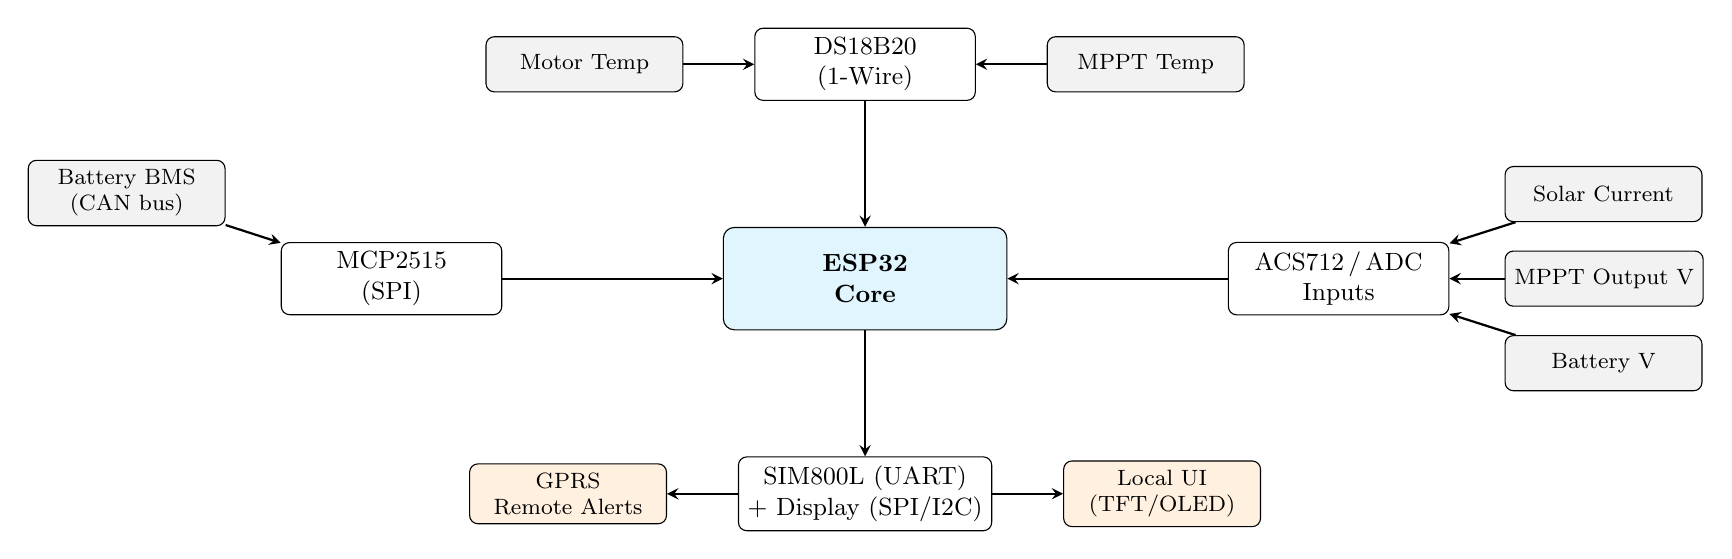
\begin{tikzpicture}[
    node distance=1.3cm and 1.8cm,
    box/.style={draw, rounded corners=3pt, fill=white, minimum width=2.8cm,
                minimum height=0.85cm, align=center, font=\small},
    core/.style={draw, rounded corners=4pt, fill=cyan!12, minimum width=3.6cm,
                 minimum height=1.3cm, align=center, font=\small\bfseries},
    sensor/.style={draw, rounded corners=3pt, fill=gray!10, minimum width=2.5cm,
                   minimum height=0.7cm, align=center, font=\footnotesize},
    outnode/.style={draw, rounded corners=3pt, fill=orange!12, minimum width=2.5cm,
                minimum height=0.7cm, align=center, font=\footnotesize},
    arr/.style={->, >=stealth, thick},
]
% ESP32 core
\node[core] (esp32) {ESP32\\Core};

% Left — CAN / BMS
\node[box,  left=2.8cm of esp32] (mcp)    {MCP2515\\(SPI)};
\node[sensor, above left=0.2cm and 0.7cm of mcp] (bms) {Battery BMS\\(CAN bus)};
\draw[arr] (bms)  -- (mcp);
\draw[arr] (mcp)  -- (esp32);

% Top — Temperature
\node[box,  above=1.6cm of esp32]          (ds18)   {DS18B20\\(1-Wire)};
\node[sensor, left=0.9cm  of ds18]         (motorT) {Motor Temp};
\node[sensor, right=0.9cm of ds18]         (mpptT)  {MPPT Temp};
\draw[arr] (motorT) -- (ds18);
\draw[arr] (mpptT)  -- (ds18);
\draw[arr] (ds18)   -- (esp32);

% Right — Current / Voltage
\node[box,  right=2.8cm of esp32]          (adc)    {ACS712\,/\,ADC\\Inputs};
\node[sensor, above right=0.25cm and 0.7cm of adc]  (solarI) {Solar Current};
\node[sensor, right=0.7cm of adc]          (mpptV)  {MPPT Output V};
\node[sensor, below right=0.25cm and 0.7cm of adc]  (batV)   {Battery V};
\draw[arr] (solarI) -- (adc);
\draw[arr] (mpptV)  -- (adc);
\draw[arr] (batV)   -- (adc);
\draw[arr] (adc)    -- (esp32);

% Bottom — Output
\node[box,     below=1.6cm of esp32]       (comm)   {SIM800L (UART)\\+ Display (SPI/I2C)};
\node[outnode, left=0.9cm  of comm]        (gsm)    {GPRS\\Remote Alerts};
\node[outnode, right=0.9cm of comm]        (ui)     {Local UI\\(TFT/OLED)};
\draw[arr] (esp32) -- (comm);
\draw[arr] (comm)  -- (gsm);
\draw[arr] (comm)  -- (ui);
\end{tikzpicture}%
}
\caption{BAKO Motors Monitoring System --- Reference Architecture}
\label{fig:ref-arch}
\end{figure}

\subsubsection*{Reference Designs Reviewed}

Three existing reference designs informed this architecture. The ESP32 CAN bus logger (open-source, GitHub) provided the MCP2515-to-ESP32 SPI wiring pattern and interrupt-driven frame reception approach. The MPPT solar charge controller monitoring projects (EPever RS485 loggers) informed the multi-voltage measurement strategy and calibration methodology. The SIM800L ESP32 integration guides (SIMCOM official and community) established the hardware flow control wiring and AT command firmware structure used for cellular communication.

\subsubsection*{Key Architecture Decisions}

All sensor reads are performed sequentially within a cooperative main loop at defined polling intervals --- CAN frames at 10~ms, temperature at 1~s, voltage/current at 500~ms --- feeding a shared data structure that the publish and alert logic reads from. This single-threaded design ensures no inter-task synchronization is needed. Alert thresholds (temperature, voltage out-of-range, overcurrent) are evaluated centrally after each polling cycle and trigger cellular SMS dispatch if breached.

\clearpage

\section{Systems Architecture}

\subsection{System Overview Diagram}

\begin{figure}[H]
    \centering
    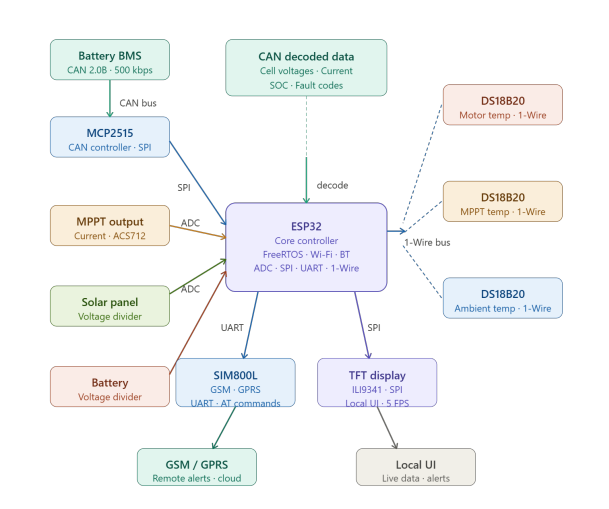
\includegraphics[width=0.85\textwidth]{images/arch-system-overview.png}
    \caption{ISS system architecture --- ESP32 core controller interfacing with the O'CELL BMS via MCP2515 CAN, three DS18B20 temperature sensors (1-Wire), ACS712 current sensors, voltage dividers, SIM800L GPRS cellular module, and local TFT display.}
    \label{fig:system-overview}
\end{figure}

The system is organised around a central ESP32 hub with five primary data flows: CAN bus communication with the BMS via MCP2515 SPI; DS18B20 digital temperature sensing on motor, MPPT, and DC/DC; ACS712/ACS758 analogue current measurement on solar panel and MPPT output; resistive divider voltage measurement at four nodes; and NPN handbrake detection. Data transmits over two parallel channels: a local Wi-Fi WebSocket server for dashboard access and a cellular GPRS/GPRS link to a cloud VPS via FastAPI into SQLite.

\subsection{Detailed System Block Diagram}

Figure~\ref{fig:diag-block} presents a detailed hardware and software block diagram of the full ISS system, from the vehicle sensors and BMS through the ISS PCB internals to the cloud backend and browser dashboard.

\begin{figure}[H]
    \centering
    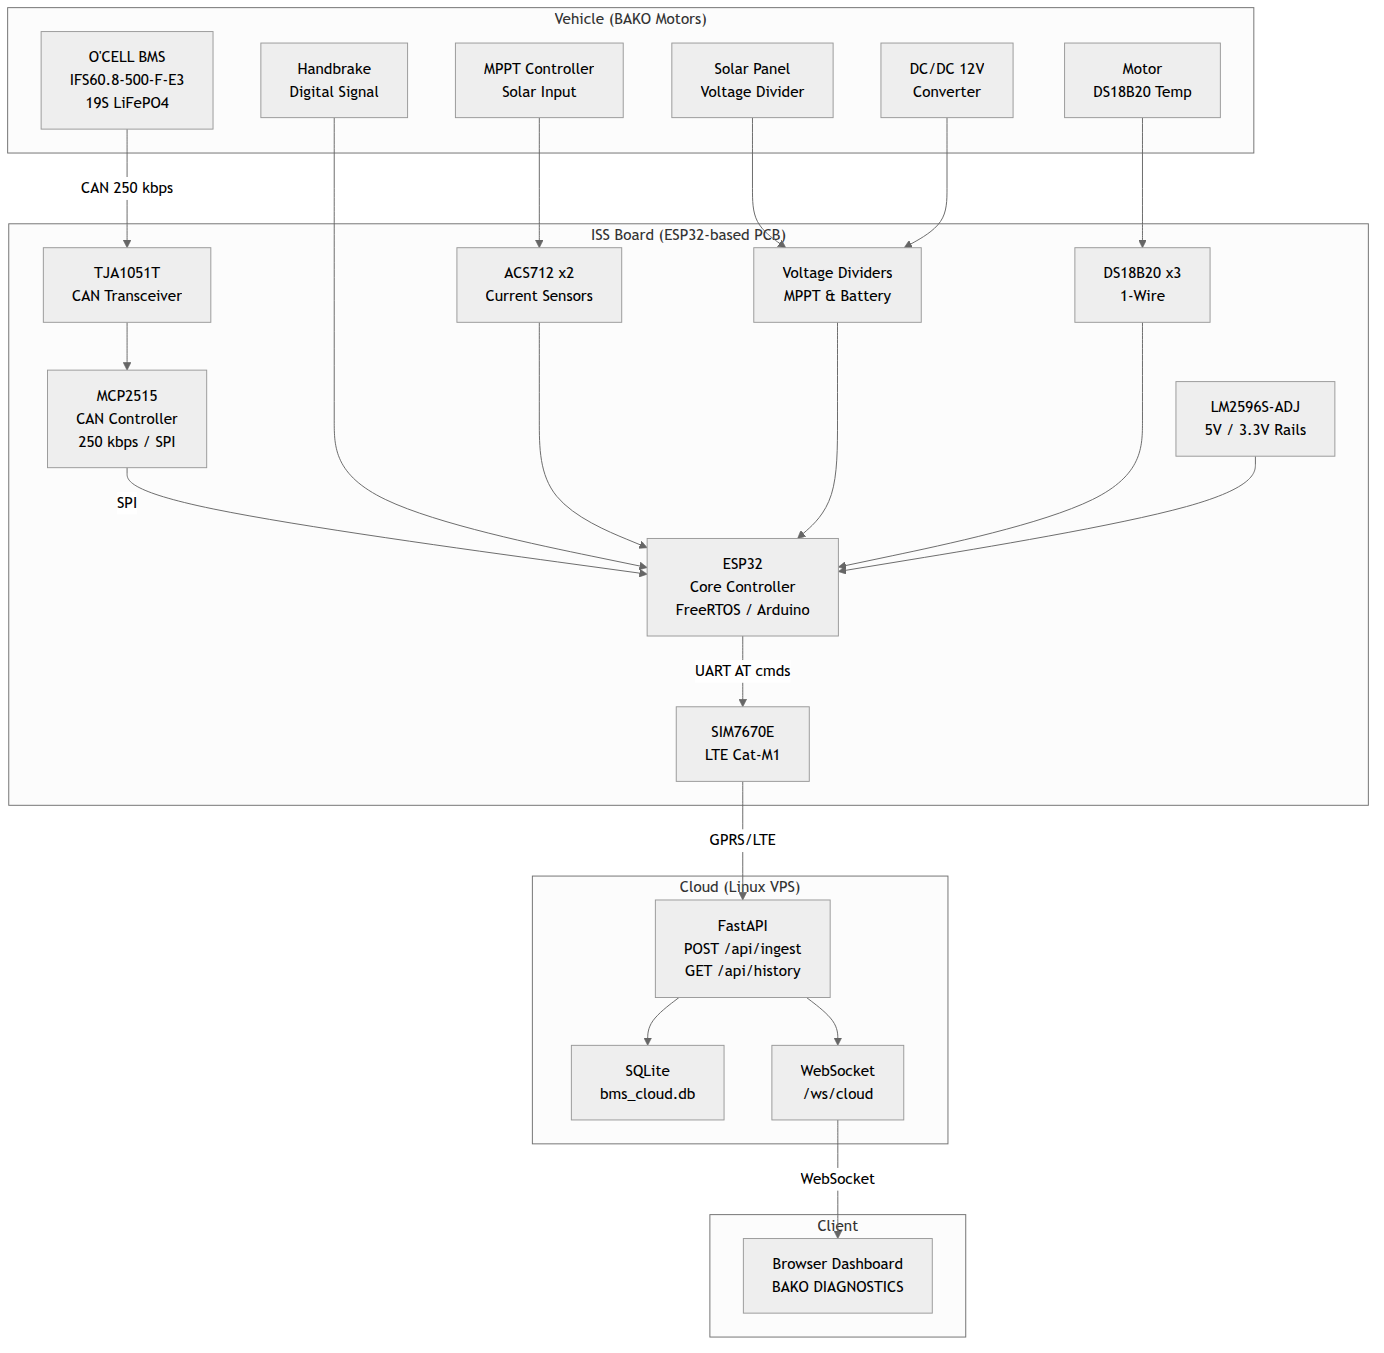
\includegraphics[width=\textwidth]{images/diag-block.png}
    \caption{Detailed ISS system block diagram showing all hardware subsystems (vehicle layer), ISS board internals (ESP32 peripherals and power regulation), cloud pipeline (FastAPI, SQLite, WebSocket), and browser client.}\label{fig:diag-block}
\end{figure}

\subsection{Electrical \& Power Systems}

The electrical and power subsystem is responsible for energy distribution, voltage regulation, and real-time monitoring of the vehicle's electrical parameters. The system integrates the battery pack, solar charging subsystem, MPPT controller, DC/DC converter, and embedded monitoring electronics.

The battery pack acts as the main energy source of the system~\cite{bakobattery} and is supervised by the Battery Management System (BMS)~\cite{ocellspec}. Communication with the BMS is established through the CAN Bus protocol~\cite{bakocan} using the MCP2515 CAN controller. The monitoring unit acquires important battery parameters such as pack voltage, current, state of charge, cell voltages, battery temperatures, and fault status information.

A solar energy subsystem is integrated to support power generation. The solar panel is connected to an MPPT (Maximum Power Point Tracking) controller, which optimises energy extraction efficiency. Current and voltage measurements are performed before and after the MPPT stage in order to evaluate charging performance and monitor power flow within the system.

The system also includes a DC/DC converter responsible for regulating voltage levels for low-power electronic components. Both input and output voltages of the converter are monitored to ensure stable operation and proper voltage regulation.

Electrical measurements are performed using ACS712 and ACS758 current sensors together with voltage sensing modules based on analogue voltage division. In addition, DS18B20 digital temperature sensors are installed on critical components such as the MPPT heatsink and DC/DC converter to supervise thermal behaviour and prevent overheating conditions.

The ESP32 microcontroller serves as the central processing and acquisition unit. It periodically collects sensor measurements and transmits the data through communication interfaces including CAN Bus, Wi-Fi, BLE, and GPRS/GPRS cellular connectivity.

\subsection{Electronic Control Units (ECUs)}

The monitoring platform integrates several Electronic Control Units (ECUs) responsible for data acquisition, communication, and system supervision. These units ensure reliable real-time monitoring of the vehicle's electrical and thermal parameters.

The main control unit of the system is the ESP32 microcontroller. It collects sensor measurements, decodes CAN Bus messages, processes data, and transmits information to the monitoring dashboard. Its integrated Wi-Fi and BLE capabilities make it suitable for embedded IoT applications.

The Battery Management System (BMS) supervises the battery pack by monitoring parameters such as voltage, current, temperature, state of charge (SOC), and fault conditions. Communication between the BMS and the ESP32 is achieved through the CAN Bus network using the MCP2515 CAN controller module.

Additional sensors are used to monitor the MPPT controller, DC/DC converter, solar panel, and motor temperature~\cite{bakomotor}. These measurements are periodically processed and transmitted by the ESP32.

During development, the ESP32 was also used as a firmware simulation platform to generate simulated sensor data and CAN frames. This allowed testing the dashboard and communication interfaces without continuously connecting the system to the vehicle, simplifying debugging and software validation.

Overall, the ECU architecture provides efficient monitoring, communication, and diagnostic capabilities for the vehicle monitoring platform.

\subsection{Embedded Software Architecture}
\label{sec:embedded-sw-arch}

The embedded software running on the ESP32 microcontroller is structured as a \textbf{single-threaded, cooperative loop} built on the Arduino framework. This architecture was chosen for its simplicity and determinism: all BMS-related tasks execute sequentially on one core, eliminating the need for inter-task synchronization.

The software is divided into five logical layers, shown in Figure~\ref{fig:sw-layers}:

\begin{figure}[H]
    \centering
    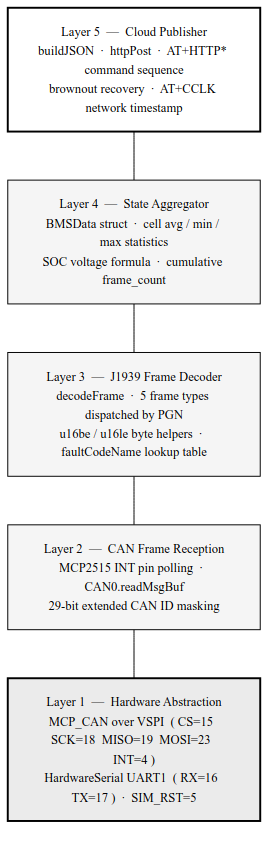
\includegraphics[width=0.45\textwidth]{images/sw-layers.png}
    \caption{ESP32 embedded software layer diagram}
    \label{fig:sw-layers}
\end{figure}

\begin{description}
    \item[Hardware Abstraction Layer (HAL)]
    Provides direct access to the MCP2515 via SPI (\texttt{mcp\_can} library) and to the SIM800L via HardwareSerial UART1. Pin assignments and bus parameters (CS, INT, baud rate, crystal frequency) are defined as constants and isolated from the application logic.

    \item[CAN Frame Reception]
    The MCP2515 asserts the \texttt{INT} line (GPIO 4) when a frame is placed in its receive buffer. The main loop polls this line and calls \texttt{CAN0.readMsgBuf()} to drain all pending frames. Extended CAN IDs are masked from the 29-bit field before processing.

    \item[J1939 Decoder]
    The \texttt{decodeFrame()} function dispatches each received frame by inspecting the \texttt{FUNC} byte of the CAN ID (bits 23--16). It handles five frame types (cell voltages, temperatures, BMS Basic 1 \& 2, charging request) and writes decoded values into the \texttt{BMSData} struct.

    \item[State Aggregator]
    The \texttt{BMSData} struct accumulates all decoded fields and maintains derived statistics (cell average, min, max, voltage-based SOC). The struct is updated in place and always holds the most recent complete state of the battery.

    \item[Cloud Publisher]
    Every 5 seconds, \texttt{buildJSON()} serializes \texttt{BMSData} into a JSON document using the ArduinoJson library, and \texttt{httpPost()} delivers it to the VPS via the SIM800L AT+HTTP* command set.
\end{description}

\subsubsection{Key Design Decisions}

\textbf{No explicit RTOS task management.} A FreeRTOS multi-task structure was considered but rejected because the single-responsibility loop handles all timing requirements naturally: CAN frames arrive at 100--500 ms intervals, and the publish cycle runs every 5 seconds. Adding preemptive scheduling would have introduced stack management and mutex overhead without any functional benefit.

\textbf{CAN drain during HTTP wait.} The \texttt{AT+HTTPACTION} response can take up to 30 seconds over a cellular link. To prevent the MCP2515 receive buffer (6 frames deep) from overflowing during this window, the HTTP wait loop polls the CAN \texttt{INT} pin and drains frames continuously, calling \texttt{decodeFrame()} in-place. This ensures the \texttt{BMSData} struct is fully up-to-date when the next publish cycle begins.

\textbf{HardwareSerial over SoftwareSerial.} SoftwareSerial operates via bit-banging and is sensitive to interrupt latency. The SIM800L produces multi-line AT response bursts that SoftwareSerial occasionally drops bytes from at 9600 baud on a loaded core. HardwareSerial UART1 uses dedicated silicon and a hardware FIFO, making it robust under all operating conditions.

% ─────────────────────────────────────────────────────────────────────────────
\subsection{Cloud \& Connectivity Architecture}
\label{sec:cloud-arch}

The cloud and connectivity architecture connects the on-vehicle ESP32 to a remote browser with minimal intermediaries. The full pipeline is shown in Figure~\ref{fig:cloud-arch}.

\begin{figure}[H]
    \centering
    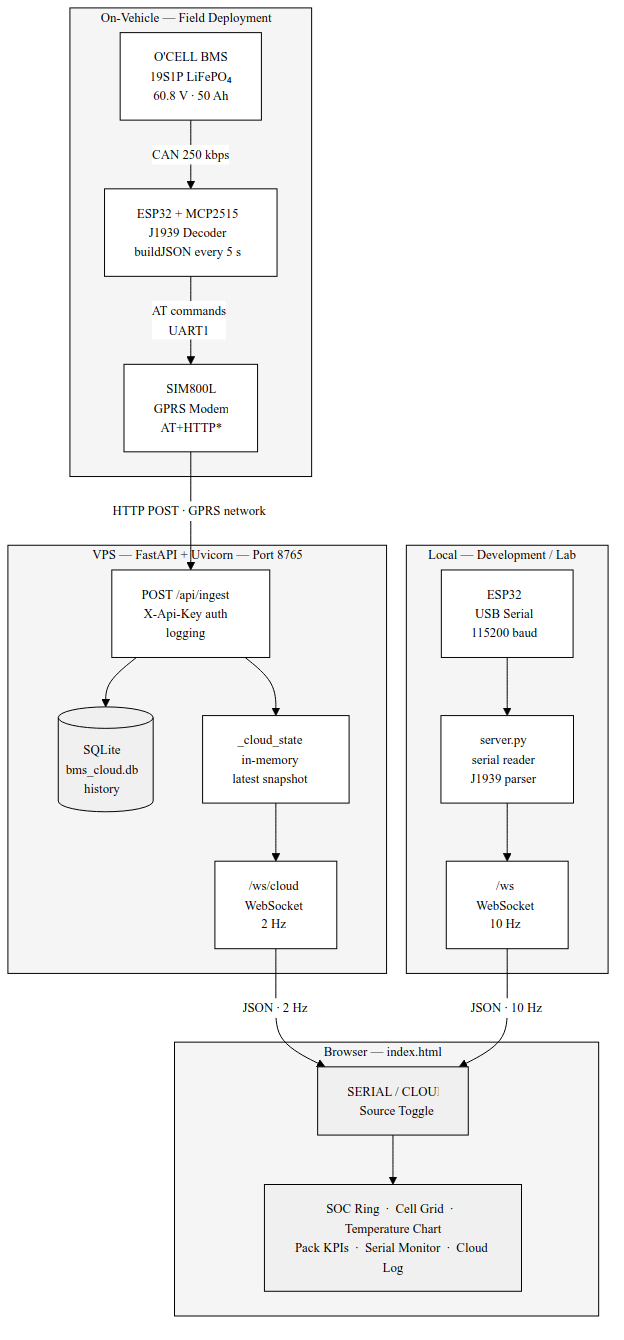
\includegraphics[width=0.5\textwidth]{images/cloud-arch.png}
    \caption{End-to-end cloud connectivity architecture}
    \label{fig:cloud-arch}
\end{figure}

\subsubsection{Component Roles}

\begin{description}
    \item[ESP32 + MCP2515 (On-vehicle edge node)]
    Reads and decodes SAE J1939 CAN frames from the BMS at up to 10 frames per second, aggregates them into a snapshot, and transmits one JSON document to the VPS every 5 seconds.

    \item[SIM800L GPRS Module]
    Provides wide-area cellular connectivity over GPRS Cat-M1 using the carrier network. Communicates with the ESP32 via AT commands over UART. Handles TCP/IP, HTTP, and DNS entirely on-chip using the AT+HTTP* service, so the ESP32 only needs to manage the AT command dialogue. The SIM800L-CORE footprint is used as the PCB layout placeholder; the physically populated component is the SIM800L.

    \item[VPS Backend (FastAPI + Uvicorn)]
    Acts as the single ingestion point and real-time relay for all cloud data. Receives POST requests from the ESP32, stores them to SQLite for persistence, and maintains an in-memory state that is pushed to connected browser clients via WebSocket at 2 Hz. The server also handles the SERIAL mode WebSocket, allowing the same dashboard to be used with a direct USB connection.

    \item[SQLite Database]
    Provides persistent local storage for all received snapshots. Enables historical data retrieval via the \texttt{/api/history} endpoint without any external database service.

    \item[Browser Dashboard]
    A single-page web application that renders live battery data received over WebSocket. Supports SERIAL mode (direct USB, 10 Hz) and CLOUD mode (VPS relay, 2 Hz). Auto-reconnects on network interruption.
\end{description}

\subsubsection{Data Flow Summary}

\begin{enumerate}
    \item O'CELL BMS $\rightarrow$ CAN bus (250 kbps, SAE J1939)
    \item ESP32 + MCP2515 $\rightarrow$ decode all frames $\rightarrow$ \texttt{BMSData} struct
    \item ESP32 $\rightarrow$ \texttt{buildJSON()} $\rightarrow$ JSON document
    \item ESP32 $\rightarrow$ SIM800L AT+HTTPACTION=1 $\rightarrow$ \texttt{POST /api/ingest} (HTTP, GPRS)
    \item VPS server $\rightarrow$ validate API key $\rightarrow$ SQLite insert + in-memory update
    \item VPS server $\rightarrow$ \texttt{/ws/cloud} WebSocket push every 2 s
    \item Browser $\rightarrow$ render panels (SOC, cells, temperatures, faults, cloud log)
\end{enumerate}

\subsubsection{Dual-Mode Operation}

A key architectural feature is that the dashboard supports two independent data sources via the same frontend interface. In \textbf{SERIAL mode}, the backend reads raw CAN log lines from the ESP32 USB serial port, decodes them through its own Python J1939 parser (\texttt{BMSState.decode()}), and pushes the result at 10 Hz. In \textbf{CLOUD mode}, the backend serves the latest snapshot received from the ESP32 over GPRS.

This dual-mode design provides two practical benefits:
\begin{itemize}
    \item During development and testing, the system can be operated entirely over USB without requiring a SIM card or GPRS connection.
    \item In the field, the dashboard can be opened from any web browser pointed at the VPS IP address, with no local software to install.
\end{itemize}

\subsection{3D Mechanical Architecture}

The 3D mechanical architecture of the ISS board is described in Chapter~7 (Mechanical Design). The two-layer PCB is dimensioned to fit within a standard DIN-rail enclosure, with all external connectors (CAN bus, sensor headers, power input) placed along the board perimeter for clean harness routing. A 3D render of the board is shown in Figure~\ref{fig:pcb-3d}.

\subsection{Safety \& Redundancy Design}

\subsubsection*{Hardware Protection}

Reverse polarity protection is implemented at the main power input using diode D6, which prevents damage to all downstream circuitry in the event of an incorrect supply connection. Overcurrent protection is provided by fuses F1, F2, and F3, placed on the main power rail and the sensor supply lines respectively, limiting fault currents before they can damage components. Zener diodes D3, D4, and D7 provide ESD and overvoltage clamping on the CAN bus lines, protecting the MCP2515 and TJA1051T transceiver from voltage spikes induced by the vehicle's electrical environment.

\subsubsection*{Software Redundancy}

A hardware watchdog timer ensures automatic recovery from firmware hangs by resetting the ESP32 microcontroller without requiring manual intervention. The MCP2515 CAN error counter is monitored continuously; if the error count exceeds the bus-off threshold --- which can occur after a transient disconnection or excessive noise on the CAN bus --- the driver automatically re-initialises the controller and resumes normal frame reception. All ADC input readings are subject to sanity-check bounds validation before being stored in the telemetry structure, discarding implausible values caused by transient noise or sensor disconnection. Threshold violation alerts for over-temperature, over-voltage, and over-current conditions are transmitted via SMS through the SIM800L module, enabling remote notification of critical fault events without requiring an active internet connection.

\clearpage

\section{Preparation Phase}

\subsection{Project Governance \& Team Structure}

The project is supervised academically by \textbf{Dr. Mortadha Dahmani} and conducted in direct collaboration with \textbf{BAKO Motors} as the industrial partner. The development team consists of seven members: Mahdi Hachicha, Mohamed Baccouche, Yassine Mtibaa, Hana Gdoura, Selima Grissa, Fares Smaoui, and Khadija Ben Hamida. Tasks are distributed across seven functional areas: hardware design and PCB, embedded firmware, GSM and cloud back-end, Wi-Fi and wireless dashboard, emulation and simulation, BLE wireless interface, and documentation and reporting. Version control is managed through Git with a shared private repository; task tracking and sprint planning follow a product backlog structure aligned with the Agile methodology described in Chapter~13.

\subsection{Development Environment Setup}

The embedded firmware is developed using \textbf{VS Code} with the \textbf{PlatformIO}~\cite{platformio} extension, targeting the ESP32 microcontroller with the Arduino-ESP32 framework. This toolchain provides dependency management, cross-compilation, and integrated serial monitoring in a single environment. PCB schematic capture and layout are performed in \textbf{KiCad 10.0}~\cite{kicad,snapeda,kicadforum}. The back-end server and Python sensor emulator are developed in \textbf{Python 3.11}. The cloud database runs on \textbf{SQLite} hosted on a Linux VPS, managed directly via the FastAPI server. All source code, PCB design files, and documentation are maintained in a private Git repository shared across the full team~\cite{github}. Component datasheets were retrieved from manufacturer websites and \texttt{alldatasheet.com}~\cite{alldatasheet}; tutorial resources were drawn from YouTube~\cite{youtube} and Google Scholar~\cite{googlescholar}. Technical writing assistance used Claude~AI~\cite{claudeai}.

\subsection{Simulation \& Prototyping Environment}

A Python-based sensor emulator was developed to simulate the complete vehicle sensor network, generating realistic values for 14 sensors with smooth, continuous transitions between states. The emulator cycles through seven test scenarios every 30 seconds:

\begin{itemize}
    \item \textbf{Normal Driving} --- typical operational parameters across all sensors.
    \item \textbf{Low Battery} --- state of charge below 20\%, reduced motor performance.
    \item \textbf{Charging Mode} --- MPPT active, battery current positive.
    \item \textbf{High Solar Input} --- peak solar irradiance, maximum MPPT throughput.
    \item \textbf{Night Mode} --- no solar input, battery discharging only.
    \item \textbf{Handbrake Fault} --- handbrake sensor engaged while vehicle is moving.
    \item \textbf{Overheat Condition} --- motor and DC/DC converter temperatures above threshold.
\end{itemize}

The emulator outputs structured JSON payloads compatible with the back-end API, fully replacing the physical ESP32 for end-to-end testing. In addition, a breadboard prototype was assembled early in the project to validate CAN bus wiring with the MCP2515, DS18B20 one-wire reading, and voltage divider scaling before committing to PCB layout.

\subsection{Risk Register (Initial)}

Initial risks identified at project outset included: the proprietary O'CELL BMS CAN protocol requiring reverse engineering before frame decoding could begin; ADC accuracy limitations on the ESP32 requiring dedicated calibration routines for precise voltage and current readings; component availability in Tunisia for specialised modules such as the SIM800L; GPRS network compatibility of the chosen cellular module with Tunisian operators (Ooredoo and Orange); and PCB fabrication lead times from local and regional manufacturers. Each risk was assigned a likelihood rating, an impact severity level, and a set of mitigation strategies as part of the project governance framework. The full expanded risk register is presented in Chapter~18.

\subsection{Procurement \& Vendor Selection}

All components were sourced through a two-channel strategy to balance cost, lead time, and availability. The ESP32-DEVKITC, MCP2515 SPI module, DS18B20 temperature sensors, ACS712 current sensors, passive components, and connectors were sourced locally in Tunisia from electronics distributors, keeping procurement costs low and eliminating import lead times. The SIM800L GSM/GPRS module was ordered through an online distributor with confirmed stock, given its unavailability in local markets. The PCB is specified for fabrication in FR-4, two copper layers, 1.6~mm board thickness, 35~\textmu m copper weight per layer, using standard KiCad Gerber RS-274X export for submission to the fabrication house.

\subsection{Prototype Planning}

The prototype was developed through five sequential phases, each building on validated hardware from the previous stage.

\textbf{Phase P1 --- Breadboard Proof of Concept (Weeks~3--6).}
Individual subsystems were validated in isolation on a breadboard. A single MCP2515 module was wired to an ESP32 via SPI to confirm CAN frame reception from the O'CELL BMS. One DS18B20 sensor was read over 1-Wire and its output printed to the serial monitor. An ACS712 current sensor output was sampled through the ESP32 ADC and calibrated against a bench power supply. Voltage divider networks were assembled and the scaling coefficients verified with a multimeter. Success criterion: all four subsystems operational and producing plausible readings independently.

\textbf{Phase P2 --- Integrated Breadboard (Weeks~7--9).}
All validated subsystems were connected to a single ESP32 simultaneously. A cooperative main loop was implemented to sequentially poll CAN, 1-Wire, and ADC inputs. The SIM800L GSM/GPRS module was connected via UART and an SMS alert was successfully dispatched. A local display (TFT LCD) was added to show live sensor data without a connected computer. Success criterion: all subsystems operational together without starvation over a 30-minute run.

\textbf{Phase P3 --- Semi-Permanent Stripboard Build (Week~10).}
The integrated breadboard design was transferred to stripboard for mechanical stability during field testing at the BAKO Motors workshop. Wiring was shortened and secured, and connectors were added for the CAN bus, temperature sensors, and power supply. This build was used for the first on-vehicle test with the actual O'CELL BMS CAN bus. Success criterion: reliable operation during vehicle movement with no loose connections or intermittent failures.

\textbf{Phase P4 --- Custom PCB Prototype (Weeks~10--13).}
Lessons learned from the stripboard build were incorporated into a KiCad schematic and PCB layout. The two-layer FR-4 board (Revision RECTIFICATION\_2) includes functional zoning for power, digital, CAN, and sensor domains, ESD protection Zener diodes on CAN lines, and fuse protection on all supply rails. Three MCP2515 SPI module headers support multi-bus configurations. The board was submitted for fabrication and populated by the team. Success criterion: board powers up correctly; all subsystems reachable from the ESP32 without errors.

\textbf{Phase P5 --- Integration Testing (Week~14).}
The fully populated PCB was connected to the vehicle harness and the cloud back-end. All sensor data paths were verified end-to-end: CAN frames decoded and displayed on the dashboard, temperature and current readings visible in the browser, and cloud telemetry appearing in the SQLite database on the VPS. The Python emulator was run in parallel to validate that the back-end API processed both hardware and emulated data identically.

\medskip
\begin{samepage}
\noindent\textbf{Quantitative success criteria applied across all phases:}
\begin{itemize}
    \item CAN frame reception rate $\geq 99\%$ over a 60-minute continuous test.
    \item DS18B20 temperature accuracy within $\pm 1$\textdegree{}C of a reference thermometer.
    \item ACS712 current measurement error $< 2\%$ of full scale.
    \item Voltage divider readings within $\pm 1\%$ of the multimeter reference.
    \item Cloud telemetry delivered to the VPS database with no snapshot loss over a 1-hour test.
\end{itemize}
\end{samepage}

\clearpage

\section{Circuit Design \& Electronics}

\subsection{Components Selection \& Justification}

Every electronic component for this project was chosen through a structured evaluation against four consistent criteria: technical fit with the system architecture, library and toolchain support, compatibility with Tunisian operator networks where applicable, and local availability in Tunisia together with unit cost.

\paragraph{Microcontroller --- ESP32-DEVKITC.}
The MCU is the brain of the ISS board. It must handle CAN data acquisition, sensor reading, GPRS connectivity, and real-time telemetry transmission simultaneously. The ESP32 integrates Wi-Fi, Bluetooth, and a dedicated UART for the GPRS module in a single chip, removing the need for extra communication modules~\cite{esp32datasheet}. Its compatibility with the Arduino IDE and the large IoT library ecosystem significantly accelerated development. The WROOM module is widely available locally in Tunisia and costs approximately 30~TND, making it the most practical and cost-effective choice.

\paragraph{CAN Controller --- MCP2515.}
The CAN controller acts as the interface between the ESP32 and the vehicle CAN bus. Three options were evaluated: the ESP32's built-in TWAI peripheral, the legacy SJA1000, and the MCP2515. Although the ESP32 includes a built-in CAN peripheral, it is only accessible through the ESP-IDF framework, making it significantly harder to integrate with Arduino-style libraries. The MCP2515 communicates over SPI, keeping wiring simple and reliable~\cite{mcp2515datasheet}. Its well-documented \texttt{mcp\_can} library and local availability in Tunisia made it the most practical choice. Three MCP2515 SPI module headers (J17, J18, J19) are present on the board to support multi-bus configurations.

\paragraph{CAN Transceiver --- TJA1051T.}
The CAN transceiver translates the digital logic signals from the MCP2515 into the differential voltage levels required on the physical CAN bus~\cite{iso11898}. The TJA1051T is an automotive-grade transceiver that operates at 5~V, directly matching the MCP2515 supply rail~\cite{tja1051datasheet}. It provides robust bus fault protection suited for the electrically noisy environment of a vehicle. It is the standard companion chip to the MCP2515 in OBD and automotive data-logging applications, ensuring long-term reliability.

\paragraph{Cellular Module.}
The SIM800L relies on 2G connectivity, which is being progressively phased out by Tunisian operators, making it a short-lived solution. The SIM800L supports 4G GPRS Cat-M1 and NB-IoT, is confirmed compatible with both Ooredoo and Orange networks in Tunisia, and remains future-proof as the country's network infrastructure continues to evolve. Its low operating cost further justified this selection. The KiCad schematic uses the SIM800L-CORE footprint as a physical layout placeholder; the component actually populated on the board is the SIM800L as noted in Section~\ref{sec:components-inventory}.

\paragraph{Power Regulation.}
The board is powered from the vehicle's 12~V rail. The LM2596S-ADJ is a switching buck regulator capable of delivering up to 3~A with approximately 90\% efficiency, producing minimal heat compared to a linear regulator~\cite{lm2596datasheet}. Its adjustable output (1.25~V to 37~V) allows the same component to supply both the 3.3~V ESP32 circuit and a 5~V rail. The board also carries an AMS1117 (V3.3) and an LM7805 (V5) for localised regulation where switching noise is undesirable.

\subsection{Circuit Schematic Description}

\begin{figure}[H]
    \centering
    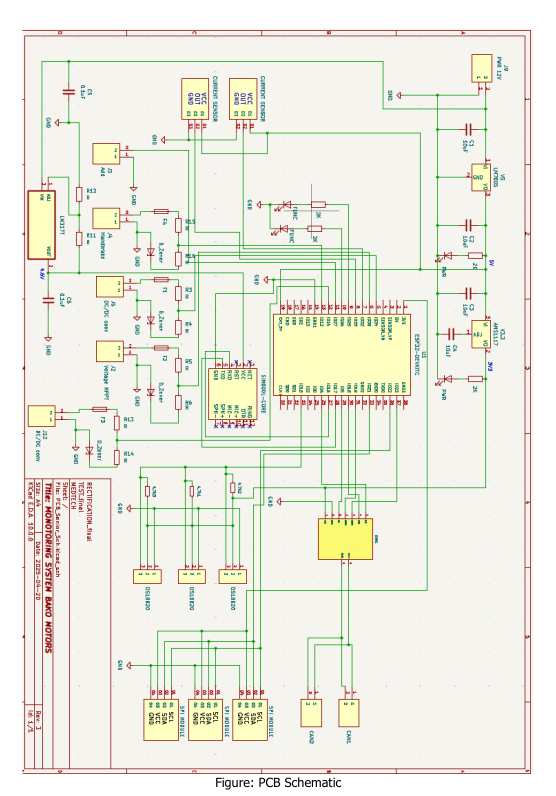
\includegraphics[width=\textwidth]{images/schematic-full.png}
    \caption{Complete ISS board circuit schematic (KiCad EEschema, Rev.~RECTIFICATION\_2).}
    \label{fig:schematic-full}
\end{figure}

The complete schematic is organised into five functional zones visible across the sheet: the ESP32-DEVKITC and SIM800L communication block in the upper centre, the MCP2515 CAN subsystem at the left, the DS18B20 1-Wire temperature sensor cluster at the lower left, the ACS712 analogue current sensor inputs at the lower right, and the power regulation and protection circuitry spanning the right edge. All inter-block signal paths are labelled with net names for traceability during PCB layout and debugging.

\begin{figure}[H]
    \centering
    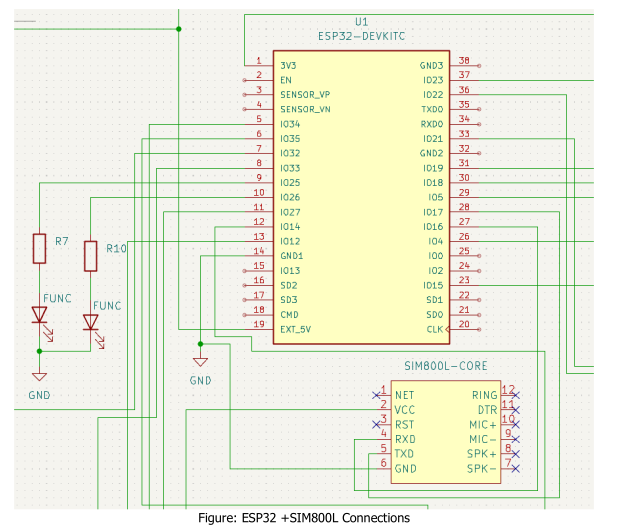
\includegraphics[width=0.85\textwidth]{images/schematic-esp32-sim.png}
    \caption{ESP32-DEVKITC and SIM800L cellular module connections: UART, level-shift resistors R7--R10, and status LEDs.}
    \label{fig:schematic-esp32-sim}
\end{figure}

The ESP32 UART1 (GPIO 16/17) connects to the SIM800L module through resistors R7--R10, which form a 2~k$\Omega$ voltage divider on each line to shift the 3.3~V ESP32 logic down to the 1.8~V interface level required by the SIM800L. LEDs D2 and D5, connected through current-limiting resistors, provide visual indication of firmware operating state: D2 pulses on each CAN frame received, and D5 lights during an active GPRS transmission.

\begin{figure}[H]
    \centering
    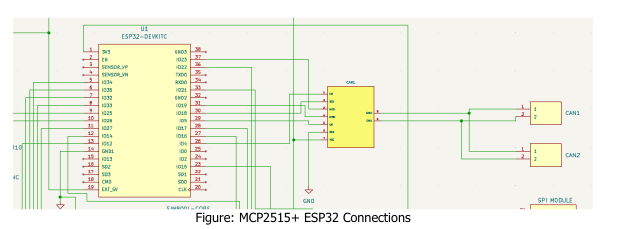
\includegraphics[width=\textwidth]{images/schematic-can.png}
    \caption{MCP2515 SPI CAN controller and TJA1051T transceiver connection detail including ESD Zener diodes D3, D4, D7.}
    \label{fig:schematic-can}
\end{figure}

The MCP2515 SPI module is connected to the ESP32 VSPI bus (SCK, MISO, MOSI) with a dedicated Chip Select line, allowing up to three independent CAN controllers to share the same SPI bus using separate CS signals. The TJA1051T transceiver converts the 3.3~V MCP2515 logic into the $\pm$2~V differential CAN\_H/CAN\_L bus signals required by the ISO~11898 physical layer standard. Zener diodes D3, D4, and D7 clamp any transient voltage spike on the CAN bus lines to safe levels before they reach the transceiver input pins.

\begin{figure}[H]
    \centering
    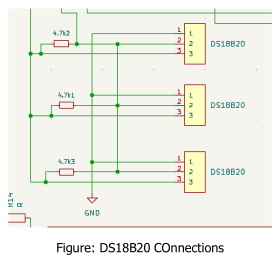
\includegraphics[width=0.55\textwidth]{images/schematic-ds18b20.png}
    \caption{Three DS18B20 temperature sensor connections (J6, J7, J8) with 4.7~k$\Omega$ 1-Wire pull-up resistors.}
    \label{fig:schematic-ds18b20}
\end{figure}

All three DS18B20 sensors share a single 1-Wire data line, which is pulled up to 3.3~V through one of the 4.7~k$\Omega$ resistors. Each sensor is factory-programmed with a unique 64-bit ROM address, allowing the ESP32 firmware to address them individually on the shared bus using the \texttt{DallasTemperature} library without any additional hardware. The three connectors (J6, J7, J8) are positioned at the board periphery so that the sensor cables can exit directly towards the motor, MPPT heatsink, and DC/DC converter mounting points.

\begin{figure}[H]
    \centering
    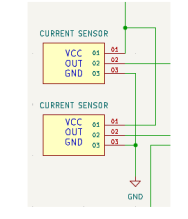
\includegraphics[width=0.45\textwidth]{images/schematic-sensors-current.png}
    \caption{Current sensor inputs: two ACS712 modules connected at J11 and J16 with analogue signal conditioning resistors.}
    \label{fig:schematic-sensors}
\end{figure}

Each ACS712 module produces an analogue output voltage centred at $V_{CC}/2$ (1.65~V) at zero current, shifting linearly at 66~mV/A for the 30~A variant used here. The signal conditioning resistors R3--R6 and R11--R14 provide a low-pass fiGPRSring and biasing network that suppresses high-frequency switching noise from the MPPT controller before the signal reaches the ESP32 ADC input, ensuring accurate current readings under electrically noisy vehicle conditions.

\begin{figure}[H]
    \centering
    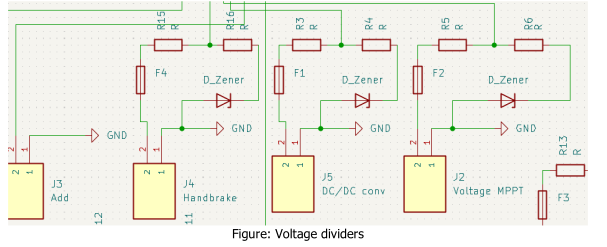
\includegraphics[width=\textwidth]{images/schematic-sensors-voltage.png}
    \caption{Voltage monitoring and auxiliary connectors: MPPT voltage divider (J2), DC/DC converter (J5), handbrake input (J4), auxiliary expansion (J3), with Zener clamp diodes D3, D4, D7 and signal conditioning resistors.}
    \label{fig:schematic-voltage-div}
\end{figure}

The MPPT output voltage, which can reach up to 50~V, is scaled down to the ESP32 ADC safe input range (0--3.3~V) using a resistive voltage divider. The Zener diodes D3, D4, and D7 clamp the ADC input line to prevent any overvoltage transient from damaging the ESP32's internal analogue circuitry. The handbrake connector J4 routes the digital handbrake signal through a pull-up resistor to a standard digital GPIO input, and the auxiliary connector J3 provides four uncommitted GPIO-connected pads for future sensor expansion.

The circuit schematic represents the logical connections between all electronic components before they are translated into physical copper traces on the PCB. The design is organised around five functional blocks.

The \textbf{ESP32-DEVKITC} (U1) is the central processing unit. It interfaces with the SIM800L cellular module (U2, using the SIM800L-CORE footprint) over UART for GPRS telemetry. The 2~k$\Omega$ resistors R7--R10 serve as UART voltage-level dividers between the 3.3~V ESP32 and the module's interface pins, protecting both ICs from logic-level mismatches. Functional status LEDs D2 and D5 indicate active operation states.

The \textbf{CAN subsystem} connects the MCP2515 SPI module to the ESP32 via SPI (Chip Select, MOSI, MISO, SCK lines), with individual chip-select pins allowing independent addressing of each CAN channel. The physical CAN layer is handled by the TJA1051T transceiver (CAN1 footprint), which interfaces with the primary CAN connector J1. A secondary CAN connector J10 provides a redundant bus connection. Zener diodes D3, D4, and D7 provide ESD and overvoltage clamping on the CAN bus lines. The 4.7~k$\Omega$ resistors (4.7k1, 4.7k2, 4.7k3) serve as bus pull-ups.

The \textbf{temperature sensing subsystem} accommodates three DS18B20 digital sensors connected via 1-Wire protocol through connectors J6, J7, and J8. The 4.7~k$\Omega$ resistors provide the mandatory pull-up on the 1-Wire data line.

The \textbf{analogue sensor subsystem} routes two current sensor inputs through J11 and J16, with signal conditioning resistors R3--R6 and R11--R14 adapting the sensor output levels to the ESP32 ADC input range. Voltage monitoring from the MPPT controller is received through J2. The handbrake digital signal is acquired through J4, providing vehicle state context for the supervision logic. Auxiliary expansion is available via connector J3.

The \textbf{protection layer} is integrated throughout the schematic. Reverse polarity protection is implemented at the main power input using diode D6. Overvoltage and ESD protection on the CAN bus is provided by Zener diodes D3, D4, and D7. Fuses F1, F2, and F3 provide overcurrent protection for the main power rail, sensor supplies, and auxiliary circuits respectively. The resistor network throughout the board ensures correct voltage levels at every inter-IC interface, preventing damage from logic-level mismatches.

\subsection{PCB Layout \& Design}

\begin{figure}[H]
    \centering
    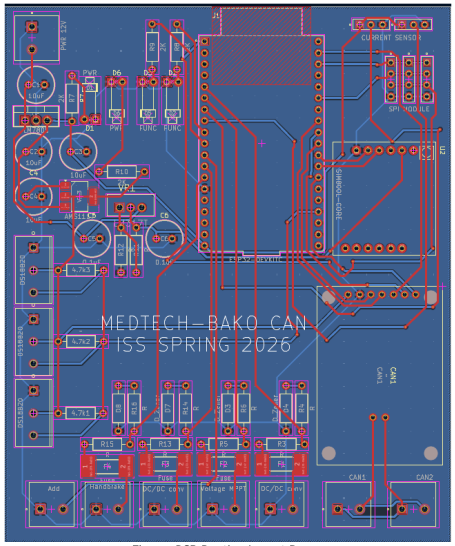
\includegraphics[width=0.75\textwidth]{images/pcb-routing.png}
    \caption{ISS board PCB routing layout (KiCad PCBnew, Rev.~RECTIFICATION\_2) showing F.Cu signal traces and B.Cu ground plane.}
    \label{fig:pcb-routing}
\end{figure}

The routing view shows all copper traces on the F.Cu (signal) layer in red and the B.Cu (ground plane) in blue. Short, direct routing of the SPI traces between the ESP32 and the MCP2515 modules minimises propagation delay and parasitic capacitance on the high-speed clock line (up to 10~MHz). Power traces carrying the 12~V input and 5~V CAN supply rails are given twice the width of signal traces to handle the required current without excessive resistive voltage drop.

\begin{figure}[H]
    \centering
    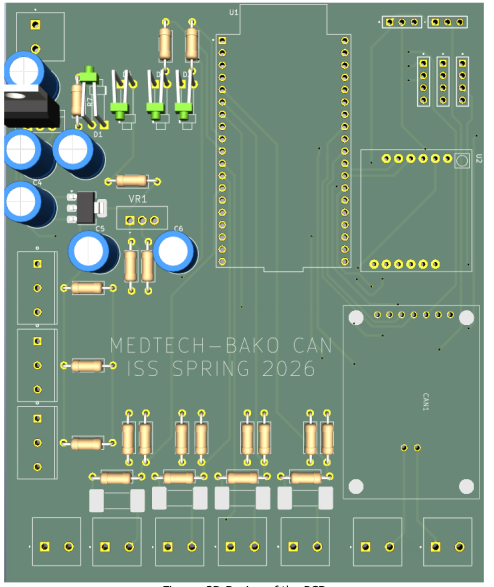
\includegraphics[width=0.75\textwidth]{images/pcb-3d.png}
    \caption{3D render of the ISS board (KiCad 3D viewer) showing component placement and board outline.}
    \label{fig:pcb-3d}
\end{figure}

The 3D render confirms correct physical clearances between tall components (electrolytic capacitors, SIM800L module, ESP32 devkit) and the board outline. The functional zoning is visible in the render: the power block occupies the top-right corner, the ESP32 and SIM800L module occupy the board centre, and the sensor connectors are distributed along the three remaining edges for clean harness routing. The board outline dimensions are compatible with a standard 100~mm $\times$ 100~mm DIN-rail enclosure footprint.

The PCB was designed using KiCad 10.0 PCBnew. Table~\ref{tab:pcb-params} summarises the key mechanical and electrical parameters of the board as extracted from the KiCad project file.

\begin{table}[H]
\centering
\caption{PCB Mechanical and Electrical Parameters}
\label{tab:pcb-params}
\begin{tabular}{>{\bfseries}p{4.2cm} p{8.0cm}}
\toprule
Parameter & Value \\
\midrule
Board title      & MONITORING SYSTEM BAKO MOTORS \\
Design revision  & RECTIFICATION\_2 (06 April 2026) \\
Layer count      & 2 layers (F.Cu + B.Cu) \\
Board thickness  & 1.6~mm \\
Copper thickness & 35~\textmu m (1~oz) per layer \\
Substrate material & FR-4 ($\varepsilon_r = 4.5$, loss tangent = 0.02) \\
Solder mask      & Both sides (front + back), 10~\textmu m \\
Silkscreen       & Front + Back \\
Min. track/spacing & Per KiCad DRC defaults \\
Via tenting      & Both sides \\
Design tool      & KiCad 10.0 / PCBnew \\
\bottomrule
\end{tabular}
\end{table}

With the two-layer stackup, the front copper layer (F.Cu) carries the majority of signal traces and component connections. The back copper layer (B.Cu) is used for the ground plane pour and power return paths, reducing electromagnetic interference and providing a low-impedance ground reference for all circuits. Critical high-frequency SPI traces connecting the ESP32 to the MCP2515 modules are kept short and routed on F.Cu to minimise parasitic inductance. Power traces carrying the 12~V input, 5~V CAN rail, and 3.3~V logic rail are given increased width to handle the required current without excessive resistive heating. Sensor signal traces, particularly the 1-Wire bus and analogue current-sense lines, are routed away from the switching regulator to avoid noise coupling.

The component placement follows a functional zoning approach to minimise cross-interference between the power, digital, and analogue sections of the board:

\begin{itemize}
    \item \textbf{Power zone:} The main power input connector (J9), fuses (F1--F3), LM2596S-ADJ (VR1), LM7805 (V5), and AMS1117 (V3.3) are grouped together to contain high-current paths and facilitate efficient heat dissipation.
    \item \textbf{Digital processing zone:} The ESP32-DEVKITC (U1) and SIM800L cellular module (U2) are placed centrally, minimising trace lengths to the SPI, UART, and GPIO peripherals.
    \item \textbf{CAN bus zone:} The MCP2515 SPI modules (J17--J19), TJA1051T transceiver, and CAN connectors (J1, J10) are grouped together at one edge of the board, simplifying external wiring harness routing to the vehicle OBD port~\cite{bakowiring}.
    \item \textbf{Sensor zone:} The DS18B20 connectors (J6--J8), current sensor inputs (J11, J16), and MPPT voltage input (J2) are placed at the board periphery, allowing sensor cables to exit cleanly without routing over the digital core.
\end{itemize}

The design was verified using KiCad's Design Rule Check (DRC) prior to export. Pad-to-mask clearance is set to 0~mm (controlled by the manufacturer's solder mask process). Via tenting is applied on both the front and back layers to prevent solder bridges and improve board reliability. The silk screen layers carry component reference designators and polarity markers to facilitate assembly and inspection. The board is ready for submission to a PCB fabrication house using standard Gerber RS-274X export from KiCad.

\subsection{Full Components Inventory}
\label{sec:components-inventory}

Tables~\ref{tab:bom-ics} and~\ref{tab:bom-passives} list all components populated on the ISS board as extracted from the KiCad PCB file (test2.kicad\_pcb, Rev.~RECTIFICATION\_2). References, values, quantities, and functional roles are provided for each entry.

\begin{table}[H]
\centering
\caption{Full Component Inventory --- Integrated Circuits and Connectors}
\label{tab:bom-ics}
\small
\begin{tabular}{>{\bfseries}p{2.4cm} p{3.2cm} c p{5.8cm}}
\toprule
Ref. & Component / Value & Qty & Function \\
\midrule
U1           & ESP32-DEVKITC        & 1 & Main MCU --- Wi-Fi, BT, UART to SIM800L \\
U2           & SIM800L-CORE*        & 1 & GPRS cellular module (SIM800L footprint) \\
V3.3         & AMS1117 (3.3\,V)     & 1 & 3.3\,V LDO for ESP32 I/O \\
V5           & LM7805               & 1 & 5\,V linear reg. for CAN side \\
VR1          & LM317T               & 1 & Adjustable voltage ref. / LM2596S-ADJ compatible \\
J1           & CAN1 connector       & 1 & Primary CAN bus interface \\
J10          & CAN2 connector       & 1 & Secondary / redundant CAN bus \\
J19/J17/J18  & SPI MODULE           & 3 & MCP2515 CAN controller via SPI \\
J11/J16      & CURRENT SENSOR       & 2 & Analogue current-sense inputs \\
J6/J7/J8     & DS18B20              & 3 & 1-Wire temperature sensors \\
J2           & Voltage MPPT         & 1 & MPPT voltage monitoring input \\
J4           & Handbrake            & 1 & Handbrake digital signal input \\
J5/J12       & DC/DC conv.          & 2 & Power conversion headers (LM2596S-ADJ) \\
J9           & PWR 12V              & 1 & 12\,V main power input connector \\
J3           & Add                  & 1 & Auxiliary / expansion connector \\
CAN1         & CAN transceiver      & 1 & TJA1051T CAN bus transceiver \\
F1/F2/F3     & Fuse                 & 3 & Overcurrent protection \\
D1           & PWR LED              & 1 & Power-on indicator \\
D2/D5        & FUNC LED             & 2 & Status / function indicators \\
D3/D4/D7     & D\_Zener             & 3 & Zener clamp / ESD protection \\
D6           & PWR diode            & 1 & Reverse-polarity / flyback protection \\
\bottomrule
\end{tabular}
\end{table}

\begin{table}[H]
\centering
\caption{Full Component Inventory --- Passive Components}
\label{tab:bom-passives}
\small
\begin{tabular}{>{\bfseries}p{2.4cm} p{3.2cm} c p{5.8cm}}
\toprule
Ref. & Component / Value & Qty & Function \\
\midrule
C1/C2/C3/C4 & 10~\textmu F cap       & 4 & Bulk decoupling capacitors \\
C5/C6        & 0.1~\textmu F cap      & 2 & High-freq. bypass capacitors \\
R7/R8/R9/R10 & 2~k$\Omega$ resistor & 4 & UART voltage-level dividers \\
4.7k1/2/3    & 4.7~k$\Omega$        & 3 & 1-Wire pull-up resistors (DS18B20) \\
R3/R5/R6, R11--R14 & Resistor (misc) & 7 & Signal conditioning \& biasing \\
R4           & 2~k$\Omega$          & 1 & UART/SIM interface level divider \\
\bottomrule
\end{tabular}
\end{table}

\noindent\small{* The SIM800L-CORE footprint reference in KiCad is used as the physical placeholder for the SIM800L module during layout. The component actually populated on the board is the SIM800L as justified in Section~6.1.}

\subsection{Component Photographs}
\label{sec:component-photos}

The photographs below show the physical components used to populate the ISS board prototype. Each image is accompanied by the reference designator and the role it fulfils in the circuit.

\begin{figure}[H]
\centering
\begin{minipage}[t]{0.30\textwidth}
    \centering
    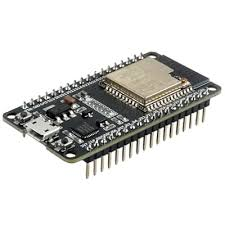
\includegraphics[width=\linewidth]{images/esp32.jpeg}
    \caption{ESP32-DEVKITC~V1 microcontroller. Central processing unit for CAN decoding, sensor acquisition, and GPRS telemetry.}
    \label{fig:photo-esp32}
\end{minipage}\hfill
\begin{minipage}[t]{0.30\textwidth}
    \centering
    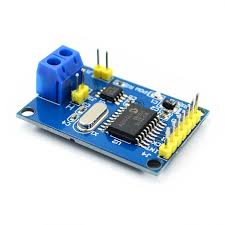
\includegraphics[width=\linewidth]{images/mcp2515.jpeg}
    \caption{MCP2515 SPI CAN controller module. Interfaces the ESP32 to the J1939 CAN bus via SPI (J17/J18/J19).}
    \label{fig:photo-mcp2515}
\end{minipage}\hfill
\begin{minipage}[t]{0.30\textwidth}
    \centering
    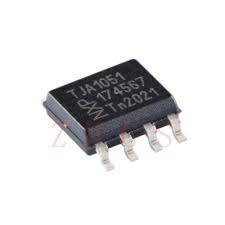
\includegraphics[width=\linewidth]{images/tja1051t.jpeg}
    \caption{TJA1051T automotive CAN transceiver. Converts MCP2515 logic levels to differential CANH/CANL bus signals.}
    \label{fig:photo-tja1051}
\end{minipage}
\end{figure}

\begin{figure}[H]
\centering
\begin{minipage}[t]{0.30\textwidth}
    \centering
    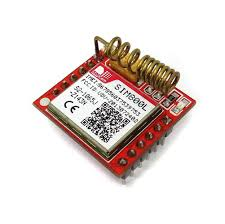
\includegraphics[width=\linewidth]{images/sim800l.jpeg}
    \caption{SIM800L GPRS Cat-M1 module. Provides 4G cellular connectivity to the VPS cloud backend via GPRS/GPRS.}
    \label{fig:photo-SIM800L}
\end{minipage}\hfill
\begin{minipage}[t]{0.30\textwidth}
    \centering
    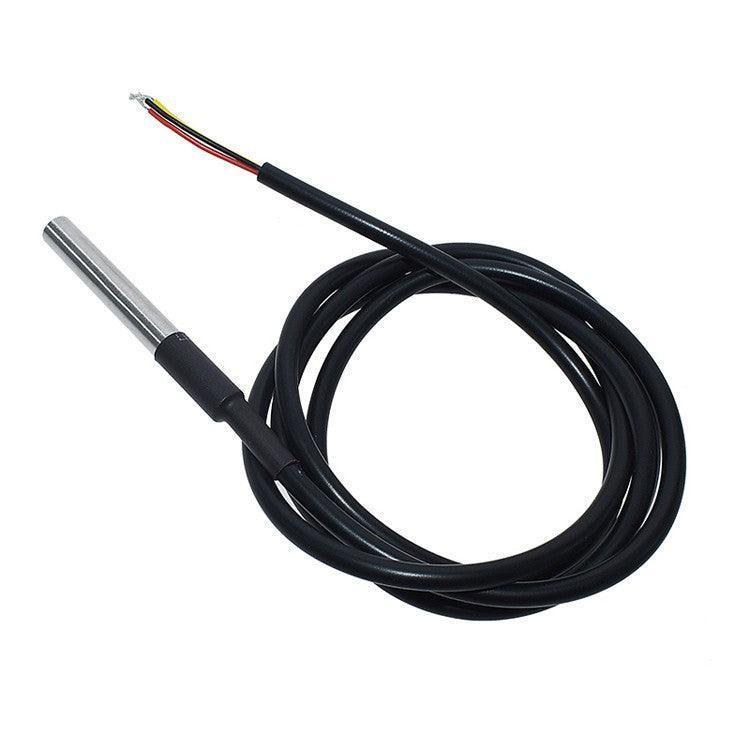
\includegraphics[width=\linewidth]{images/ds18b20-sonde-de-temperature-inoxydable-tuni-smart-innovation.jpg}
    \caption{DS18B20 1-Wire digital temperature sensors (J6, J7, J8). Monitor motor winding, MPPT heatsink, and DC/DC temperatures.}
    \label{fig:photo-ds18b20}
\end{minipage}\hfill
\begin{minipage}[t]{0.30\textwidth}
    \centering
    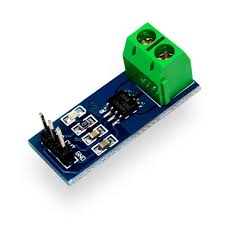
\includegraphics[width=\linewidth]{images/ACS712-30A.jpeg}
    \caption{ACS712-30A Hall-effect current sensor modules (J11, J16). Measure solar panel and MPPT output currents.}
    \label{fig:photo-acs712}
\end{minipage}
\end{figure}

\subsection{Design Summary}

The electronic design of the BAKO Motors ISS board is built around a carefully selected set of components that maximise functionality while remaining practical and cost-effective in the Tunisian market context. The ESP32 provides a powerful, affordable, and well-supported processing core. The MCP2515 and TJA1051T together form a robust, proven CAN bus interface fully compatible with the J1939 protocol used by the O'CELL BMS. The SIM800L ensures long-term GPRS network compatibility with local Tunisian operators, making it a future-proof choice over the 2G-only SIM800L. The LM2596S-ADJ provides efficient switching power conversion for the full board from the vehicle's 12~V rail.

The two-layer KiCad PCB design translates these component choices into a compact, well-organised board with clear functional zoning, adequate protection circuitry, and a layout strategy designed to minimise signal interference between the power, digital, and analogue domains. The design is at revision RECTIFICATION\_2, reflecting iterative refinement based on functional testing and layout optimisation. The board is ready for Gerber export and submission to a PCB fabrication house.

\clearpage

\section{3D Design \& Mechanical Engineering}

\subsection{Enclosure Design Overview}

The BAKO Motors ISS board requires a protective enclosure that shields the PCB from mechanical vibration, dust, and incidental contact with vehicle components, while still providing clear access to all external connectors and sensor cables. The enclosure was designed from scratch as a 3D-printable ABS/PLA part using parametric CAD software, sized to match the ISS board footprint and the connector layout established in the KiCad PCB (Rev.~RECTIFICATION\_2).

The design objectives were:
\begin{itemize}
    \item \textbf{Secure board mounting} — four corner bosses with through-holes accept M3 screws that fasten the PCB directly to the enclosure floor without additional standoffs.
    \item \textbf{Cable egress slots} — rectangular cutouts on two opposing side walls accommodate the vehicle harness connectors (CAN bus J1, power J9, sensor bundles) and the USB programming port without stressing the PCB edge connectors.
    \item \textbf{Open-top access} — the enclosure is a lidded tray; the open-top design allows heat generated by the LM2596S-ADJ switching regulator to dissipate naturally and provides easy PCB removal for re-flashing.
    \item \textbf{Brand identification} --- \textit{SMU-BAKO} and \textit{Senior CSE 2026} text is embossed on the exterior walls to identify the unit during installation.
\end{itemize}

\subsection{CAD Model}

The enclosure geometry was modelled in a parametric CAD environment. The model consists of a single-body rectangular tray with a uniform 2~mm wall thickness, an internal floor that matches the PCB outline, four corner mounting bosses, and two sets of rectangular cutouts on opposing side walls for the wiring harness.

Figures~\ref{fig:case-cad-front} and~\ref{fig:case-cad-side} show the CAD model from two isometric viewpoints, illustrating the cable egress slots and the embossed labelling on the exterior faces.

\begin{figure}[H]
    \centering
    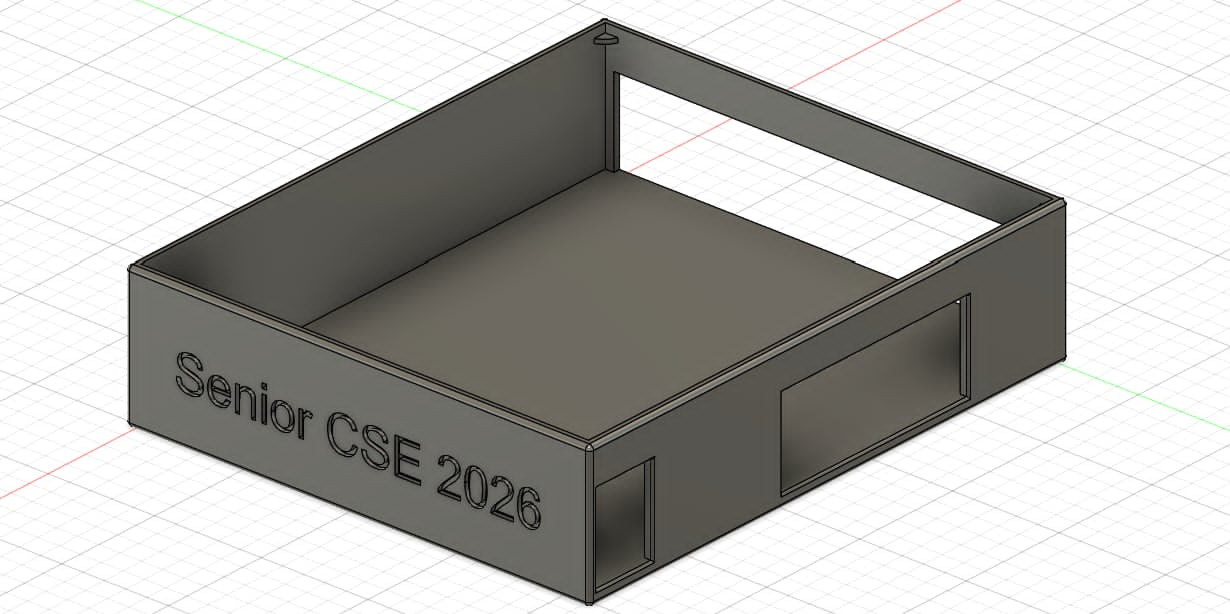
\includegraphics[width=0.82\textwidth]{images/Untitled.jpeg}
    \caption{ISS enclosure CAD model --- isometric front-right view showing the ``Senior CSE 2026'' embossed face and the rectangular connector cutout on the right side wall.}\label{fig:case-cad-front}
\end{figure}

\begin{figure}[H]
    \centering
    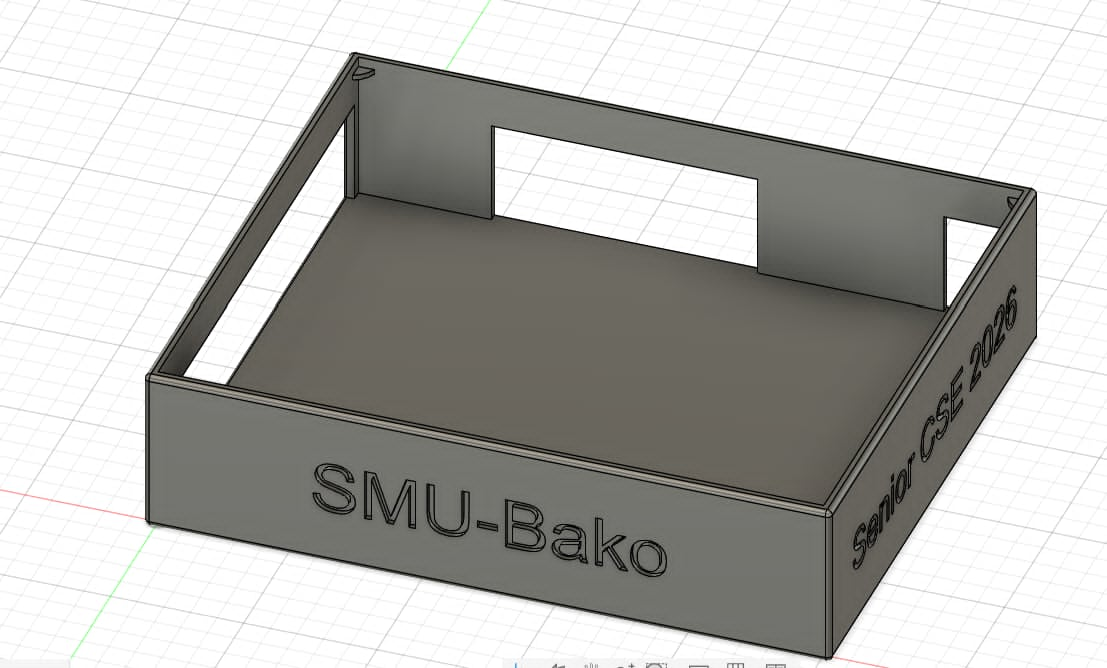
\includegraphics[width=0.82\textwidth]{images/Untitled1.jpeg}
    \caption{ISS enclosure CAD model --- isometric front-left view showing the ``SMU-Bako'' and ``Senior CSE 2026'' embossed faces and the cable egress slots on two walls.}\label{fig:case-cad-side}
\end{figure}

\subsection{3D Print Preparation \& Slicing}

The CAD model was exported as an STL file and imported into \textbf{Bambu Studio} for print preparation. Bambu Studio's slicer was used to orient the part, generate support structures, and configure print parameters for a Bambu Lab printer with a textured PEI plate. The enclosure prints in a single session without post-processing assembly.

Figures~\ref{fig:case-slicer-a},~\ref{fig:case-slicer-b}, and~\ref{fig:case-slicer-c} show the sliced model from three orientations in the Bambu Studio build plate preview, confirming correct orientation (open face up), corner mounting feet visible from all angles, and no unsupported overhangs requiring internal supports.

\begin{figure}[H]
    \centering
    \begin{subfigure}[b]{0.48\textwidth}
        \centering
        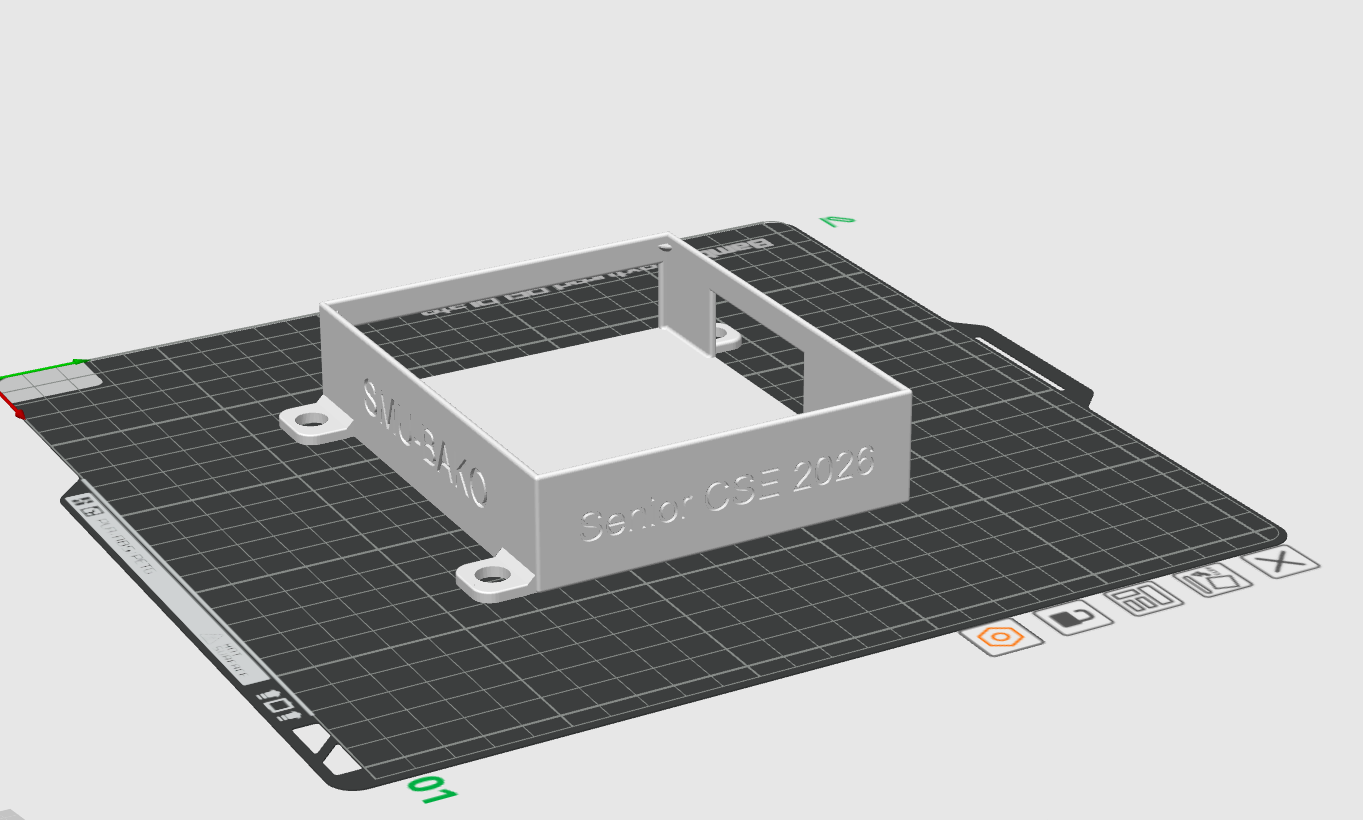
\includegraphics[width=\textwidth]{images/1.PNG}
        \caption{Isometric front-right --- ``SMU-BAKO / Senior CSE 2026'' labelling and mounting corner feet visible.}\label{fig:case-slicer-a}
    \end{subfigure}
    \hfill
    \begin{subfigure}[b]{0.48\textwidth}
        \centering
        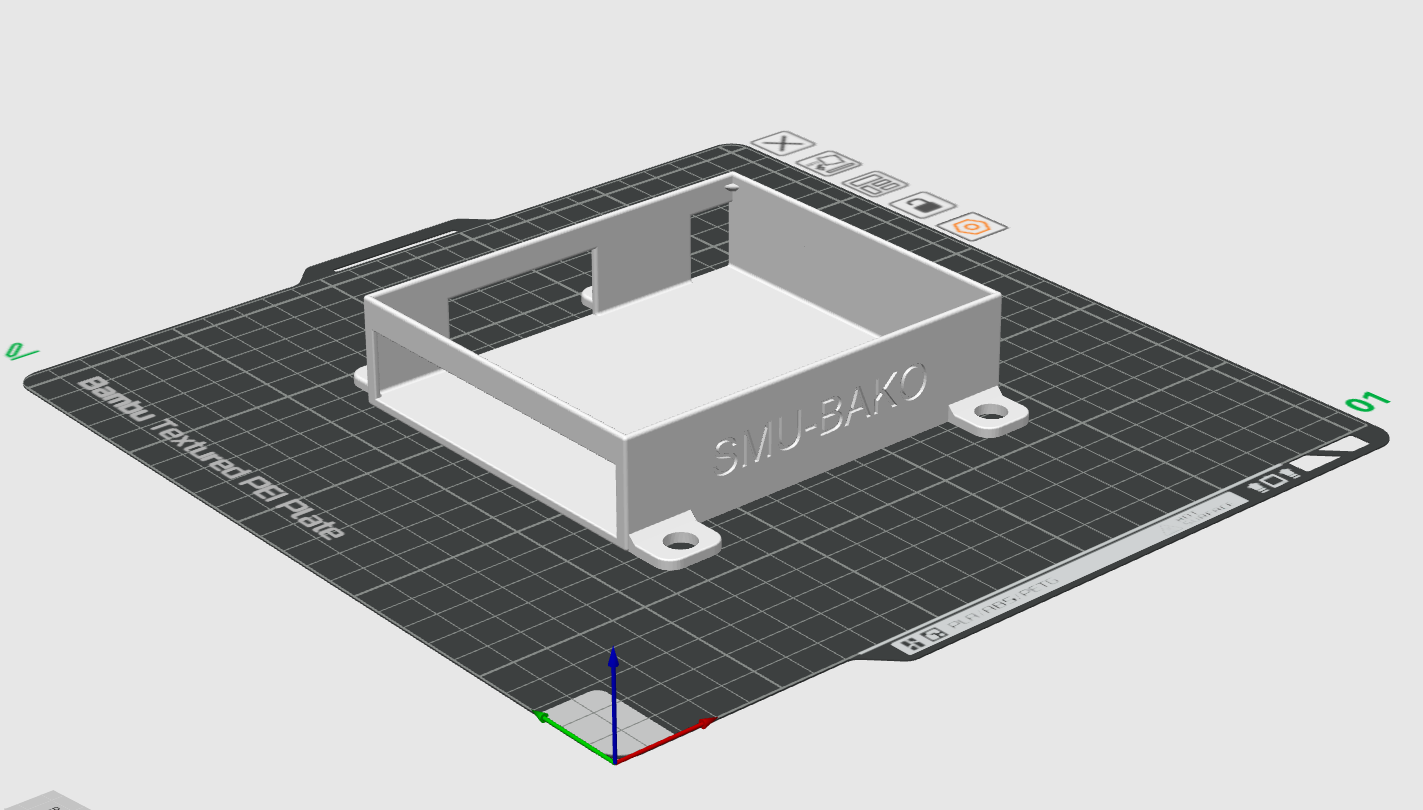
\includegraphics[width=\textwidth]{images/2.PNG}
        \caption{Isometric front-left --- front cable egress slot and open-top orientation confirmed.}\label{fig:case-slicer-b}
    \end{subfigure}

    \vspace{0.5em}

    \begin{subfigure}[b]{0.65\textwidth}
        \centering
        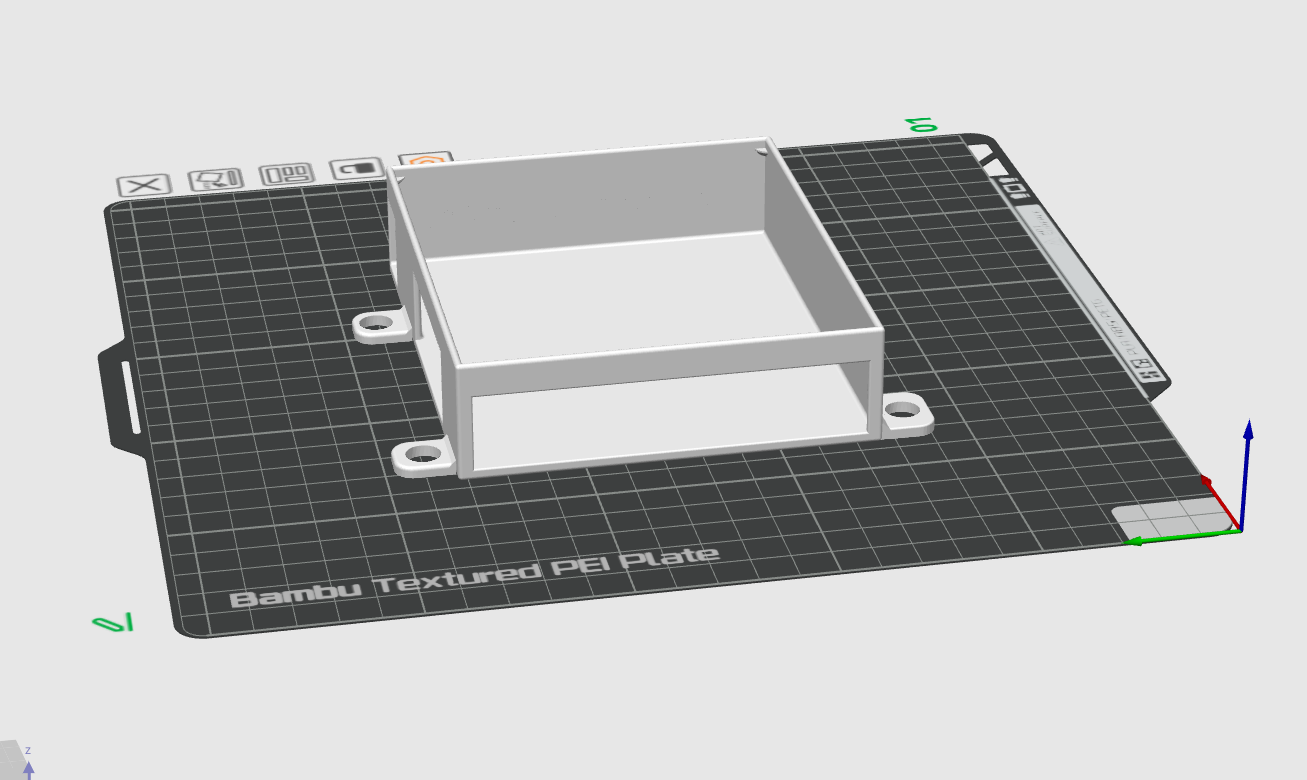
\includegraphics[width=\textwidth]{images/3.PNG}
        \caption{Rear isometric view --- two back-wall cutouts for the vehicle harness and CAN bus connector visible.}\label{fig:case-slicer-c}
    \end{subfigure}
    \caption{Bambu Studio slicer views of the ISS enclosure on the textured PEI build plate, shown from three orientations. The enclosure prints open-face-up with no supports required.}\label{fig:case-slicer-all}
\end{figure}

\subsection{Mechanical Features Summary}

Table~\ref{tab:case-features} summarises the key mechanical parameters of the enclosure as designed.

\begin{table}[H]
\centering
\caption{ISS Enclosure Mechanical Parameters}\label{tab:case-features}
\begin{tabular}{>{\bfseries}p{4.2cm} p{8.5cm}}
\toprule
Parameter & Value \\
\midrule
Design tool        & Parametric CAD (Fusion 360 / equivalent) \\
Slicer             & Bambu Studio \\
Print orientation  & Open face up, flat on build plate \\
Wall thickness     & 2~mm uniform \\
Material           & PLA or PETG (prototype); ABS for vehicle environment \\
Corner mounting    & 4$\times$ M3 boss, 6~mm diameter, through-hole for PCB screws \\
Cable egress slots & 2 side walls; rectangular cutouts sized for JST + screw-terminal connectors \\
Exterior labelling & ``SMU-BAKO'' and ``Senior CSE 2026'' embossed text, 0.5~mm depth \\
Protection rating  & Open-top prototype; IP-rated lid deferred to next revision \\
\bottomrule
\end{tabular}
\end{table}

The enclosure design is production-ready for the prototype phase. A sealed lid with gasket groove and SIM800L antenna pass-through is identified as a short-term development item for field deployment, targeting IP54 ingress protection as noted in the recommendations chapter (Section~\ref{sec:recommendations}).

\clearpage

\section{Software \& Code Implementation}

This section describes the software developed for the Bako OBD ISS platform, covering the embedded firmware running on the ESP32 microcontroller, the battery management decoding logic, the cloud publishing pipeline, and the validation strategy used to verify correct behavior at each layer.

% ─────────────────────────────────────────────────────────────────────────────
\subsection{Firmware Architecture \& RTOS Integration}

The ESP32 firmware is built on the \textbf{Arduino framework} using the \textbf{PlatformIO} build system~\cite{platformio}, which provides dependency management, cross-compilation, and serial monitoring in a single toolchain. Although the Arduino framework does not expose the underlying FreeRTOS scheduler directly, the ESP32's dual-core architecture is leveraged implicitly: the Arduino \texttt{loop()} function executes on Core 1 while the Wi-Fi/Bluetooth stack occupies Core 0. All BMS-related tasks — CAN frame reception, state accumulation, and HTTP publishing — run sequentially on Core 1 without preemption, which simplifies state management and eliminates the need for mutexes at the firmware level.

The firmware follows a \textbf{cooperative, interrupt-driven} model. The MCP2515 CAN transceiver asserts an active-low \texttt{INT} line (GPIO 4) each time a new frame is placed in its receive buffer. The main loop polls this pin continuously and drains all pending frames before entering the timed publish cycle. This design ensures that no CAN frame is ever dropped due to buffer overflow, even during the longer HTTP transaction window.

The overall execution model is summarized in Figure~\ref{fig:fw-flow}.

\begin{figure}[H]
    \centering
    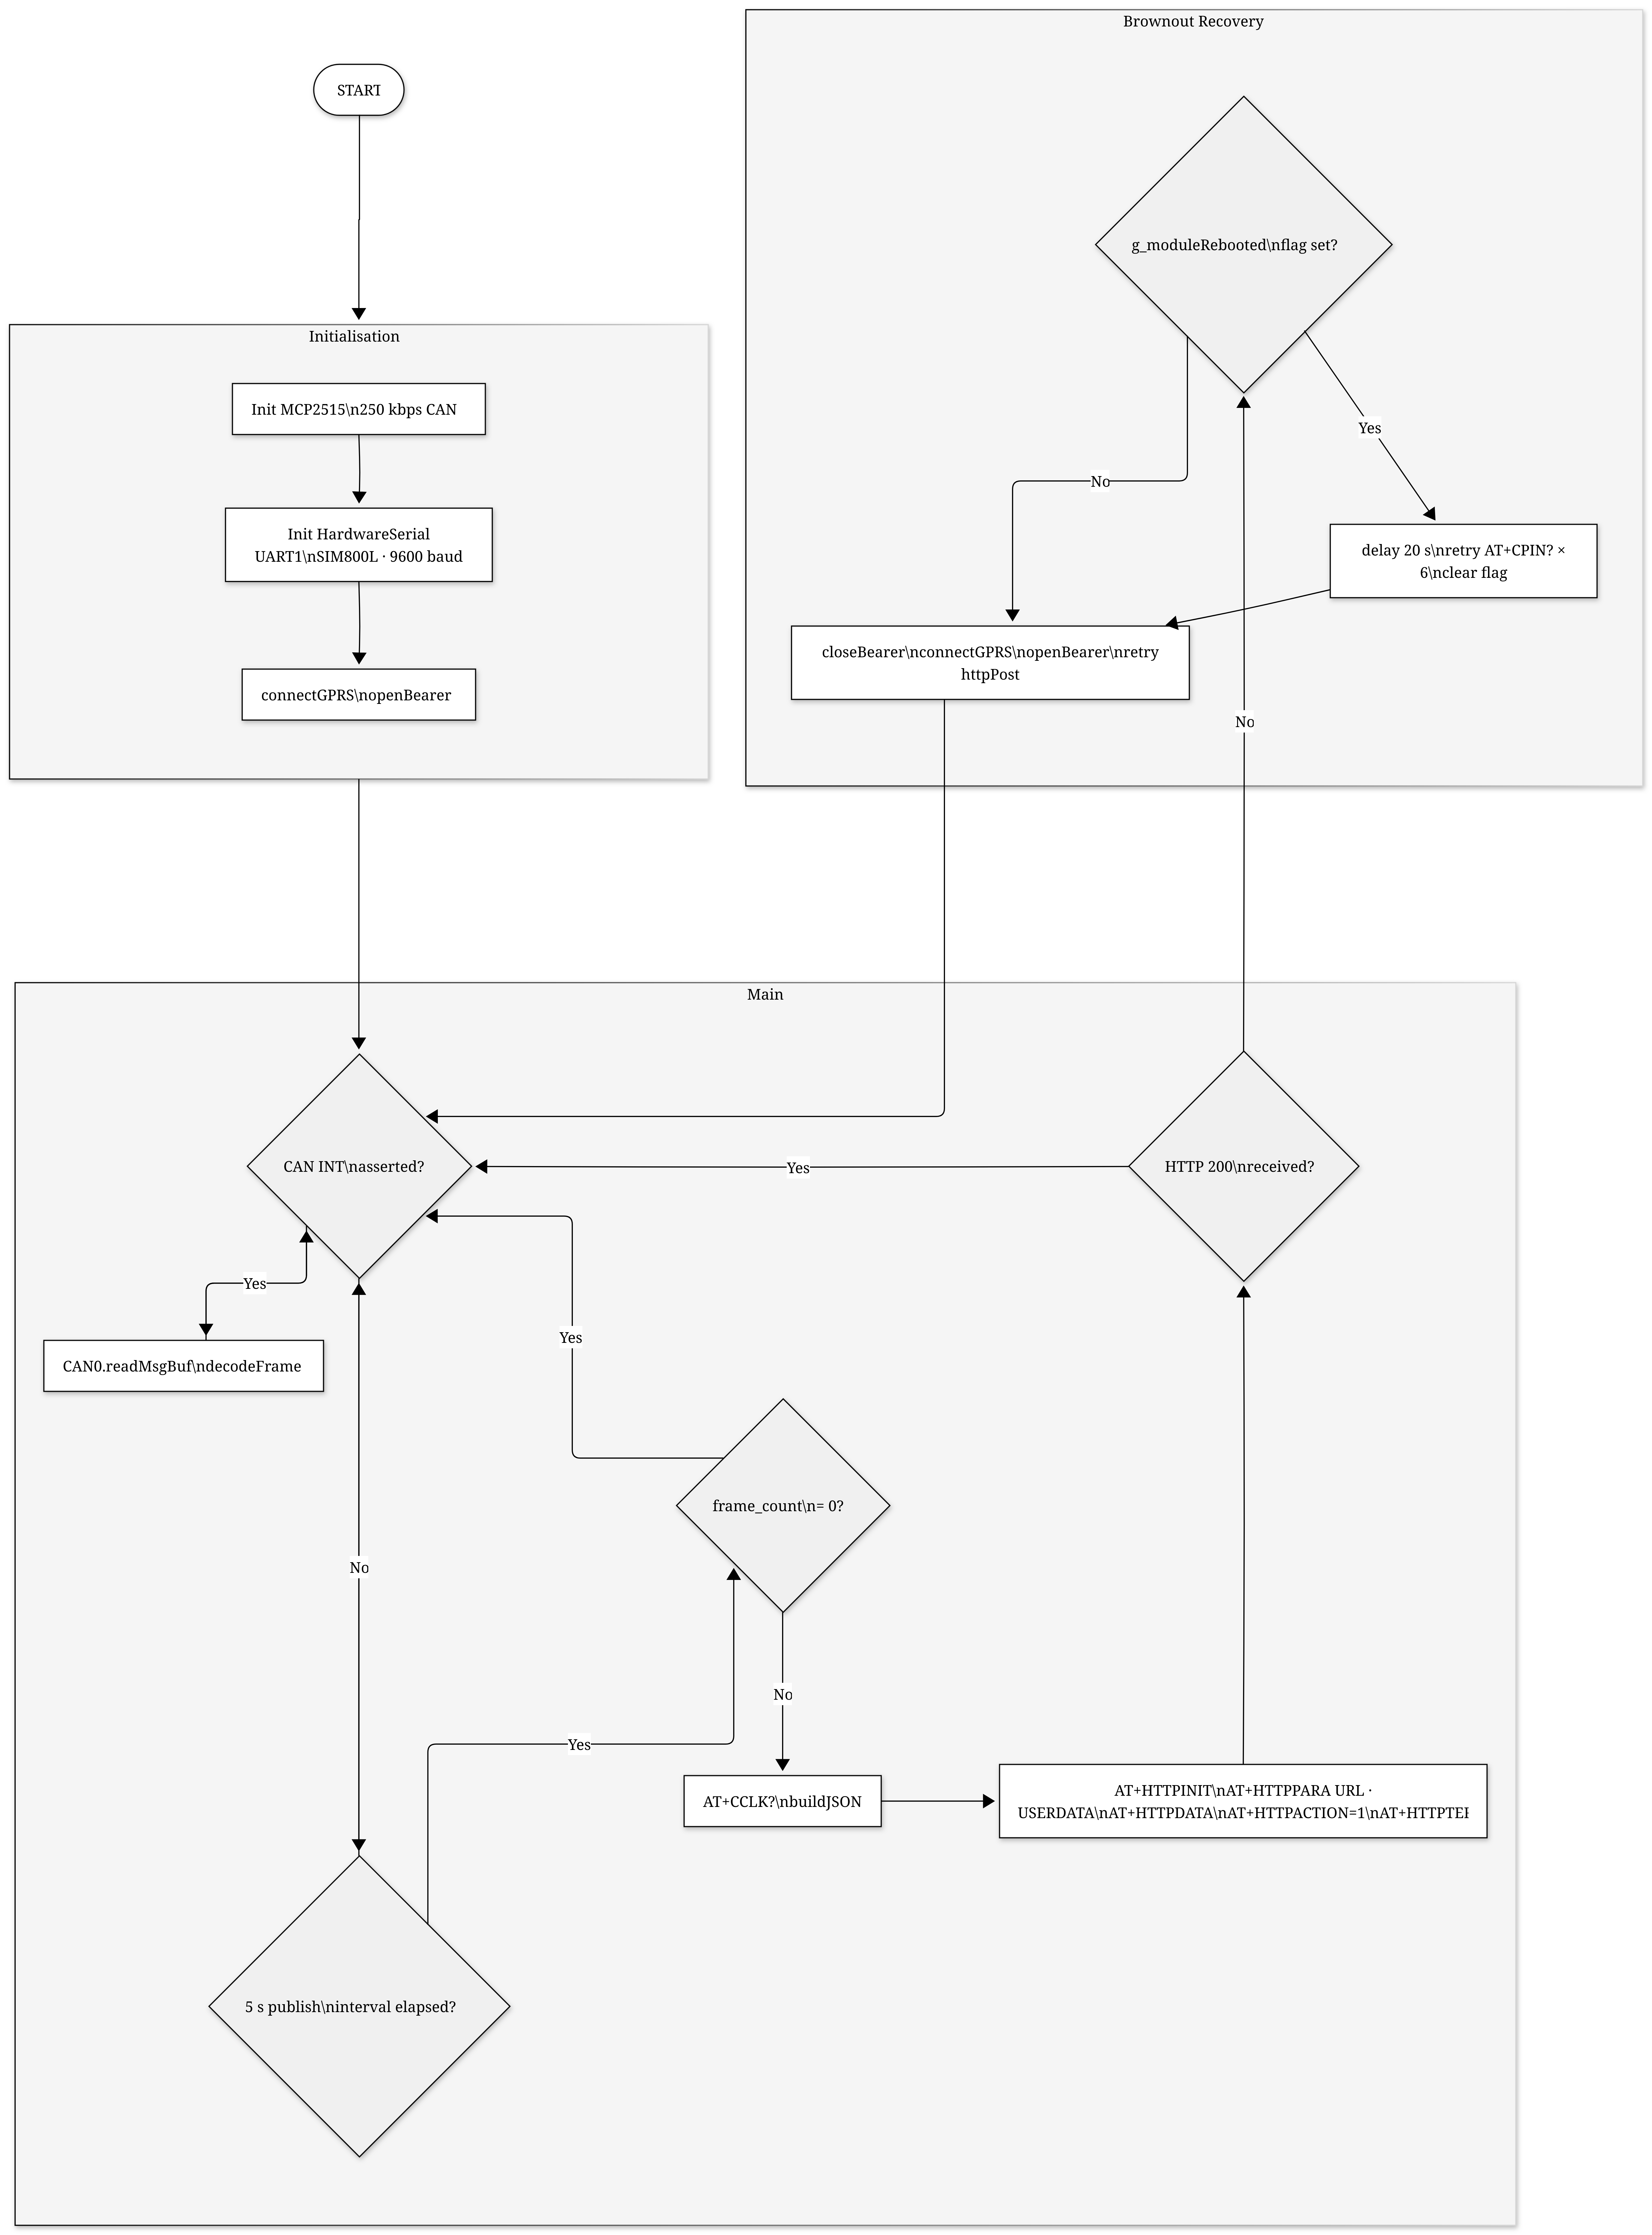
\includegraphics[width=0.7\textwidth]{images/firmware-flow-s.png}
    \caption{Firmware main-loop execution model: CAN drain $\rightarrow$ publish every 5 s}
    \label{fig:fw-flow}
\end{figure}

The SIM800L GPRS module (driven via the SIM800L AT command protocol) is connected to \textbf{HardwareSerial UART1} (GPIO 16/17) at 9600 baud. HardwareSerial was chosen over SoftwareSerial because the module's AT+HTTP* responses can arrive as multi-line bursts that SoftwareSerial's byte-at-a-time interrupt handler occasionally corrupts at 9600 baud on a loaded CPU.

% ─────────────────────────────────────────────────────────────────────────────
\subsection{BMS Firmware}
\label{sec:bms-firmware}

The BMS firmware is responsible for reading raw CAN frames from the O'CELL IFS60.8-500-F-E3 battery management system~\cite{ocellspec}, decoding them according to the \textbf{SAE J1939} standard~\cite{bakocan}, maintaining a live BMS state structure, and serializing that state to JSON for cloud upload.

\subsubsection{CAN Bus Interface}

The physical CAN interface uses a \textbf{MCP2515} controller connected to the ESP32 via the VSPI bus at 10 MHz. The bus operates at \textbf{250 kbps}, which is the standard J1939 baud rate for vehicle control networks~\cite{saej1939}. All frames from the O'CELL BMS use 29-bit extended CAN identifiers, formatted according to the J1939 Parameter Group Number (PGN) convention:

\begin{equation}
    \label{eq:j1939-id}
    \text{CAN ID} = 0x18\_\text{FUNC}\_\text{SUB}\_\text{SA}
\end{equation}

where \texttt{FUNC} is the PGN function byte that identifies the frame type, \texttt{SUB} encodes sub-addressing or destination, and \texttt{SA} = 0xF4 is the source address of the BMS module.

The MCP2515 library is configured in \texttt{MCP\_ANY} mask mode so that all frames on the bus are received without hardware fiGPRSring. Software-side fiGPRSring is performed in the \texttt{decodeFrame()} function by inspecting the \texttt{FUNC} and \texttt{SUB} bytes extracted from the 29-bit ID.

\subsubsection{Supported Frame Types}

Five distinct frame types are decoded, covering all BMS data needed for monitoring and fault diagnosis. Table~\ref{tab:can-frames} lists each frame with its CAN ID, transmission rate, and data content.

\begin{table}[h]
    \centering
    \caption{O'CELL BMS CAN Frame Map (SAE J1939, 250 kbps)}
    \label{tab:can-frames}
    \begin{tabular}{llcl}
        \toprule
        \textbf{CAN ID} & \textbf{Name} & \textbf{Rate (ms)} & \textbf{Content} \\
        \midrule
        \texttt{0x18C8--CC28F4} & Cell voltages (5 frames) & 500 & 4 cells each, big-endian uint16, 1 mV/bit \\
        \texttt{0x18B428F4}     & Temperature probes        & 500 & Up to 8 probes, raw $-$ 40 = °C \\
        \texttt{0x18FF28F4}     & BMS Basic Message 1       & 100 & SOC, current, voltage, fault flags \\
        \texttt{0x18FE28F4}     & BMS Basic Message 2       & 100 & Min/max cell mV, discharge limit \\
        \texttt{0x18FFE5F4}     & Charging request          & 500 & Max charge V, max charge A, start signal \\
        \bottomrule
    \end{tabular}
\end{table}

\paragraph{Cell Voltage Frames (0x18C8--CC28F4).}
The 19 battery cells are transmitted across five consecutive frames. Each frame carries four cells encoded as big-endian 16-bit unsigned integers, with a resolution of 1 mV per bit. The last frame (0x18CC28F4) covers cells 17--19 and pads the unused fourth slot with 0x0000. The firmware detects and skips zero-padded slots:

\begin{verbatim}
for (int i = 0; i < 4; i++) {
    uint16_t mv = u16be(data, i * 2);
    if (mv != 0 && (base + i) < 19)
        bms.cell_mv[base + i] = mv;
}
\end{verbatim}

After each group update, aggregate statistics (minimum, maximum, average) are recomputed from all non-zero cells, and a voltage-based SOC estimate is derived as described in Section~\ref{sec:soc-cal}.

\paragraph{BMS Basic Message 1 (0x18FF28F4).}
This 100 ms frame carries the core operational state of the pack. The byte layout is as follows:

\begin{itemize}
    \item \textbf{Byte 0} — Status bit-field: charge cable connected (bit 0), charging in progress (bit 1), discharging in progress (bit 2), BMS ready (bit 3), discharge contactor closed (bit 4), charge contactor closed (bit 5).
    \item \textbf{Byte 1} — State of charge from the BMS coulomb counter (0--100\%).
    \item \textbf{Bytes 2--3} — Pack current as a little-endian uint16 with a $-$5000 offset and 0.1 A/bit scaling. Positive values indicate discharge; negative values indicate charging.
    \item \textbf{Bytes 4--5} — Direct BMS pack voltage, little-endian uint16, 0.1 V/bit.
    \item \textbf{Byte 6} — Fault severity level (0 = normal, 1 = serious fault).
    \item \textbf{Byte 7} — Fault code (see Table~\ref{tab:fault-codes}).
\end{itemize}

\begin{table}[h]
    \centering
    \caption{BMS Fault Code Map (byte 7 of 0x18FF28F4)}
    \label{tab:fault-codes}
    \begin{tabular}{cl}
        \toprule
        \textbf{Code} & \textbf{Description} \\
        \midrule
        0x00 & No fault (normal operation) \\
        0x01 & Over-temperature — severe \\
        0x02 & Total pack voltage too high \\
        0x03 & Total pack voltage too low \\
        0x04 & Discharge over-current \\
        0x05 & Cell voltage too high \\
        0x06 & Cell voltage too low \\
        \bottomrule
    \end{tabular}
\end{table}

\paragraph{Temperature Probes (0x18B428F4).}
Up to eight thermal probes are encoded as single bytes using the formula $T[\text{°C}] = \text{raw} - 40$~\cite{ds18b20datasheet}. A raw value of 0xFF indicates a disconnected sensor and is skipped. The O'CELL pack fitted to the vehicle contains four active probes.

\paragraph{Charging Request (0x18FFE5F4).}
This frame is transmitted by the BMS toward the on-board charger. It specifies the maximum allowable terminal voltage (bytes 0--1, 0.1 V/bit) and maximum charge current (bytes 2--3, 0.1 A/bit). Bit 0 of byte 4 being clear signals that the BMS is requesting the charger to begin charging.

\subsubsection{BMS State Structure}

All decoded values are accumulated into a single \texttt{BMSData} struct that persists across frames and represents the most recent complete snapshot of the battery's state. The struct is updated in-place by \texttt{decodeFrame()} and read atomically by \texttt{buildJSON()} at each publish cycle. Because the firmware runs single-threaded, no locking is required.

\subsubsection{SOC Calibration}
\label{sec:soc-cal}

The firmware uses a \textbf{voltage-based SOC estimate} derived from the average cell voltage~\cite{lifepo4soc}. This method was selected because it correlates closely with the vehicle's own dashboard reading, unlike the BMS internal coulomb counter which can drift over time~\cite{bmssoc}.

The calibration was performed over four separate on-vehicle sessions, comparing the computed average cell voltage with the vehicle's onboard display:

\begin{equation}
    \label{eq:soc}
    \text{SOC} [\%] = \frac{\overline{V}_{\text{cell}} - 2500}{3387 - 2500} \times 100
\end{equation}

where $\overline{V}_{\text{cell}}$ is the average cell voltage in millivolts. The lower bound of 2500 mV/cell corresponds to 0\% SOC (47.50 V pack), and 3387 mV/cell was calibrated to match 100\% on the car display (64.35 V pack). Values above 3387 mV, which occur during active charging, are clamped to 100\%.

Table~\ref{tab:soc-cal} shows the four calibration sessions used to arrive at the 3387 mV reference point.

\begin{table}[h]
    \centering
    \caption{SOC Calibration Data — Four On-Vehicle Sessions}
    \label{tab:soc-cal}
    \begin{tabular}{cccc}
        \toprule
        \textbf{Session} & \textbf{Avg cell (mV)} & \textbf{Car display (\%)} & \textbf{Solved top (mV)} \\
        \midrule
        2026-03-31 10:06 & 3301.6 & 89.0 & 3400.7 \\
        2026-03-31 10:57 & 3306.2 & 89.0 & 3405.8 \\
        2026-04-01 13:03 & 3284.8 & 89.4 & 3377.9 \\
        2026-04-01 16:04 & 3285.0 & 88.4 & 3387.4 \\
        \midrule
        \multicolumn{3}{r}{\textbf{Adopted reference}} & \textbf{3387 mV} \\
        \bottomrule
    \end{tabular}
\end{table}

\subsubsection{Cloud Publishing via SIM800L}

At every 5-second publish interval, the firmware calls \texttt{buildJSON()} to serialize the current \texttt{BMSData} struct into a nested JSON document using the ArduinoJson v7 library~\cite{arduinojson}, then calls \texttt{httpPost()} to deliver it to the VPS backend via SIM800L GPRS.

The payload uses a five-section nested schema: a top-level envelope wraps \texttt{battery}, \texttt{temperatures}, \texttt{solar}, \texttt{dc\_dc}, and \texttt{vehicle} sub-objects. Individual cell voltages are encoded as a 1-based JSON array (\texttt{cells[0] = null}, \texttt{cells[1]\ldots cells[19] = \{mv, status\}}). Temperature probes follow the same convention in \texttt{temperatures.battery\_cells}. Sensors not yet instrumented (solar, DC/DC, vehicle) appear as \texttt{null}-valued fields so the schema remains stable as additional sensors are commissioned.

The HTTP transaction uses the SIM800L's native \textbf{AT+HTTP*} command set over plain HTTP (AT+HTTPSSL=0). The sequence is:

\begin{enumerate}
    \item \texttt{AT+HTTPTERM} — close any stale session from a previous transaction.
    \item \texttt{AT+HTTPINIT} — open a new HTTP session.
    \item \texttt{AT+HTTPPARA="URL",...} — set the full endpoint URL.
    \item \texttt{AT+HTTPPARA="USERDATA","X-Api-Key: \textit{key}\textbackslash r\textbackslash n"} — inject the API authentication header.
    \item \texttt{AT+HTTPDATA=\textit{len},10000} — upload the JSON body.
    \item \texttt{AT+HTTPACTION=1} — execute the HTTP POST and wait for \texttt{+HTTPACTION:} response.
    \item \texttt{AT+HTTPTERM} — close the session.
\end{enumerate}

During the AT+HTTPACTION wait loop (up to 30 s), the firmware continues draining CAN frames from the MCP2515 receive buffer so that no BMS data is lost while the module is busy.

\subsubsection{Brownout Recovery}

A known failure mode of the SIM800L is a mid-transaction power brownout caused by the $\sim$1.5 A peak current during GPRS transmission exceeding the supply rail's transient capability. When this occurs, the module resets and emits an unsolicited \texttt{"Call Ready"} string in its UART output.

The firmware detects this string in all three response handlers: \texttt{sendAT()}, \texttt{sendATExpect()}, and the \texttt{HTTPACTION} wait loop and sets a global \texttt{g\_moduleRebooted} flag. When a publish cycle fails and this flag is set, the recovery sequence is:

\begin{enumerate}
    \item Wait 20 s for the SIM card and GPRS stack to re-initialize.
    \item Retry \texttt{AT+CPIN?} up to six times at 4-second intervals.
    \item Re-open the GPRS bearer and retry the publish once more.
\end{enumerate}

The hardware fix is to add a 2200~\textmu{}F / 6.3~V bulk capacitor close to the module VBAT pin, as incorporated into PCB Revision RECTIFICATION\_2.

% ─────────────────────────────────────────────────────────────────────────────
\subsection{CAN Frame Parser}
\label{sec:can-frame-parser}

The \texttt{parse\_can()} function in the Python backend implements the BAKO CAN Protocol Rev~1.0, decoding all frames broadcast by the BMS (SA = 0xF4) and all sensor gateway frames transmitted by the ESP32 (SA = 0xAA). A companion \texttt{parse\_sensor()} function handles the \texttt{SENSOR:} text-line fallback format emitted by the Python simulator.

\subsubsection{BMS Frames (SA = 0xF4)}

Table~\ref{tab:can-parser-bms} lists all five BMS frame types decoded by \texttt{parse\_can()}, with their CAN IDs, transmission cycles, decoded fields, and key decoding logic.

\begin{table}[H]
\centering
\caption{BMS CAN Frame Parser --- SA = 0xF4 (O'CELL BMS)}
\label{tab:can-parser-bms}
\small
\begin{tabular}{>{\ttfamily}p{3.5cm} c p{4.5cm} p{4.0cm}}
\toprule
\textbf{CAN ID} & \textbf{Cycle} & \textbf{Fields decoded} & \textbf{Key decoding logic} \\
\midrule
0x18FF28F4 & 100 ms & SOC\%, pack current, pack voltage, fault level, error code & Pack current: (uint16\_LE $-$ 5000) $\times$ 0.1~A; Pack voltage: uint16\_LE $\times$ 0.1~V \\
\midrule
0x18FE28F4 & 100 ms & Max/min cell voltage, max/min temp, max discharge current & Temperatures: uint8 $-$ 40~°C; 0xFF = not connected \\
\midrule
0x18C8--CC28F4 & 500 ms & All 19 cell voltages (4 per frame) & Big-endian uint16 mV pairs; PF byte determines group index (0xC8 = group 0 $\rightarrow$ cells 1--4) \\
\midrule
0x18B428F4 & 500 ms & Up to 8 temperature probe values & uint8 offset $-$40~°C; 0xFF = probe not connected \\
\midrule
0x18FFE5F4 & 1000 ms & Max charge voltage, max charge current & uint16\_LE $\times$ 0.1~V / 0.1~A \\
\bottomrule
\end{tabular}
\end{table}

\subsubsection{ESP32 Sensor Gateway Frames (SA = 0xAA)}

In addition to receiving BMS frames, the ESP32 re-broadcasts external sensor readings as J1939-formatted CAN frames using its own source address (SA = 0xAA). This allows any device on the bus to consume solar, MPPT, thermal, and vehicle state data using a standard CAN interface. Table~\ref{tab:can-parser-esp32} lists all eight gateway frame types.

\begin{table}[H]
\centering
\caption{ESP32 Sensor Gateway CAN Frame Map --- SA = 0xAA}
\label{tab:can-parser-esp32}
\small
\begin{tabular}{>{\ttfamily}p{3.2cm} c p{8.0cm}}
\toprule
\textbf{CAN ID} & \textbf{Cycle} & \textbf{Content} \\
\midrule
0x18D001AA & 200 ms & Solar panel current before MPPT — raw + 5-cycle average (uint16\_LE $\times$ 0.1~A) \\
0x18D101AA & 200 ms & Solar panel voltage + open-circuit $V_{oc}$ (uint16\_LE $\times$ 0.1~V) \\
0x18D201AA & 200 ms & MPPT output current + mode (0=off / 1=track / 2=CV / 3=float) + efficiency~\% \\
0x18D301AA & 200 ms & DC/DC 12~V output voltage ($\times$~0.01~V) + current ($\times$~0.1~A; 0xFFFF = not fitted) \\
0x18D401AA & 1000 ms & Motor temperature (uint8 $-$ 40~°C) \\
0x18D501AA & 1000 ms & MPPT heatsink temperature (uint8 $-$ 40~°C) \\
0x18D601AA & 1000 ms & DC/DC heatsink temperature (uint8 $-$ 40~°C) \\
0x18D701AA & 500 ms & Handbrake position: 0 = released, 1 = engaged, 0xFF = sensor fault; + debounce flag \\
0x18D801AA & 500 ms & GNSS information (position, speed, heading) \\
\bottomrule
\end{tabular}
\end{table}

\subsubsection{SOC Representations and SOH Calculation}

Three distinct SOC representations are maintained simultaneously by the parser:

\begin{description}
    \item[\texttt{soc\_bms}] Raw coulomb-counter value from byte~2 of 0x18FF28F4. Directly reported by the BMS hardware; prone to drift over long charge/discharge cycles.

    \item[\texttt{soc}] Voltage-based SOC derived from the average cell voltage using the calibrated formula (Equation~\ref{eq:soc}):
    \[
        \text{SOC} = \frac{\overline{V}_{\text{cell}} - 2500}{3387 - 2500} \times 100, \quad \text{clamped to } [0, 100]\%
    \]
    The upper reference (3387~mV) was calibrated from four real vehicle logs. This is the primary value displayed on the dashboard.

    \item[\texttt{soc\_coulomb}] Charge request signal derived from 0x18FFE5F4 (the charging request frame), used for charger control decisions. The frame carries the BMS-requested maximum charge voltage and current; its \texttt{start\_signal} bit is monitored to track active charging state.
\end{description}

State of Health (SoH) is calculated from the ratio of the measured actual capacity to the rated pack capacity:
\[
    \text{SoH} = \frac{C_{\text{actual}}}{C_{\text{rated}}} \times 100 = \frac{44.7}{50.0} \times 100 = 89.4\%
\]

% ─────────────────────────────────────────────────────────────────────────────
\subsection{Motor Control Algorithms}

Motor control algorithms are outside the scope of this monitoring system. The ESP32 firmware reads and monitors motor-related sensor data --- specifically motor temperature via DS18B20 and current draw via the ACS712/ACS758 sensors --- but does not interface with the motor controller or implement any drive control logic. Motor speed and torque management remain the responsibility of the existing vehicle control electronics. This boundary is intentional: the monitoring system observes and reports motor operating conditions without intervening in the drivetrain control loop.

% ─────────────────────────────────────────────────────────────────────────────
\subsection{Vehicle Management Unit (VMU) Software}

The Vehicle Management Unit (VMU) is implemented on the same ESP32 microcontroller and is responsible for the higher-level coordination layer above raw sensor acquisition. Specifically, the VMU software handles four functions:

\begin{description}
    \item[\textbf{Data aggregation}] Collecting decoded CAN frames from the BMS (cell voltages, SOC, pack current, temperatures, and fault flags) together with readings from external sensors (DC/DC voltage, MPPT current, motor temperature, and handbrake position) into a unified telemetry structure.

    \item[\textbf{Data formatting}] Structuring all acquired telemetry into a consistent JSON schema for transmission to the dashboard over WebSocket or to the cloud back-end via the SIM800L GSM/GPRS module.

    \item[\textbf{Communication management}] Switching between Wi-Fi Access Point mode (for local dashboard access) and Serial mode (for USB-connected debugging and development), based on the firmware build configuration.

    \item[\textbf{Alert handling}] Monitoring configured thresholds --- including over-temperature limits for the motor and DC/DC converter, battery fault flags from the BMS, and handbrake engagement --- and updating the status LED outputs and dashboard warning panels accordingly.
\end{description}

The VMU software does not perform low-level motor control or BMS internal management; it only reads data from those systems and presents it to the operator.

% ─────────────────────────────────────────────────────────────────────────────
\subsection{ESP32 Access Point Mode}

The ESP32 operates in \textbf{Wi-Fi Access Point (AP) mode} for local dashboard access, having been migrated from an earlier Station Mode implementation. The ESP32 chip supports two distinct Wi-Fi operating modes: Station Mode (STA), where it joins an existing router and receives a DHCP-assigned IP; and Access Point Mode (AP), where it becomes the router, broadcasts its own SSID, and assigns addresses to connecting devices with no external router required.

\subsubsection*{Why Station Mode Was Replaced}

The original firmware connected the ESP32 to a home Wi-Fi router as a station. This introduced three practical drawbacks: the SSID and password were hardcoded, so using the system in a different location required reflashing; the router's DHCP server assigned a different IP address after every reboot, requiring firmware updates to match the PC's current address; and without a nearby router, the simulation environment required a mobile hotspot workaround that added extra configuration steps. AP mode resolves all three issues: the ESP32 brings its own network, the IP address 192.168.4.1 never changes, and the system operates in any location without code changes.

\subsubsection*{AP Mode Internal Operation}

When \texttt{WiFi.softAP()} is called, the ESP32 radio switches to infrastructure mode. The built-in DHCP server listens on 192.168.4.1 and issues leases from the pool 192.168.4.2--192.168.4.11. The application code opens a \texttt{WiFiServer} on port 9000. When a client connects to 192.168.4.1:9000, the lwIP stack completes the TCP three-way handshake and places the connection in the accept queue for the firmware to service.

\subsubsection*{Firmware Changes}

The migration from Station to AP mode required minimal changes, isolated entirely to the Wi-Fi and TCP layer. The simulation engine, phase logic, frame encoders, and timing are identical to the station-mode version. The key changes were:

\begin{itemize}
    \item \textbf{Removed:} \texttt{WIFI\_SSID}, \texttt{WIFI\_PASS}, \texttt{SERVER\_IP} constants; \texttt{ensureWiFi()} and \texttt{ensureTCP()} functions.
    \item \textbf{Added:} \texttt{AP\_SSID}, \texttt{AP\_PASS}, \texttt{AP\_CHANNEL} constants; \texttt{WiFiServer server(TCP\_PORT)} global; \texttt{startAP()} and \texttt{ensureClient()} functions.
    \item \texttt{setup()} now calls \texttt{startAP()} and \texttt{server.begin()} instead of \texttt{ensureWiFi()} and \texttt{ensureTCP()}.
    \item \texttt{loop()} calls \texttt{ensureClient()} with a 50~ms yield when no client is connected, keeping the DHCP and beacon tasks running without burning CPU.
\end{itemize}

The \texttt{server.py} dashboard application required zero modifications. It accepts connections on any local interface, including the 192.168.4.x interface created when the PC joins the BAKO\_SMU network. The only operational change for the user is connecting the PC to the \texttt{BAKO\_BMS} Wi-Fi network before launching the server.

% ─────────────────────────────────────────────────────────────────────────────
\subsection{OTA Firmware Updates \& Web Configuration Portal}
\label{sec:ota}

This section documents the third and final stage of the Wi-Fi connectivity evolution. Following the migration from Station Mode to Access Point (AP) Mode, two complementary features were added: Over-The-Air (OTA) firmware flashing and a browser-based configuration portal. Together they make the system fully maintainable in the field without physical access to the PCB.

\subsubsection*{Development Progression Summary}

The connectivity stack evolved through three clearly defined stages. Table~\ref{tab:wifi-evolution} summarises each stage, its purpose, and the limitation that motivated the next iteration.

\begin{table}[H]
\centering
\caption{Wi-Fi Connectivity Evolution Across Three Development Stages}
\label{tab:wifi-evolution}
\small
\begin{tabular}{c >{\bfseries}p{2.5cm} p{4.5cm} p{4.5cm}}
\toprule
\textbf{Stage} & \textbf{Mode} & \textbf{What was achieved} & \textbf{Limitation that led to next stage} \\
\midrule
1 & Station Mode (STA) & ESP32 joins existing Wi-Fi router. DHCP-assigned IP. Dashboard PC on same LAN. & Router dependency, dynamic IP, hardcoded SSID/password in firmware. \\
\midrule
2 & Access Point Mode (AP) & ESP32 is its own router. Fixed IP 192.168.4.1. No external network needed. & Reflashing still required USB cable. Network parameters hardcoded. \\
\midrule
3 & AP + OTA + Web Config & Wireless firmware flashing from IDE. Browser portal to change all network settings without reflashing. & No further limitation — system is fully field-maintainable. \\
\bottomrule
\end{tabular}
\end{table}

\subsubsection*{Over-The-Air Firmware Update}

The \textbf{ArduinoOTA} library was integrated into the ESP32 firmware to allow wireless firmware flashing directly from the Arduino IDE over the existing AP network. The OTA service runs as a lightweight background handler (\texttt{ArduinoOTA.handle()}) called at every loop iteration alongside the TCP and web servers, adding negligible overhead.

\paragraph{Motivation.}
Once the PCB is mounted inside a vehicle enclosure, accessing the USB port for reflashing is impractical. OTA eliminates this constraint: the technician connects a laptop to the \texttt{BAKO\_BMS} Wi-Fi network, selects the network port in the IDE, and clicks Upload — the new firmware is transmitted wirelessly, verified, and applied.

\paragraph{OTA flashing procedure.}
\begin{enumerate}
    \item Power the ESP32 board (vehicle on, or bench supply connected).
    \item Connect the laptop to the \texttt{BAKO\_BMS} Wi-Fi network broadcast by the ESP32.
    \item Open Arduino IDE → Tools → Port. A network port labelled with the OTA hostname (\texttt{BAKO\_OTA} by default) appears automatically.
    \item Select that port, compile, and click \textbf{Upload} as normal.
    \item The IDE transmits the binary wirelessly. The ESP32 verifies integrity and reboots into the new firmware.
\end{enumerate}

\paragraph{Security.}
The OTA service is password-protected to prevent unauthorised firmware injection. The password is configurable through the web portal and stored in NVS flash so it survives reboots. If an active TCP dashboard client is connected when an OTA session begins, the client socket is cleanly closed before flashing starts to prevent data corruption.

\subsubsection*{Web Configuration Portal}

To avoid hardcoding network parameters into the firmware — which would require a reflash every time the AP name, channel, TCP port, or OTA credentials needed changing — a browser-based configuration portal was implemented and served directly by the ESP32 on port~80 using the \textbf{WebServer} library.

The portal is accessible at \texttt{http://192.168.4.1} from any device connected to the ESP32's AP network. It is styled with the BAKO green colour scheme and renders correctly on both desktop browsers and mobile devices.

\begin{figure}[H]
    \centering
    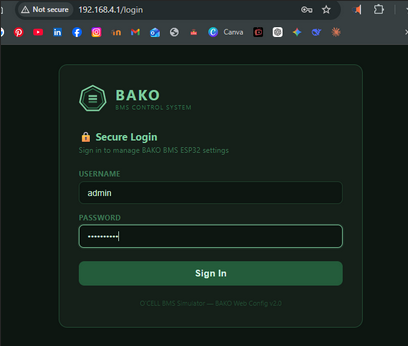
\includegraphics[width=0.55\textwidth]{images/portal-login.png}
    \caption{BAKO BMS web portal login page --- accessible from any browser on the AP network at \texttt{http://192.168.4.1/login}.}
    \label{fig:portal-login}
\end{figure}

After successful login, the operator is directed to the configuration form at \texttt{/config}. Table~\ref{tab:portal-params} lists all configurable parameters.

\begin{table}[H]
\centering
\caption{Configurable Parameters Exposed Through the BAKO Web Portal}
\label{tab:portal-params}
\small
\begin{tabular}{>{\bfseries}p{2.8cm} p{2.5cm} p{7.5cm}}
\toprule
Parameter & Default & Description \\
\midrule
AP SSID        & \texttt{BAKO\_BMS}  & Wi-Fi network name broadcast by the ESP32. \\
AP Password    & \texttt{12345678}   & Minimum 8 characters; leave blank for an open network. \\
WiFi Channel   & \texttt{6}          & Selectable 1--13 to avoid interference with nearby networks. \\
TCP Port       & \texttt{9000}       & Port the Python dashboard server connects to. \\
OTA Hostname   & \texttt{BAKO\_OTA}  & Name visible in Arduino IDE → Tools → Port for OTA flashing. \\
OTA Password   & \texttt{12345678}   & Protects the OTA endpoint against unauthorised firmware injection. \\
\bottomrule
\end{tabular}
\end{table}

\begin{figure}[H]
    \centering
    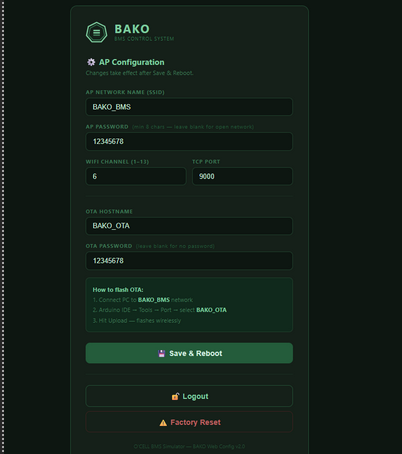
\includegraphics[width=0.55\textwidth]{images/portal-config.png}
    \caption{Web configuration portal --- AP Configuration page showing SSID, password, Wi-Fi channel, TCP port, OTA hostname, and OTA password fields.}
    \label{fig:portal-config}
\end{figure}

\subsubsection*{Web Portal Route Map}

The web server runs on port~80 and handles the following routes. All routes except \texttt{/login} redirect to \texttt{/login} if no valid session cookie is present.

\begin{table}[H]
\centering
\caption{Web Portal Route Map --- All Routes Protected by Session Authentication}
\label{tab:portal-routes}
\small
\begin{tabular}{>{\ttfamily}p{2.8cm} p{2.0cm} p{8.0cm}}
\toprule
\textbf{Route} & \textbf{Method} & \textbf{Function} \\
\midrule
/              & GET        & Redirects to \texttt{/config} if session valid, otherwise to \texttt{/login}. \\
/login         & GET / POST & GET: renders login form. POST: validates credentials; on success sets session cookie and redirects to \texttt{/config}. \\
/config        & GET / POST & GET: renders configuration form (auth required). POST: validates and saves settings, triggers reboot. \\
/logout        & POST       & Invalidates the session token and redirects to \texttt{/login}. \\
/factoryreset  & POST       & Clears all NVS settings and reboots to defaults (auth required). Separate POST-only route prevents accidental GET trigger. \\
\bottomrule
\end{tabular}
\end{table}

\subsubsection*{Simultaneous Services on the ESP32}

After Stage~3 integration, the ESP32 operates four network services concurrently from a single \texttt{loop()} function without measurable impact on CAN frame timing or dashboard refresh rate.

\begin{table}[H]
\centering
\caption{Four Network Services Running Simultaneously on the ESP32 After Stage~3 Integration}
\label{tab:esp32-services}
\small
\begin{tabular}{>{\bfseries}p{3.0cm} p{1.5cm} p{3.0cm} p{5.0cm}}
\toprule
Service & Port & Handler in \texttt{loop()} & Purpose \\
\midrule
Wi-Fi Access Point  & N/A (radio)    & \texttt{WiFi.softAP()} (setup only)  & Broadcasts SSID, runs DHCP, assigns 192.168.4.x addresses. \\
TCP CAN data server & 9000 (default) & \texttt{ensureClient()}               & Streams live CAN frames to the Python dashboard server. \\
OTA update service  & 8266 (mDNS)    & \texttt{ArduinoOTA.handle()}          & Accepts wireless firmware uploads from Arduino IDE. \\
HTTP web config portal & 80          & \texttt{webServer.handleClient()}     & Serves login \& config pages for changing all network settings. \\
\bottomrule
\end{tabular}
\end{table}

% ─────────────────────────────────────────────────────────────────────────────
\subsection{Unit \& Integration Testing}

Software testing for the BMS firmware and cloud pipeline was conducted at three levels: unit testing of the decoding logic, integration testing of the full CAN-to-cloud pipeline, and functional testing of the live dashboard.

\subsubsection{Unit Testing — Frame Decoder}

Each frame type in \texttt{decodeFrame()} was verified by replaying known raw bytes and checking the decoded output against hand-computed expected values. The test case below illustrates verification of cell voltage frame 0x18CB28F4:

\begin{verbatim}
Frame ID: 0x18CB28F4   Data: 0D 3F  0D 38  0D 3A  0D 39

0x0D3F = 3391 mV  -> Cell 13   (big-endian, group = 0xCB - 0xC8 = 3)
0x0D38 = 3384 mV  -> Cell 14
0x0D3A = 3386 mV  -> Cell 15
0x0D39 = 3385 mV  -> Cell 16
\end{verbatim}

Similarly, the signed current decoding formula (offset $-$5000, scale 0.1 A/bit) and the SOC formula (Equation~\eqref{eq:soc}) were verified against values from the real car log file \texttt{bms\_log\_2026-03-10T10-20-02.txt}, which contains 3197 frames captured during an on-vehicle session.

\subsubsection{Integration Testing — Cloud Pipeline}

The end-to-end pipeline was tested without live hardware using the \texttt{replay\_to\_cloud.py} tool, which parses the captured CAN log and replays decoded JSON snapshots to \texttt{POST /api/ingest} at configurable speed. This allowed the following verifications:

\begin{itemize}
    \item The \texttt{/api/ingest} endpoint correctly rejects requests with an invalid \texttt{X-Api-Key} header (HTTP 401).
    \item Each accepted snapshot is stored in the SQLite \texttt{bms\_cloud.db} database with correct timestamp and device ID.
    \item The \texttt{/ws/cloud} WebSocket pushes the most recent snapshot to all connected browser clients within 2 seconds of ingestion.
    \item The \texttt{/api/history} endpoint returns records newest-first with correct JSON structure.
\end{itemize}

\subsubsection{Functional Testing — Live Dashboard}

The live dashboard (\texttt{frontend/index.html}) was tested in both SERIAL and CLOUD modes:

\begin{description}
    \item[SERIAL mode] ESP32 connected via USB to a development laptop. The server decoded incoming frames in real time and the 19-cell voltage grid, SOC ring, and temperature bars updated at 10 Hz without visible lag.
    \item[CLOUD mode] Data replayed from the log file through \texttt{/api/ingest}. The dashboard received snapshots via \texttt{/ws/cloud} at 2 Hz and all panels rendered correctly, including the cloud communication log panel which displayed timestamped RECV and WS events.
    \item[Reconnect behavior] The backend was deliberately stopped while the dashboard was open. The browser WebSocket closed, the connection status indicator turned red (Disconnected), and the overlay appeared. On server restart, the client automatically reconnected within 5 seconds and resumed live updates.
\end{description}

% ─────────────────────────────────────────────────────────────────────────────
\subsection{Web Dashboard}

The BAKO DIAGNOSTICS web dashboard is a dark-theme, single-page web application that provides a real-time overview of the entire vehicle monitoring state. It is served by the FastAPI back-end at the root URL (\texttt{/}) and communicates with the server via WebSocket (\texttt{/ws} in serial mode, \texttt{/ws/cloud} in cloud mode). The dashboard requires no installation; any browser that connects to the server IP receives the complete HTML, CSS, and JavaScript in a single response.

\begin{figure}[H]
    \centering
    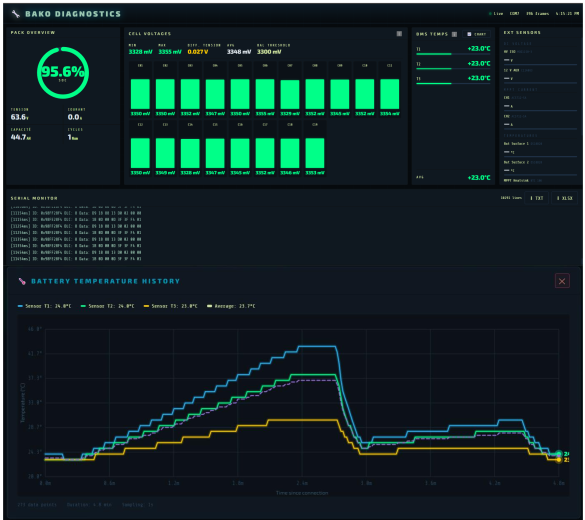
\includegraphics[width=\textwidth]{images/dashboard-screenshot.png}
    \caption{BAKO DIAGNOSTICS live dashboard --- dark-theme single-page interface showing SOC ring gauge, 19-cell voltage grid, temperature time-series chart, and external sensor panel.}
    \label{fig:dashboard-screenshot}
\end{figure}

\subsubsection*{Panel Layout}

The dashboard is organised into four panels arranged to give the engineer an at-a-glance view of all monitored subsystems. Table~\ref{tab:dashboard-panels} describes the content of each panel.

\begin{table}[H]
\centering
\caption{Dashboard Panel Layout}
\label{tab:dashboard-panels}
\small
\begin{tabular}{>{\bfseries}p{3.2cm} p{10.0cm}}
\toprule
Panel & Content \\
\midrule
Left panel &
  State of charge large ring gauge (colour-coded: green $>$30\%, orange 15--30\%, red $<$15\%); pack voltage (V); pack current (A, signed); remaining capacity (Ah); State of Health (SoH) indicator. \\
\midrule
Central panel &
  Individual cell voltage bars for all 19 cells with per-cell colour coding (overvoltage / full / balanced / nominal / low / undervoltage); minimum, maximum, and average cell voltage; cell spread indicator (max $-$ min, mV). \\
\midrule
Temperature panel &
  Four BMS internal temperature probe readings with individual bars; rolling average value; high-temperature threshold alert line. \\
\midrule
Temperature chart &
  Time-series line chart displaying the four individual probe temperatures and their rolling average scrolling in real time. \\
\midrule
Right panel &
  Extended sensor readings: solar panel voltage and current, MPPT output current, MPPT mode and efficiency, DC/DC 12~V output, motor temperature, MPPT heatsink temperature, handbrake status. \\
\midrule
Serial monitor &
  Live scrolling log of raw CAN frames and \texttt{SENSOR:} lines as received from the ESP32. \\
\midrule
File export &
  Export full session log as \texttt{.TXT} or \texttt{.XLSX} with timestamp column. \\
\bottomrule
\end{tabular}
\end{table}

\subsubsection*{Threshold Colour Coding}

Cell voltage bars transition through three colour states based on configurable per-cell thresholds: green when the cell is within its normal operating band (2900--3450~mV for LiFePO4), orange when the cell approaches either end of its safe range, and red when a threshold breach is detected. The SOC ring applies the same three-state scheme based on the pack-level SOC percentage. These thresholds are defined as JavaScript constants in \texttt{frontend/index.html} and can be adjusted without modifying the back-end.

\subsubsection*{Data Export}

The dashboard includes a \textbf{Download CSV} button that retrieves the last 100 snapshots from \texttt{/api/history} and writes them to a timestamped \texttt{.csv} file. The export covers all 19 cell voltages, all four temperature probes, pack SOC, pack voltage, pack current, and extended sensor readings in a single flat row per snapshot, suitable for import into spreadsheet or data analysis tools.

\subsubsection*{Mode Selector}

A mode pill in the dashboard header opens a modal dialog that lets the operator switch the active data source between Serial and Wi-Fi AP modes at runtime, without restarting the server. The mode selection is sent via \texttt{POST /api/mode} and persisted to \texttt{mode\_config.json} so that it is automatically restored on the next server launch.

\begin{itemize}
    \item \textbf{Serial mode} --- auto-detects the connected ESP32 USB port, or accepts manual port entry with a configurable baud rate. The server reads newline-delimited CAN frames from the serial stream.
    \item \textbf{Wi-Fi mode} --- the operator enters the ESP32 IP address (default 192.168.4.1) and TCP port (default 9000), then clicks Apply. The PC must already be connected to the \texttt{BAKO\_BMS} Wi-Fi network.
\end{itemize}

\begin{figure}[H]
    \centering
    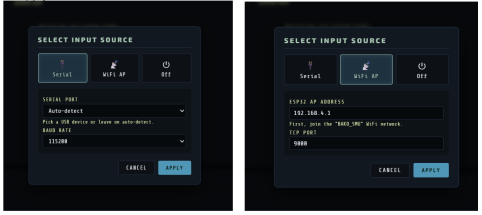
\includegraphics[width=0.85\textwidth]{images/mode-selector.png}
    \caption{Dashboard mode selector dialog: Serial mode (left) and Wi-Fi AP mode (right). Mode is switched without restarting the server.}
    \label{fig:mode-selector}
\end{figure}

% ─────────────────────────────────────────────────────────────────────────────
\subsection{Simulation \& Emulation}

Two complementary simulation tools were developed to enable dashboard testing and firmware validation without requiring a live vehicle or a real O'CELL BMS. Both tools produce data that is indistinguishable from real hardware at the server API level.

\subsubsection*{ESP32 CAN Frame Simulator}

The firmware file \texttt{CAN\_simulation\_7\_phases/CAN\_simulation\_7\_phases.ino} runs on a standalone ESP32 and generates a complete stream of realistic O'CELL BMS CAN frames over USB Serial at 115200 baud, in the same \texttt{[Xms] ID: 0x... DLC: N Data: ...} format that the real vehicle produces.

The simulator models a full charge/discharge lifecycle across seven sequential phases. Table~\ref{tab:sim-phases} describes each phase and its duration.

\begin{table}[H]
\centering
\caption{ESP32 CAN Simulator --- 7-Phase Scenario Cycle}
\label{tab:sim-phases}
\small
\begin{tabular}{c >{\bfseries}p{3.5cm} r p{6.0cm}}
\toprule
Phase & Name & Duration & Description \\
\midrule
0 & REST             & 20~s  & Pack idle at $\approx$72\% SOC; cells balanced; ambient temperature ($\approx$24\textdegree{}C). \\
1 & BULK DISCHARGE   & 120~s & 38~A load; SOC falls 72\%$\to$30\%; temperatures climb; weak cells 7 and 14 develop 15~mV extra sag. \\
2 & LOW SOC WARNING  & 25~s  & BMS throttles current 38~A$\to$12~A; SOC 30\%$\to$18\%; discharge limit ramps down to 15~A. \\
3 & RECOVERY / REST  & 15~s  & Load removed; voltage bounce-back; temperatures plateau. \\
4 & CC CHARGE        & 90~s  & 22~A constant-current charge; SOC climbs 18\%$\to$80\%; cells re-balance. \\
5 & CV TAPER         & 40~s  & Pack near full; charge current tapers 22~A$\to$2~A; spread narrows. \\
6 & FULL REST        & 20~s  & SOC 100\%; zero charge current; cells balanced ($\leq$8~mV spread); loop restarts. \\
\bottomrule
\end{tabular}
\end{table}

Each of the 19 cells has a fixed personality offset ($-20$~mV to $+12$~mV) so the cell spread is realistic and stable across frames. Cells 7 and 14 carry an additional $-18$~mV offset and a load-proportional extra sag, simulating weak cells that would trigger a threshold alert during heavy discharge. The thermal model tracks three sensors at different positions (centre, end-plate, BMS PCB) with individual heating and cooling rates. All six frame types are emitted every 500~ms: cell voltage groups (0x18C8--CC28F4), temperature (0x18B428F4), Basic Message~1 (0x18FF28F4), Basic Message~2 (0x18FE28F4), and charging request (0x18FFE5F4).

\subsubsection{ESP32 Firmware Simulator \& System Interface}

An ESP32-based firmware simulator and monitoring interface were developed to validate the BAKO system without requiring the physical vehicle during each testing session. The simulator reproduces realistic vehicle behaviour by generating sensor telemetry and transmitting it continuously to the monitoring dashboard through TCP socket communication.

The implemented firmware simulates \textbf{14 configurable sensors}, including solar current and voltage, DC/DC converter measurements, motor and MPPT temperatures, battery state of charge (SOC), handbrake status, BMS temperatures, and GNSS speed data. To improve testing coverage, seven automated operating scenarios were integrated: \textit{Parked Idle}, \textit{Solar Charging}, \textit{Normal Driving}, \textit{Heavy Load}, \textit{Low Battery Warning}, \textit{Overheating}, and \textit{Handbrake Fault}. The active scenario changes automatically every 30 seconds, while telemetry data is generated and transmitted every 500~ms.

In addition to the telemetry simulator, an embedded web server was implemented directly on the ESP32. This interface provides a real-time browser-based control panel allowing live sensor monitoring and dynamic parameter modification during testing sessions. Each sensor can operate in one of three modes: \textbf{automatic scenario mode}, \textbf{fixed manual override mode}, or \textbf{randomised range mode} for advanced validation and fault-injection testing.

\begin{figure}[H]
    \centering
    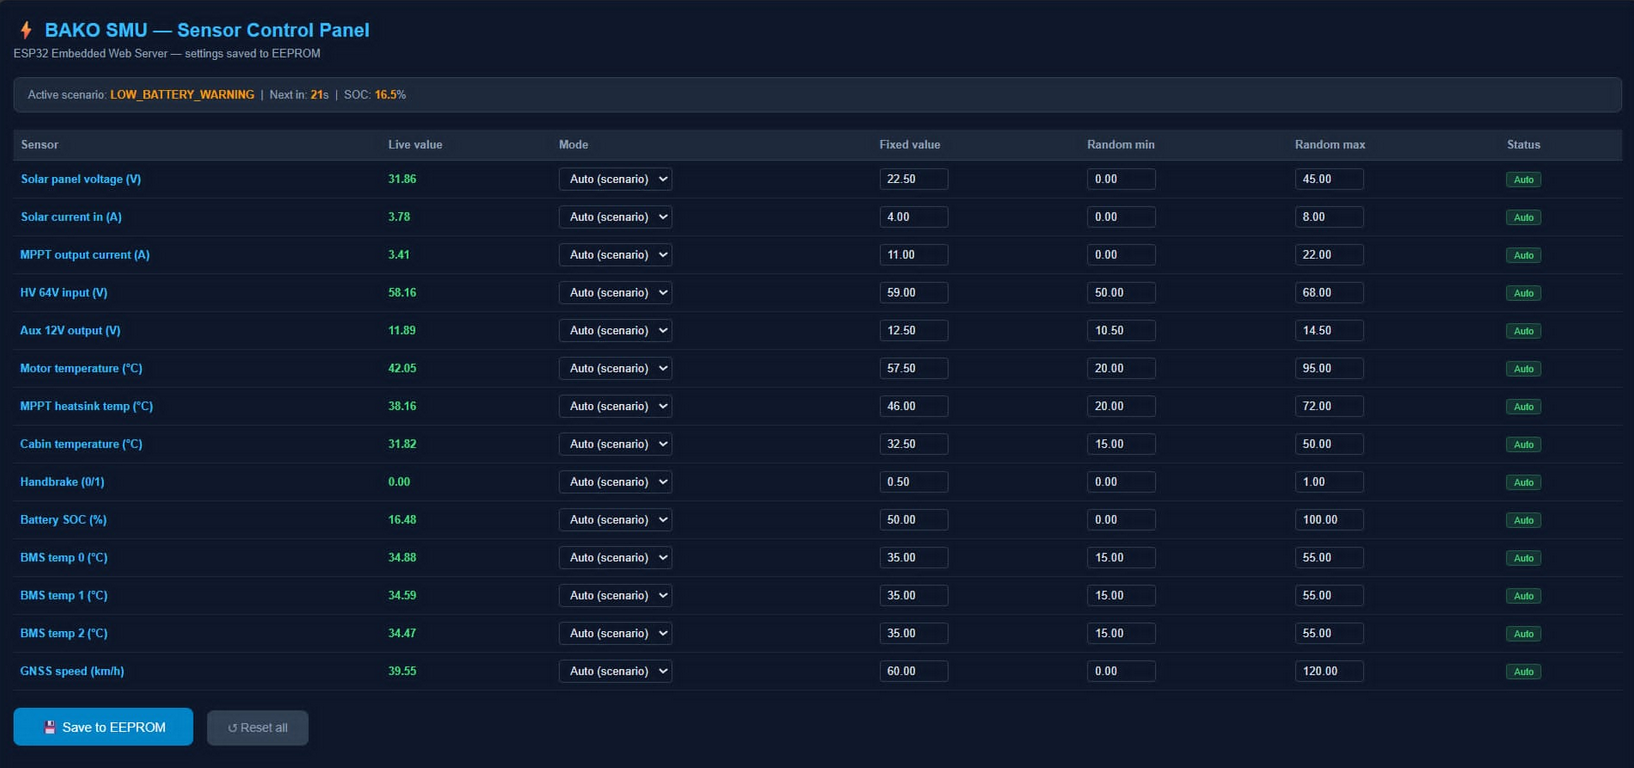
\includegraphics[width=\textwidth]{images/simulator-control-panel.png}
    \caption{BAKO SMU Sensor Control Panel --- browser-based interface served by the ESP32 firmware simulator, showing all 14 sensor channels with live values, scenario mode selectors, and manual override controls.}
    \label{fig:simulator-panel}
\end{figure}

To improve usability and persistence, all sensor configuration parameters are stored locally in \textbf{EEPROM}, allowing settings to remain available after reboot or power cycling. Furthermore, an offline telemetry buffering mechanism was implemented using the ESP32 \textbf{SPIFFS} internal flash filesystem. When the TCP connection becomes unavailable, telemetry data is temporarily stored locally and automatically retransmitted once connectivity is restored.

This testing environment significantly reduces dependency on the physical vehicle during development and debugging phases. It also provides a reproducible and controlled platform for validating embedded communication pipelines, dashboard integration, telemetry visualisation, offline recovery behaviour, and system operation under multiple simulated conditions.

\subsubsection*{Python Log Replay Tool}

The script \texttt{simulate.py} provides a complementary simulation path that uses a captured real-vehicle CAN log rather than synthetic data. It reads the log file \texttt{data/raw/bms\_log\_2026-03-10T10-20-02.txt} (containing 3197 frames from a real on-vehicle session) and pipes it into the live server over a virtual serial port, allowing the full dashboard to operate on authentic data without physical hardware.

The replay sequence is:
\begin{enumerate}
    \item A virtual PTY (pseudo-terminal) pair is created using \texttt{socat}. One end is handed to the server as its serial port; the other is used by the feeder thread to write log lines.
    \item The FastAPI server is launched as a subprocess on port 8787.
    \item Once the server's \texttt{/api/mode} endpoint responds, the script posts \texttt{mode=serial} with the virtual PTY path, switching the server into serial-reader mode.
    \item The browser is opened automatically at \texttt{http://localhost:8787}.
    \item Log frames are streamed to the PTY feeder end with inter-frame delays derived from the original timestamps, scaled by a configurable speed multiplier (default 2$\times$). The log loops continuously until interrupted.
\end{enumerate}

The \texttt{--speed} argument allows accelerated replay (e.g., \texttt{--speed 10} for rapid regression testing) while \texttt{--no-browser} suppresses the automatic browser launch for headless test environments.

\subsubsection{Python Emulator Extension: Local Storage and TCP Transmission}

As an extension to the Python-based sensor emulator, a local storage and TCP communication layer was implemented to improve telemetry reliability and prepare the emulator for remote server integration.

The emulator first generates realistic values for the 14 external sensors, including current, voltage, temperature, handbrake state, and GNSS data. Each generated record is then stored locally in a SQLite database before any transmission attempt. This ensures that telemetry data is preserved even if the network connection is unavailable.

A TCP socket client was also developed to transmit unsent records to a remote server. During local testing, a simulated TCP server was used to reproduce the behaviour of the future VPS server. When the server is available, the client sends the stored telemetry records and marks them as sent in the local database. If the connection fails, the data remains stored locally and is retried automatically during the next transmission cycle.

This architecture implements a \textbf{store-and-forward} mechanism. It allows the emulator to continue operating during internet outages while preventing telemetry loss. Once VPS access is provided, only the server IP address in the TCP client configuration needs to be replaced to enable remote deployment.

The implemented extension therefore adds three key capabilities to the emulator:
\begin{itemize}
    \item local persistence of generated telemetry data using SQLite;
    \item TCP socket transmission instead of WebSocket communication;
    \item offline buffering and automatic retransmission after reconnection.
\end{itemize}

This work prepares the emulator for reliable remote telemetry testing and aligns it with the cloud connectivity objectives of the BAKO monitoring system.

% ─────────────────────────────────────────────────────────────────────────────
\subsection{Wi-Fi Dashboard Connection}
\label{sec:wifi-dashboard}

The \textbf{Wi-Fi dashboard connection} mode allows the FastAPI server to receive telemetry data from the ESP32 over a TCP socket rather than a USB serial port. This mode was implemented to support wireless monitoring sessions where connecting a USB cable to the vehicle is impractical.

\subsubsection*{ReaderManager --- Runtime-Switchable Transport}

The \texttt{ReaderManager} class in \texttt{server\_frame\_parser\_Json.py} owns a single background reader thread and exposes three selectable transport modes:

\begin{description}
    \item[\texttt{serial}] Opens the specified USB/UART serial port (auto-detected or manually specified) and reads newline-delimited CAN frame text.
    \item[\texttt{wifi}] Opens a TCP client socket to the ESP32 AP at the configured IP and port, and reads the same frame format over Wi-Fi.
    \item[\texttt{off}] No reader running; the dashboard displays the ``Disconnected'' state.
\end{description}

Mode selection is persisted to \texttt{mode\_config.json} and restored automatically on the next server launch. When the operator switches mode via the dashboard UI (Section~\ref{fig:mode-selector}), \texttt{ReaderManager} signals the current reader thread to stop (via a \texttt{threading.Event}), waits up to 4~seconds for it to join, then starts the new reader thread with updated configuration.

\subsubsection*{Wi-Fi Reader Loop}

The \texttt{wifi\_reader\_loop()} function implements the TCP client. Its behaviour is:

\begin{enumerate}
    \item Open a \texttt{socket.SOCK\_STREAM} TCP connection to the ESP32 at the configured IP and port (default 192.168.4.1:9000) with a 4-second connection timeout.
    \item On successful connection, set \texttt{state["connected"] = True} and \texttt{state["mode"] = "wifi"} under the shared state lock.
    \item Read the socket in 4096-byte chunks with a 1-second timeout. Split on newline boundaries and pass each complete line to \texttt{process\_line()}, the same CAN-frame parser used in serial mode. A partial final line is buffered until the next chunk arrives.
    \item On any socket error or lost connection, set \texttt{state["connected"] = False}, log the error to \texttt{state["last\_error"]}, wait 2~seconds, and retry the TCP connection. This automatic reconnection handles the case where the ESP32 reboots or moves out of range.
    \item On stop signal, close the socket and exit.
\end{enumerate}

Because the frame format emitted by the ESP32 over Wi-Fi TCP is identical to that emitted over USB Serial, the parsing layer (\texttt{process\_line()}) requires no modification for Wi-Fi mode. The dashboard connection status indicator correctly reflects the Wi-Fi connection state in real time.

% ─────────────────────────────────────────────────────────────────────────────
\subsection{BLE Companion Interface}
\label{sec:ble}

Bluetooth Low Energy (BLE) connectivity was implemented to complement the Wi-Fi dashboard by providing a lightweight, phone-friendly monitoring channel for the vehicle operator. BLE was selected due to its low power consumption, wide smartphone compatibility, and sufficient data throughput for sensor-based telemetry. The ESP32 chip includes a built-in dual-mode Bluetooth radio supporting BLE 4.2 / 5.0, making BLE a zero-hardware-cost addition to the platform.

\subsubsection*{Hardware and Software Platform}

The BLE module runs entirely on the ESP32 development board using the \textbf{NimBLE-Arduino} library, a lightweight and memory-efficient BLE stack well-suited to embedded firmware. Testing was performed using Android BLE scanner applications, including nRF Connect, and a custom Android companion application.

\subsubsection*{GATT Architecture}

The communication follows a GATT (Generic Attribute Profile) client--server model. The ESP32 acts as the \textbf{GATT Server}, exposing a vehicle telemetry service; the Android application acts as the \textbf{GATT Client}, subscribing to and receiving characteristic notifications.

The telemetry service is identified by a project-specific 128-bit base UUID \texttt{12345678-0000-0000-0000-0000000000xx}. Six characteristics are defined, each carrying one real-time sensor stream:

\begin{table}[H]
\centering
\caption{BLE GATT Characteristic Map}
\label{tab:ble-characteristics}
\begin{tabular}{ll}
\toprule
\textbf{Parameter} & \textbf{Characteristic UUID} \\
\midrule
Speed       & \texttt{12345678-0000-0000-0000-000000000001} \\
Voltage     & \texttt{12345678-0000-0000-0000-000000000002} \\
SOC         & \texttt{12345678-0000-0000-0000-000000000003} \\
Current     & \texttt{12345678-0000-0000-0000-000000000004} \\
Temperature & \texttt{12345678-0000-0000-0000-000000000005} \\
RPM         & \texttt{12345678-0000-0000-0000-000000000006} \\
\bottomrule
\end{tabular}
\end{table}

\subsubsection*{ESP32 Implementation}

The BLE stack is initialised in \texttt{setup()} using the NimBLE API:

\begin{enumerate}
    \item \texttt{NimBLEDevice::init()} --- initialises BLE with the device name \textbf{BAKO-Dashboard}, which is broadcast in the advertising packet so that Android devices can discover the ESP32 by name.
    \item \texttt{createServer()} --- creates the GATT server and registers connection callbacks.
    \item \texttt{createService()} --- defines the vehicle telemetry service under its UUID.
    \item \texttt{createCharacteristic()} --- defines each of the six data channels with \texttt{READ | NOTIFY} properties.
    \item \texttt{startAdvertising()} --- makes the device continuously discoverable.
\end{enumerate}

Sensor values are updated every 500~ms in the main loop. Each value is converted to a string and pushed via \texttt{notify()}, which delivers it to any subscribed Android client in real time. Notifications are only sent when a client is connected, avoiding unnecessary radio activity.

\subsubsection*{Connection Handling}

A callback class overrides two methods to manage the BLE connection lifecycle:

\begin{itemize}
    \item \textbf{onConnect} --- triggered when an Android device establishes a connection; suspends advertising to dedicate bandwidth to the active client.
    \item \textbf{onDisconnect} --- automatically restarts advertising so the ESP32 remains discoverable after the client disconnects or moves out of range.
\end{itemize}

This ensures continuous availability without manual reset.

\subsubsection*{Android Integration}

The Android companion application scans for BLE devices by advertised name. After connecting to \textbf{BAKO-Dashboard}:

\begin{enumerate}
    \item The app discovers the GATT telemetry service.
    \item It subscribes to all six characteristics and enables notifications.
    \item Live values (speed, SOC, voltage, current, temperature, RPM) are displayed on a real-time dashboard interface.
\end{enumerate}

\subsubsection*{Coexistence with Wi-Fi}

The ESP32 shares its radio between Wi-Fi and BLE using time-division multiplexing managed by the ESP-IDF coexistence driver. Enabling BLE advertising alongside the Wi-Fi AP increases the Wi-Fi beacon interval slightly but does not affect the cloud GPRS data stream, which runs over the SIM800L UART and is entirely independent of the radio.

\subsubsection*{Challenges Encountered}

\paragraph{Device visibility on Android.}
Initially the ESP32 BLE device did not appear consistently in BLE scanning applications. Investigation revealed that the advertising packet was missing a complete scan response entry for the device name. The issue was resolved by explicitly configuring the NimBLE advertising parameters to include the device name in both the advertising data and the scan response packet, and by ensuring that \texttt{startAdvertising()} is called only after the GATT service is fully initialised.

\paragraph{Apple iOS compatibility.}
Testing on iOS devices proved more restrictive. iOS enforces stricter BLE scanning rules than Android: devices may not appear unless they advertise complete service UUIDs, background scanning is limited, and some characteristics require explicit bonding before they become visible to the application layer. As a result, Android was adopted as the primary testing and deployment platform, where tools such as nRF Connect provide detailed GATT inspection and ease of debugging. iOS support is deferred to a future firmware and app revision.


\clearpage

\section{Cloud Connectivity \& IoT}

\subsection{End-to-End Pipeline Sequence}

Figure~\ref{fig:diag-sequence} shows the complete message sequence for a single 5-second publish cycle, from CAN frame reception on the ESP32 through to dashboard rendering in the browser.

\begin{figure}[H]
    \centering
    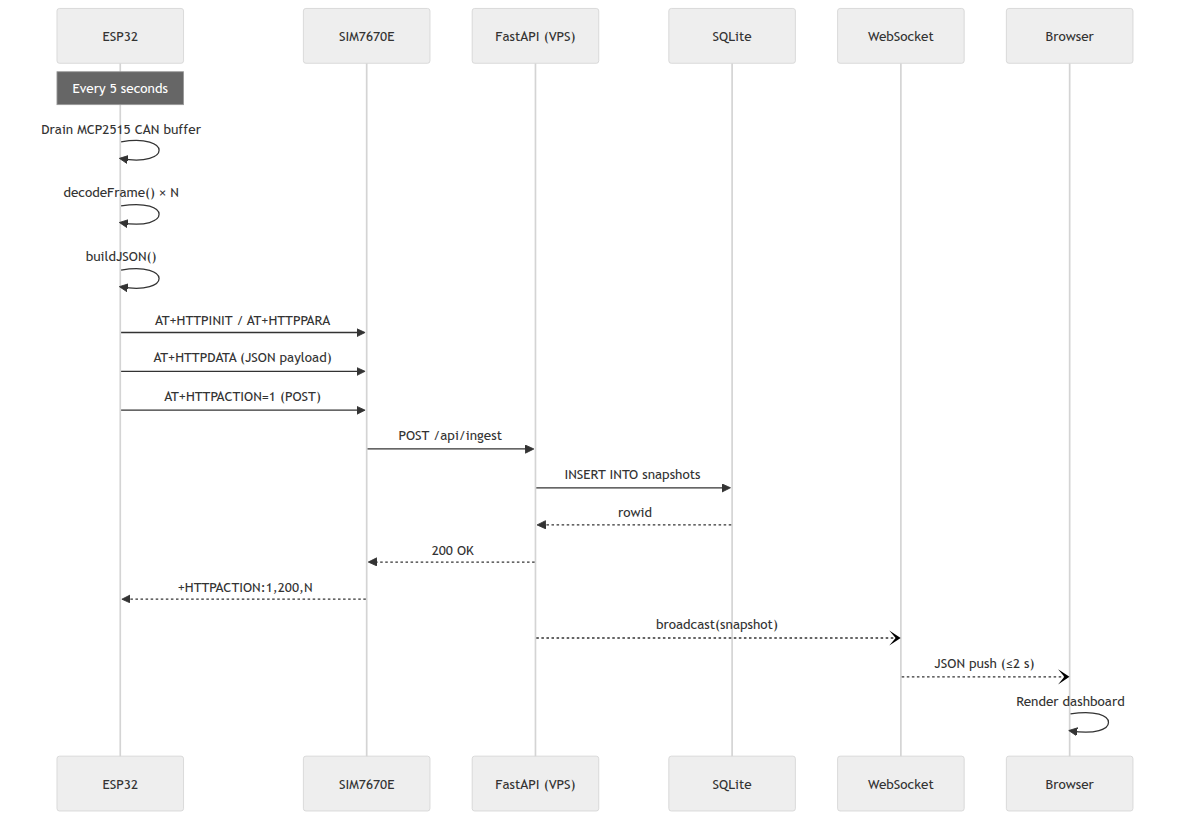
\includegraphics[width=\textwidth]{images/diag-sequence.png}
    \caption{End-to-end cloud telemetry sequence diagram: ESP32 CAN drain and JSON build, SIM800L AT command exchange, FastAPI ingest and SQLite write, WebSocket broadcast, and browser render --- one complete cycle every 5 seconds.}\label{fig:diag-sequence}
\end{figure}

This section describes the complete cloud telemetry pipeline designed and implemented for the Bako OBD ISS platform~\cite{evmonitoring}. The pipeline carries live battery data from the vehicle's CAN bus to a remote web dashboard through a sequence of embedded, network, server, and browser components. The architecture was designed to be hardware-independent: the same dashboard and backend serve both a direct USB serial connection (for lab use) and a cellular GPRS connection from the field.

% ─────────────────────────────────────────────────────────────────────────────
\subsection{Telematics \& Data Acquisition}

Telematics in this project refers to the capture, local decoding, and wireless transmission of battery state data from the moving vehicle to a remote server.

\subsubsection{On-Vehicle Data Acquisition}

Data acquisition begins at the O'CELL IFS60.8-500-F-E3 BMS, which continuously transmits CAN frames on a 250 kbps SAE J1939 bus. The ESP32 microcontroller, equipped with an MCP2515 CAN transceiver, receives all frames on this bus and decodes them in real time using the firmware described in Section~\ref{sec:bms-firmware}.

The BMS transmits at two rates. High-priority operational frames (0x18FF28F4 and 0x18FE28F4) arrive every 100 ms and carry pack voltage, current, SOC, and fault status. Lower-priority frames carrying cell-level voltages and temperatures arrive every 500 ms. At 250 kbps the bus is far from saturated; the five BMS frame types together occupy less than 2\% of available bandwidth.

\subsubsection{Snapshot Aggregation and Publish Cadence}

Because the HTTP transaction over the cellular module takes up to 5 seconds (bearer setup, DNS, TCP handshake, data transfer), it is not feasible to transmit every individual CAN frame to the cloud. Instead, the firmware implements a \textbf{snapshot model}: all incoming frames are decoded and merged into a single \texttt{BMSData} struct that always holds the most recent value for each field. Every 5 seconds, this struct is serialized into a single JSON document and sent as one HTTP POST to the VPS.

This approach has several advantages:
\begin{itemize}
    \item The cloud endpoint receives at most 12 snapshots per minute regardless of CAN bus activity.
    \item Each snapshot is self-contained and requires no state from previous snapshots to be interpreted.
    \item CAN frames continue to be decoded during the HTTP transaction, so the struct is fully populated before the next publish cycle.
\end{itemize}

\subsubsection{Cellular Connectivity — SIM800L GPRS}

Wireless transmission is handled by a \textbf{SIM800L GSM/GPRS module} connected to the ESP32 via HardwareSerial UART1. The module establishes a GPRS bearer using the carrier's APN, then uses the AT+HTTP* command set to perform a standard HTTP POST to the VPS endpoint.

The connection lifecycle at startup is:
\begin{enumerate}
    \item \texttt{AT+CPIN?} — verify SIM card is ready (retried up to 6 times after a reboot).
    \item \texttt{AT+CSQ} — check signal quality.
    \item \texttt{AT+CREG?} — confirm network registration.
    \item \texttt{AT+SAPBR=3,1,...} — configure bearer (APN, username, password).
    \item \texttt{AT+SAPBR=1,1} — open the GPRS bearer (up to 25 s).
    \item \texttt{AT+SAPBR=2,1} — confirm the bearer is active and has an IP address.
\end{enumerate}

If the bearer fails to open, the ESP32 retries the full sequence up to three times before invoking a soft restart (\texttt{ESP.restart()}).

\subsubsection{Network Timestamp}

To provide accurate event timestamps regardless of the vehicle's location, the firmware reads the network time from the SIM card using \texttt{AT+CCLK?} before each publish cycle. The returned timestamp (format \texttt{yy/MM/dd,HH:mm:ss\textpm zz}) is included in the JSON payload as the \texttt{timestamp} field. If the modem does not return a valid timestamp (e.g., during initial bearer setup), the firmware falls back to \texttt{uptime\_ms} from \texttt{millis()}.

% ─────────────────────────────────────────────────────────────────────────────
\subsection{Cloud Platform Configuration}

\subsubsection{Platform Choice}

The cloud backend runs on a \textbf{Virtual Private Server (VPS)} — a Linux instance with a public IP address — rather than a managed cloud database service. This design decision was made for the following reasons:

\begin{itemize}
    \item \textbf{No third-party dependency}: the entire data path (ingest $\rightarrow$ storage $\rightarrow$ streaming) is contained within a single process under direct control of the project team.
    \item \textbf{Simplicity}: the SIM800L communicates over plain HTTP, eliminating the need for TLS certificate handling on the embedded side.
    \item \textbf{Cost}: a VPS is significantly cheaper than a managed real-time database for low-throughput IoT workloads.
    \item \textbf{Full observability}: the server log, database file, and WebSocket connections are all directly inspectable via SSH.
\end{itemize}

\subsubsection{Backend Runtime}

The backend is a single Python file (\texttt{backend/server.py}) running under \textbf{Uvicorn}~\cite{uvicorn}, an ASGI server. The application framework is \textbf{FastAPI}~\cite{fastapi}, which provides automatic OpenAPI documentation, WebSocket support~\cite{rfc6455}, and asynchronous request handling. The dependencies are minimal by design:

\begin{table}[h]
    \centering
    \caption{Backend Python Dependencies}
    \label{tab:backend-deps}
    \begin{tabular}{llp{7cm}}
        \toprule
        \textbf{Package} & \textbf{Version} & \textbf{Purpose} \\
        \midrule
        \texttt{fastapi}  & 0.115.0 & Web framework, WebSocket, routing \\
        \texttt{uvicorn}  & 0.29.0  & ASGI server (serves HTTP and WebSocket on one port) \\
        \texttt{pyserial} & 3.5     & Serial port I/O for USB/SERIAL mode \\
        \bottomrule
    \end{tabular}
\end{table}

No external database client, message broker, or cloud SDK is required. The entire stack is started with a single command:

\begin{verbatim}
python server.py --cloud-only
\end{verbatim}

The \texttt{--cloud-only} flag suppresses serial port detection so the server starts cleanly on a headless VPS without a USB device attached.

\subsubsection{Environment Variables}

Server behavior is controlled by three environment variables, summarized in Table~\ref{tab:env-vars}:

\begin{table}[h]
    \centering
    \caption{Server Environment Variables}
    \label{tab:env-vars}
    \begin{tabular}{lll}
        \toprule
        \textbf{Variable} & \textbf{Default} & \textbf{Purpose} \\
        \midrule
        \texttt{BMS\_API\_KEY} & \texttt{bako-bms-2024} & Shared secret for \texttt{POST /api/ingest} authentication \\
        \texttt{HOST}          & \texttt{0.0.0.0}       & Bind address (all interfaces on VPS) \\
        \texttt{PORT}          & \texttt{8787}          & TCP port for HTTP and WebSocket traffic \\
        \bottomrule
    \end{tabular}
\end{table}

% ─────────────────────────────────────────────────────────────────────────────
\subsection{Data Pipeline \& Storage}

\subsubsection{Pipeline Overview}

The end-to-end data pipeline operates as follows and is illustrated in Figure~\ref{fig:cloud-pipeline}:

\begin{enumerate}
    \item The ESP32 reads CAN frames and decodes them into a \texttt{BMSData} struct (on-vehicle).
    \item Every 5 seconds, the struct is serialized into a JSON document and sent as \texttt{POST /api/ingest} to the VPS, with an \texttt{X-Api-Key} header for authentication.
    \item The server validates the API key, stores the payload in SQLite, and updates the in-memory \texttt{\_cloud\_state} dictionary.
    \item Browser clients connected to \texttt{/ws/cloud} receive the latest \texttt{\_cloud\_state} every 2 seconds via WebSocket push.
\end{enumerate}

\begin{figure}[p]
    \centering
    \rotatebox{90}{%
        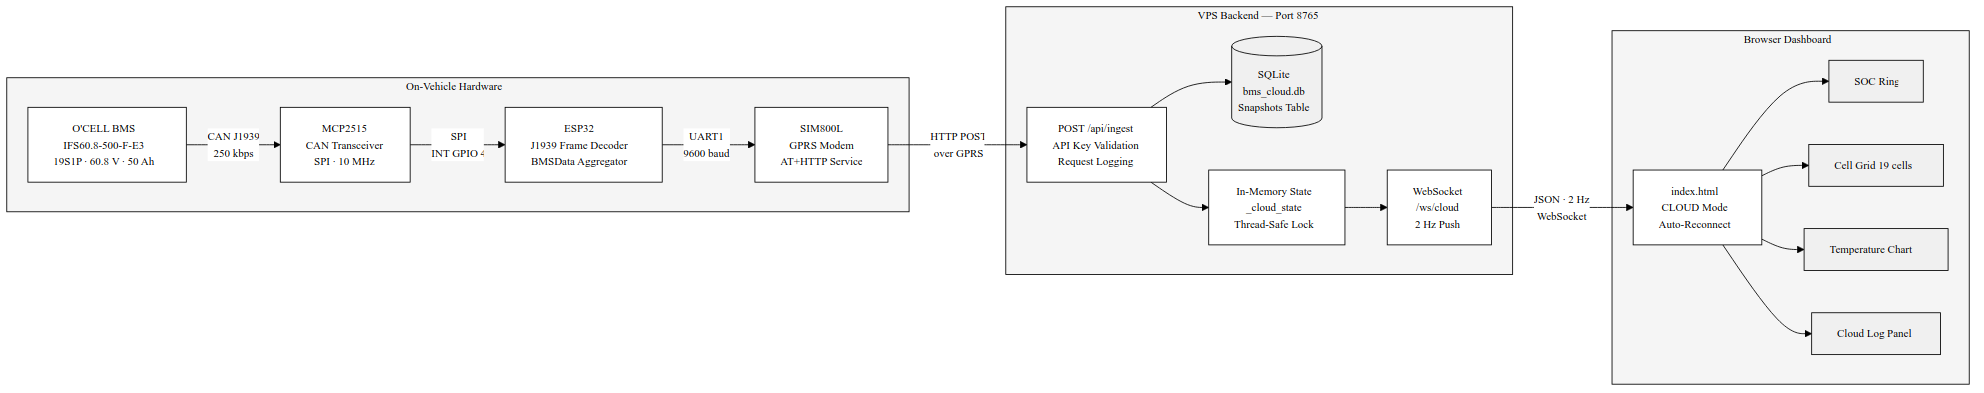
\includegraphics[width=0.92\textheight]{images/cloud-pipeline.png}%
    }
    \caption{Complete data pipeline from CAN bus to browser}
    \label{fig:cloud-pipeline}
\end{figure}

\subsubsection{Ingest Endpoint}

The \texttt{POST /api/ingest} endpoint is the sole entry point for ESP32 data. Its implementation:

\begin{enumerate}
    \item Validates the \texttt{X-Api-Key} header against the \texttt{BMS\_API\_KEY} environment variable. An incorrect key returns HTTP 401.
    \item Extracts the timestamp, device ID, cell count, SOC, and pack voltage from the JSON body for logging.
    \item Runs a non-blocking SQLite insert via \texttt{asyncio.run\_in\_executor()} to avoid blocking the event loop during disk I/O.
    \item Updates the in-memory \texttt{\_cloud\_state} dict atomically under a threading lock (because the serial reader thread and the asyncio event loop share this state).
    \item Appends a timestamped \texttt{[RECV]} entry to the cloud communication log.
    \item Returns \texttt{\{"status": "ok", "ts": ...\}} with HTTP 200.
\end{enumerate}

\subsubsection{SQLite Persistent Storage}

Received snapshots are persisted in a local SQLite database (\texttt{backend/bms\_cloud.db}) for historical analysis and post-session review. The schema is intentionally minimal:

\begin{verbatim}
CREATE TABLE IF NOT EXISTS snapshots (
    id        INTEGER PRIMARY KEY AUTOINCREMENT,
    ts        TEXT    NOT NULL,
    device_id TEXT    NOT NULL DEFAULT 'esp32',
    payload   TEXT    NOT NULL
);
\end{verbatim}

The full JSON payload is stored as a text column, which avoids schema migrations when new fields are added to the firmware. Queries for the \texttt{/api/history} endpoint retrieve records ordered by descending \texttt{id} (newest first) with a configurable limit. SQLite was chosen over a full database server because:

\begin{itemize}
    \item At one snapshot per 5 seconds, a full day of operation produces only $\sim$17,000 rows ($\sim$10 MB), well within SQLite's performance envelope.
    \item No separate database process or network socket is required.
    \item The database file can be copied directly from the VPS for offline analysis with standard tools.
\end{itemize}

A similar storage mechanism was also implemented on the Python emulator side, where generated telemetry records are stored locally in SQLite before being transmitted through a TCP socket client.

\subsubsection{In-Memory State and WebSocket Push}

In addition to SQLite, the server maintains an in-memory dictionary (\texttt{\_cloud\_state}) that always holds the most recently received snapshot. This allows the \texttt{/ws/cloud} WebSocket handler to serve browser clients at 2 Hz with zero disk I/O per push.

The in-memory state is initialized to \texttt{\{"connected": false, "source": "cloud"\}} on startup. The dashboard interprets \texttt{connected: false} as a "waiting for ESP32" state and displays a yellow indicator to the user rather than an error.

% ─────────────────────────────────────────────────────────────────────────────
\subsection{Remote Monitoring Dashboard}

\subsubsection{Architecture}

The dashboard is a \textbf{single-page web application} served as a static HTML file (\texttt{frontend/index.html}) directly by the FastAPI backend via \texttt{GET /}. No separate web server, build tool, or JavaScript framework is required. All rendering logic is contained in vanilla JavaScript.

The dashboard connects to the backend over \textbf{WebSocket}, which provides a persistent, low-latency bidirectional channel. In SERIAL mode the WebSocket endpoint is \texttt{/ws} (10 Hz push from the serial reader); in CLOUD mode it is \texttt{/ws/cloud} (2 Hz push from the in-memory state). The user switches between modes using a toggle button in the header.

\subsubsection{Dashboard Panels}

Table~\ref{tab:cloud-dashboard-panels} summarizes the information panels displayed by the dashboard.

\begin{table}[h]
    \centering
    \caption{Dashboard Panel Summary}
    \label{tab:cloud-dashboard-panels}
    \begin{tabular}{lp{9cm}}
        \toprule
        \textbf{Panel} & \textbf{Contents} \\
        \midrule
        SOC ring        & Animated circular gauge showing voltage-derived SOC (\texttt{battery.soc}). BMS coulomb-counter SOC (\texttt{battery.soc\_bms}) is displayed below. \\
        Pack KPIs       & Pack voltage, current, discharge limit, charge request, and cell count in a card grid. \\
        Cell grid       & All 19 cells — individual voltage bars color-coded by threshold (overvoltage / full / good / normal / low / undervoltage), with min/max/avg/spread statistics. \\
        Temperature     & Up to 4 temperature probe readings with color-coded bars and a rolling time-series chart. \\
        Serial monitor  & Raw CAN frame log with text export and Excel export capabilities. \\
        Cloud log       & Real-time cloud communication events (RECV / WS / ERR), polled from \texttt{/api/cloud-log} every 2 seconds, independent of the SERIAL/CLOUD source toggle. \\
        \bottomrule
    \end{tabular}
\end{table}

\subsubsection{Connection Status Indicator}

The dashboard header contains a three-state connection indicator that provides immediate visual feedback:

\begin{description}
    \item[\textcolor{green}{Green — Live}] WebSocket is open and the last received message contained \texttt{connected: true}.
    \item[\textcolor{yellow}{Yellow — Waiting}] WebSocket is open but \texttt{connected: false} (backend is running but no ESP32 data has arrived yet).
    \item[\textcolor{red}{Red — Disconnected}] WebSocket is closed or encountered a network error.
\end{description}

\subsubsection{Auto-Reconnect}

If the WebSocket closes unexpectedly (server restart, network interruption), the browser automatically attempts to reconnect every 5 seconds. The overlay is re-displayed during the disconnected interval. This behavior is handled entirely client-side and requires no intervention from the user.

% ─────────────────────────────────────────────────────────────────────────────
\subsection{Security \& Cybersecurity}

\subsubsection{API Key Authentication}

The \texttt{POST /api/ingest} endpoint is protected by a shared secret transmitted as the \texttt{X-Api-Key} HTTP header. The server compares the received key against the \texttt{BMS\_API\_KEY} environment variable. Requests with a missing or incorrect key are rejected with HTTP 401 before any data is read from the body, and an \texttt{[ERR]} entry is appended to the cloud log.

The API key is configured separately on the firmware (\texttt{VPS\_API\_KEY} in \texttt{include/secrets.h}, which is in \texttt{.gitignore}) and on the server (environment variable), so the secret is never committed to the repository.

\subsubsection{Transport Layer}

Communication between the SIM800L and the VPS uses plain HTTP. While this means the payload is not encrypted in transit, the following mitigating factors apply to this deployment context:

\begin{itemize}
    \item The data transmitted is battery telemetry (voltages, temperatures, SOC) — not personally identifiable information or control commands.
    \item The VPS port is firewalled to accept connections only on the designated port.
    \item The API key protects against unauthorized data injection.
\end{itemize}

For a production deployment, upgrading to HTTPS requires enabling TLS on the SIM800L (\texttt{AT+HTTPSSL=1}) and deploying a self-signed or CA-signed certificate, or using an Nginx reverse proxy with Let's Encrypt on the VPS side.

\subsubsection{WebSocket and Dashboard Access}

The dashboard itself is served over plain HTTP and the WebSocket connection is unencrypted. Since the dashboard is intended for use on a private network or VPN-protected VPS, this is considered acceptable for the current project scope. Adding HTTPS would require an SSL certificate (e.g., from Let's Encrypt) and an Nginx reverse proxy, which is a straightforward extension if needed.

% ─────────────────────────────────────────────────────────────────────────────
\subsection{API Documentation}

The FastAPI backend exposes the following endpoints, summarized in Table~\ref{tab:api-endpoints}. FastAPI generates interactive Swagger UI documentation automatically at \texttt{/docs} when the server is running.

\begin{table}[h]
    \centering
    \caption{Backend API Endpoint Reference}
    \label{tab:api-endpoints}
    \begin{tabular}{llp{7.5cm}}
        \toprule
        \textbf{Method} & \textbf{Path} & \textbf{Description} \\
        \midrule
        GET  & \texttt{/}                        & Serves the dashboard HTML file. \\
        WS   & \texttt{/ws}                      & Serial stream — pushes BMS JSON to the browser at 10 Hz. Active when an ESP32 is connected via USB. \\
        WS   & \texttt{/ws/cloud}                & Cloud stream — pushes the latest in-memory snapshot at 2 Hz. \\
        POST & \texttt{/api/ingest}              & Receives a BMS JSON snapshot from the ESP32. Requires header \texttt{X-Api-Key}. Returns \texttt{\{status: ok, ts: ...\}}. \\
        GET  & \texttt{/api/latest}              & Returns the most recent snapshot as JSON. \\
        GET  & \texttt{/api/history?limit=N}     & Returns the last $N$ snapshots from SQLite, newest first (default $N$ = 100, max 1000). \\
        GET  & \texttt{/api/cloud-log}           & Returns the last 100 cloud communication events as a JSON array of timestamped strings. \\
        \bottomrule
    \end{tabular}
\end{table}

\subsubsection{Ingest Payload Schema}

The JSON body sent by the ESP32 to \texttt{POST /api/ingest} uses a \textbf{nested object structure} organized into five top-level sections. This design allows each subsystem (battery, thermal, solar, DC/DC, vehicle) to be extended independently without changing the ingest endpoint. Table~\ref{tab:json-schema-top} describes the top-level envelope, and Table~\ref{tab:json-schema-battery} expands the \texttt{battery} object.

\begin{table}[h]
    \centering
    \caption{ESP32 JSON Payload — Top-Level Envelope}
    \label{tab:json-schema-top}
    \begin{tabular}{lll}
        \toprule
        \textbf{Field} & \textbf{Type} & \textbf{Description} \\
        \midrule
        \texttt{device\_id}   & string & Configurable in \texttt{secrets.h} \\
        \texttt{timestamp}    & string & Network time from \texttt{AT+CCLK?} (or \texttt{uptime\_ms} fallback) \\
        \texttt{source}       & string & Always \texttt{"esp32-SIM800L"} \\
        \texttt{connected}    & bool   & Always \texttt{true} when sent by the ESP32 \\
        \texttt{frame\_count} & int    & Cumulative CAN frames decoded since boot \\
        \texttt{fault\_level} & int    & 0 = normal, 1 = serious fault \\
        \texttt{error\_code}  & int    & BMS fault code (see Table~\ref{tab:fault-codes}) \\
        \texttt{battery}      & object & Battery pack data — see Table~\ref{tab:json-schema-battery} \\
        \texttt{temperatures} & object & Thermal data from all probes \\
        \texttt{solar}        & object & Solar MPPT data (pre/post converter) \\
        \texttt{dc\_dc}       & object & DC/DC converter outputs (64 V and 12 V rails) \\
        \texttt{vehicle}      & object & Vehicle-level status (handbrake, etc.) \\
        \bottomrule
    \end{tabular}
\end{table}

\begin{table}[h]
    \centering
    \caption{ESP32 JSON Payload — \texttt{battery} Object Fields}
    \label{tab:json-schema-battery}
    \begin{tabular}{lll}
        \toprule
        \textbf{Field} & \textbf{Type} & \textbf{Description} \\
        \midrule
        \texttt{pack\_v}          & float  & Pack voltage [V], 0.1 V resolution \\
        \texttt{pack\_current\_a} & float  & Pack current [A], + = discharge, $-$ = charge \\
        \texttt{soc}              & float  & Voltage-derived SOC [\%] \\
        \texttt{soc\_bms}         & int    & BMS coulomb-counter SOC [\%] \\
        \texttt{max\_disch\_a}    & float  & Maximum discharge current limit [A] \\
        \texttt{cell\_count}      & int    & Number of active cells decoded \\
        \texttt{cell\_avg\_mv}    & int    & Average cell voltage [mV] \\
        \texttt{cell\_min\_mv}    & int    & Minimum cell voltage [mV] \\
        \texttt{cell\_max\_mv}    & int    & Maximum cell voltage [mV] \\
        \texttt{cell\_spread\_mv} & int    & Max $-$ min cell voltage [mV] \\
        \texttt{cells}            & array  & 1-based array of \texttt{\{"mv", "status"\}} objects; index 0 = \texttt{null} \\
        \texttt{charger}          & object & \texttt{max\_charge\_v}, \texttt{max\_charge\_a}, \texttt{start\_signal} \\
        \texttt{status}           & object & Bit-field flags: charging, discharging, ready, contactors \\
        \bottomrule
    \end{tabular}
\end{table}

The \texttt{temperatures} object contains \texttt{battery\_avg\_c}, \texttt{battery\_min\_c}, \texttt{battery\_max\_c}, and a 1-based \texttt{battery\_cells} array (index 0 = \texttt{null}, indices 1--4 = probe readings in \textdegree C). Fields for sensors not yet instrumented (\texttt{motor\_c}, \texttt{mppt\_c}, \texttt{cabin\_c}) are present with value \texttt{null}, enabling the dashboard to display placeholders without schema changes when those sensors are added. The same pattern applies to \texttt{solar} and \texttt{dc\_dc} sub-objects.

\subsubsection{Example API Interaction}

The following \texttt{curl} command simulates an ESP32 posting a snapshot to the server during testing. On a successful ingest the server returns a timestamped acknowledgement and pushes the payload to any browser connected to \texttt{/ws/cloud} within 2 seconds.

\begin{verbatim}
curl -X POST http://YOUR_VPS_IP:8787/api/ingest \
  -H "Content-Type: application/json"           \
  -H "X-Api-Key: bako-bms-2024"                \
  -d '{
    "device_id": "esp32-bms-001",
    "connected": true,
    "fault_level": 0,
    "battery": {
      "soc": 87.4, "pack_v": 62.3,
      "cell_count": 19,
      "cells": [null, {"mv": 3280, "status": "good"}]
    },
    "temperatures": { "battery_avg_c": 21.0,
                      "battery_cells": [null, 21.0, 22.0, null, null] }
  }'
\end{verbatim}

\noindent The server responds with \texttt{\{"status": "ok", "ts": "2026-04-18T09:32:11.123456"\}}.

\clearpage

% Integration phase removed per project revision
\section{Implementation Phase}
\label{sec:implementation-phase}

\subsection{Prototype Build \& Bring-Up}

\subsubsection*{Vehicle Installation Context}

The ISS board is installed inside the BAKO Motors electric vehicle chassis beneath the driver seat, directly adjacent to the MPPT controller. This position gives the board short cable runs to the battery CAN bus connector, the MPPT current/voltage sense lines, and the vehicle 12~V supply rail, while keeping it sheGPRSred from direct exposure to rain and road debris. Figure~\ref{fig:bako-placement} shows the installation location on the vehicle frame.

\begin{figure}[H]
    \centering
    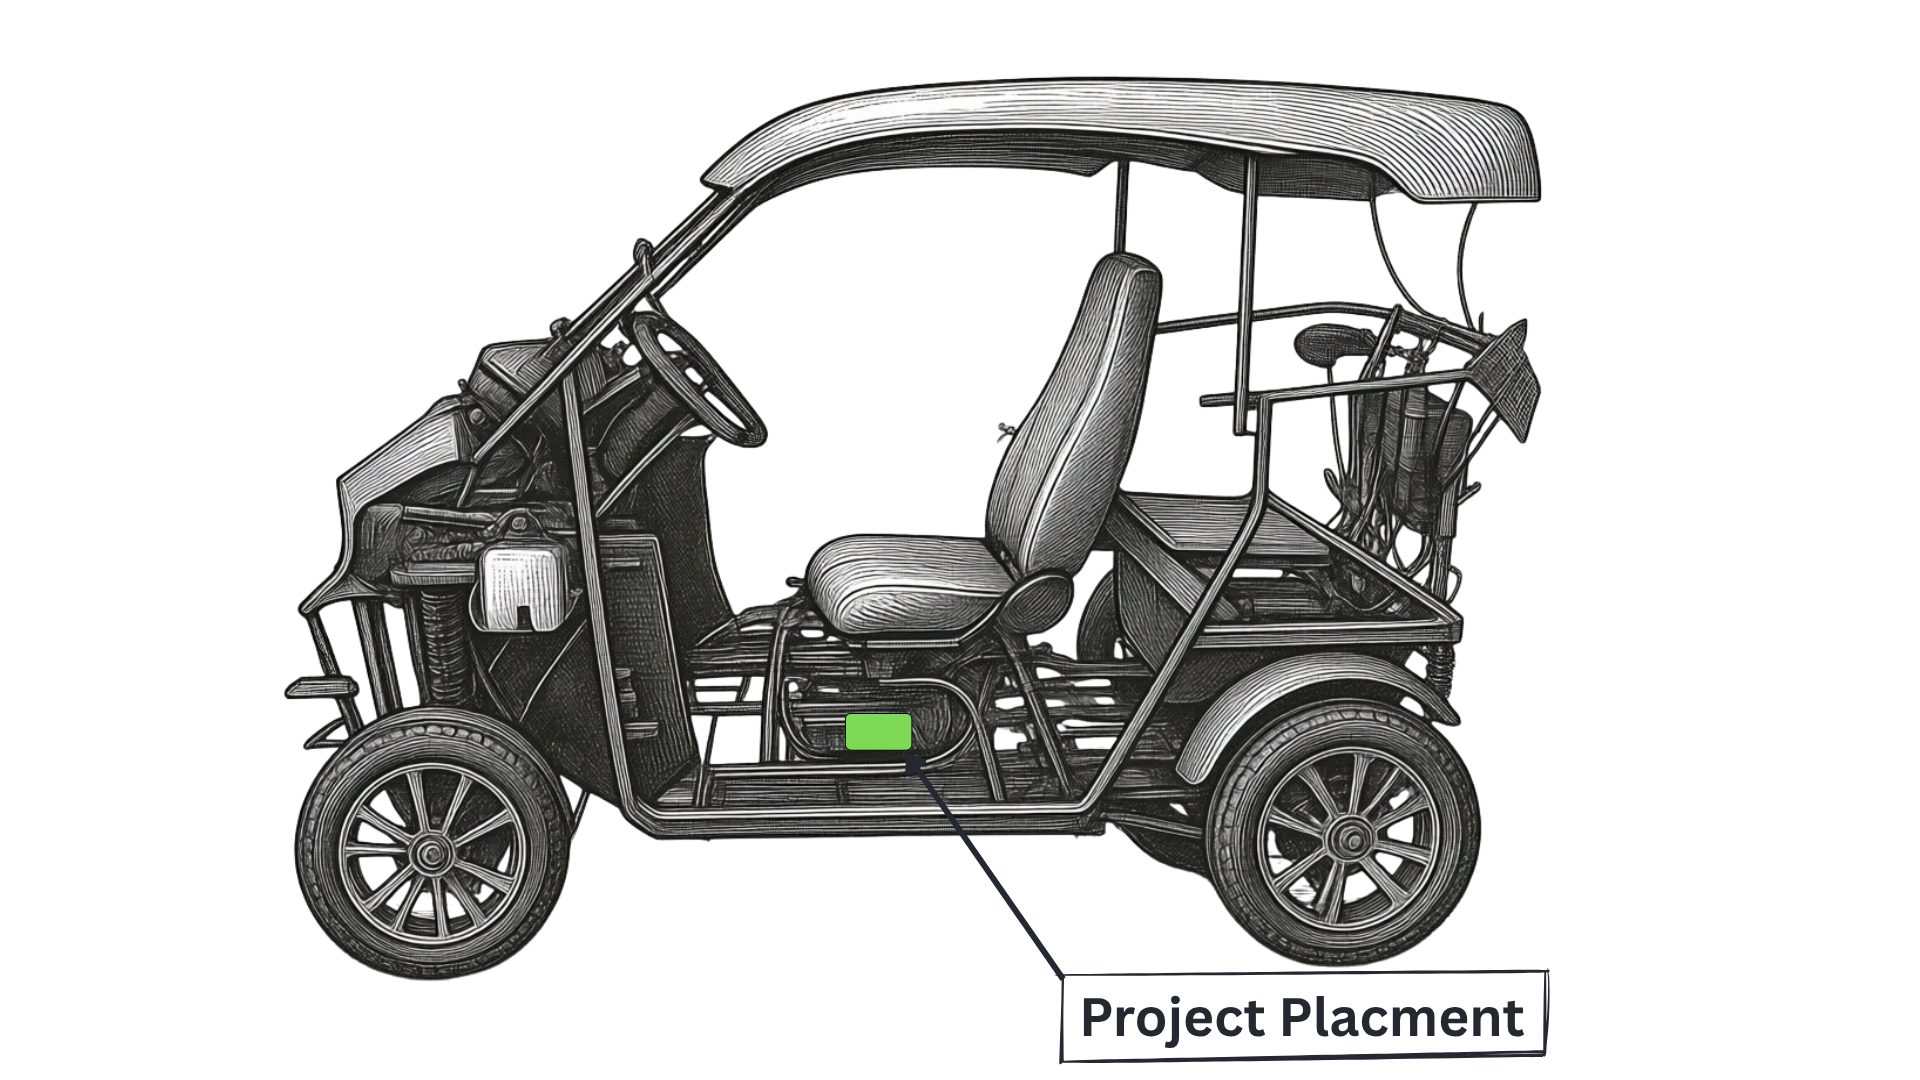
\includegraphics[width=\textwidth]{images/bako-placement.png}
    \caption{BAKO Motors vehicle with the ISS board installation location highlighted (green) --- mounted beneath the driver seat adjacent to the MPPT controller, with short harness runs to the CAN bus, power rail, and sensor connectors.}\label{fig:bako-placement}
\end{figure}

\subsubsection*{Bring-Up Sequence}

The custom PCB was populated and brought up using a structured nine-step sequence designed to isolate each subsystem before applying power to the full board. This approach minimised the risk of damage from wiring errors and made fault localisation straightforward.

\begin{enumerate}
    \item \textbf{Power-only verification.} The 12~V supply was connected with only the LM2596S-ADJ and the AMS1117 and LM7805 linear regulators populated. All three output rails (12~V, 5~V, 3.3~V) were measured and confirmed within $\pm 2\%$ of their target values before any other component was installed.

    \item \textbf{ESP32 base bring-up.} The ESP32-DEVKITC module was inserted and a minimal ``blink'' firmware flashed over USB. Successful LED blink confirmed that the 3.3~V rail was stable and that the module was programmable via PlatformIO. The OTA web portal (Section~\ref{sec:ota}) was also flashed at this stage to enable wireless reflashing for all subsequent development.

    \item \textbf{MCP2515 SPI communication.} One MCP2515 SPI module header (J17) was populated and a loopback test was run. The MCP2515 read-back of its control registers confirmed SPI integrity. A second module (J18) was then added and addressed independently via its dedicated chip-select line.

    \item \textbf{CAN bus receive test.} The TJA1051T transceiver was connected and the CAN connector J1 was wired to the O'CELL BMS. The ESP32 firmware was configured to listen passively (no ACK). Frame reception was confirmed by observing decoded 0x18FF28F4 pack-voltage frames on the serial monitor within 2~s of power-up.

    \item \textbf{DS18B20 1-Wire bring-up.} All three DS18B20 connectors (J6, J7, J8) were populated with sensors and the 4.7~k$\Omega$ pull-up verified. The firmware enumerated all three ROM addresses and began temperature polling at 1~s intervals. Readings were compared against a reference thermometer.

    \item \textbf{ACS712 current sensor calibration.} The two current sensor headers (J11, J16) were connected to the ACS712 modules. With zero current flowing, the ADC mid-point offset was measured and stored as a calibration constant. A known 5~A load was applied and the output compared against a reference clamp meter.

    \item \textbf{Voltage divider scaling verification.} The MPPT voltage input (J2) was driven from a bench power supply at three known voltages. The ESP32 ADC readings were compared against the calculated divider ratio and the calibration coefficient adjusted to eliminate the systematic offset.

    \item \textbf{SIM800L AT command verification.} The SIM800L module was powered on and AT commands were sent from the ESP32 over UART. SIM card detection, network registration, and GPRS bearer open were confirmed in sequence. An HTTP POST to the test endpoint was executed and the server acknowledged receipt.

    \item \textbf{Full integration smoke test.} All subsystems were enabled simultaneously. The firmware ran the cooperative main loop for 30~minutes with all sensors active. No watchdog triggers, stack overflows, or heap exhaustion events were observed. All sensor values appeared correctly on the WebSocket dashboard.
\end{enumerate}

Figure~\ref{fig:pcb-assembled} shows the physical outcome of the build: the bare PCB as received from the fabrication house (right) and the fully populated board after component soldering and module fitment (left). The assembled board carries the ESP32-DEVKITC, SIM800L GPRS cellular module, screw-terminal sensor connectors, and all passive components as specified in the BOM (Section~\ref{sec:components-inventory}).

\begin{figure}[H]
    \centering
    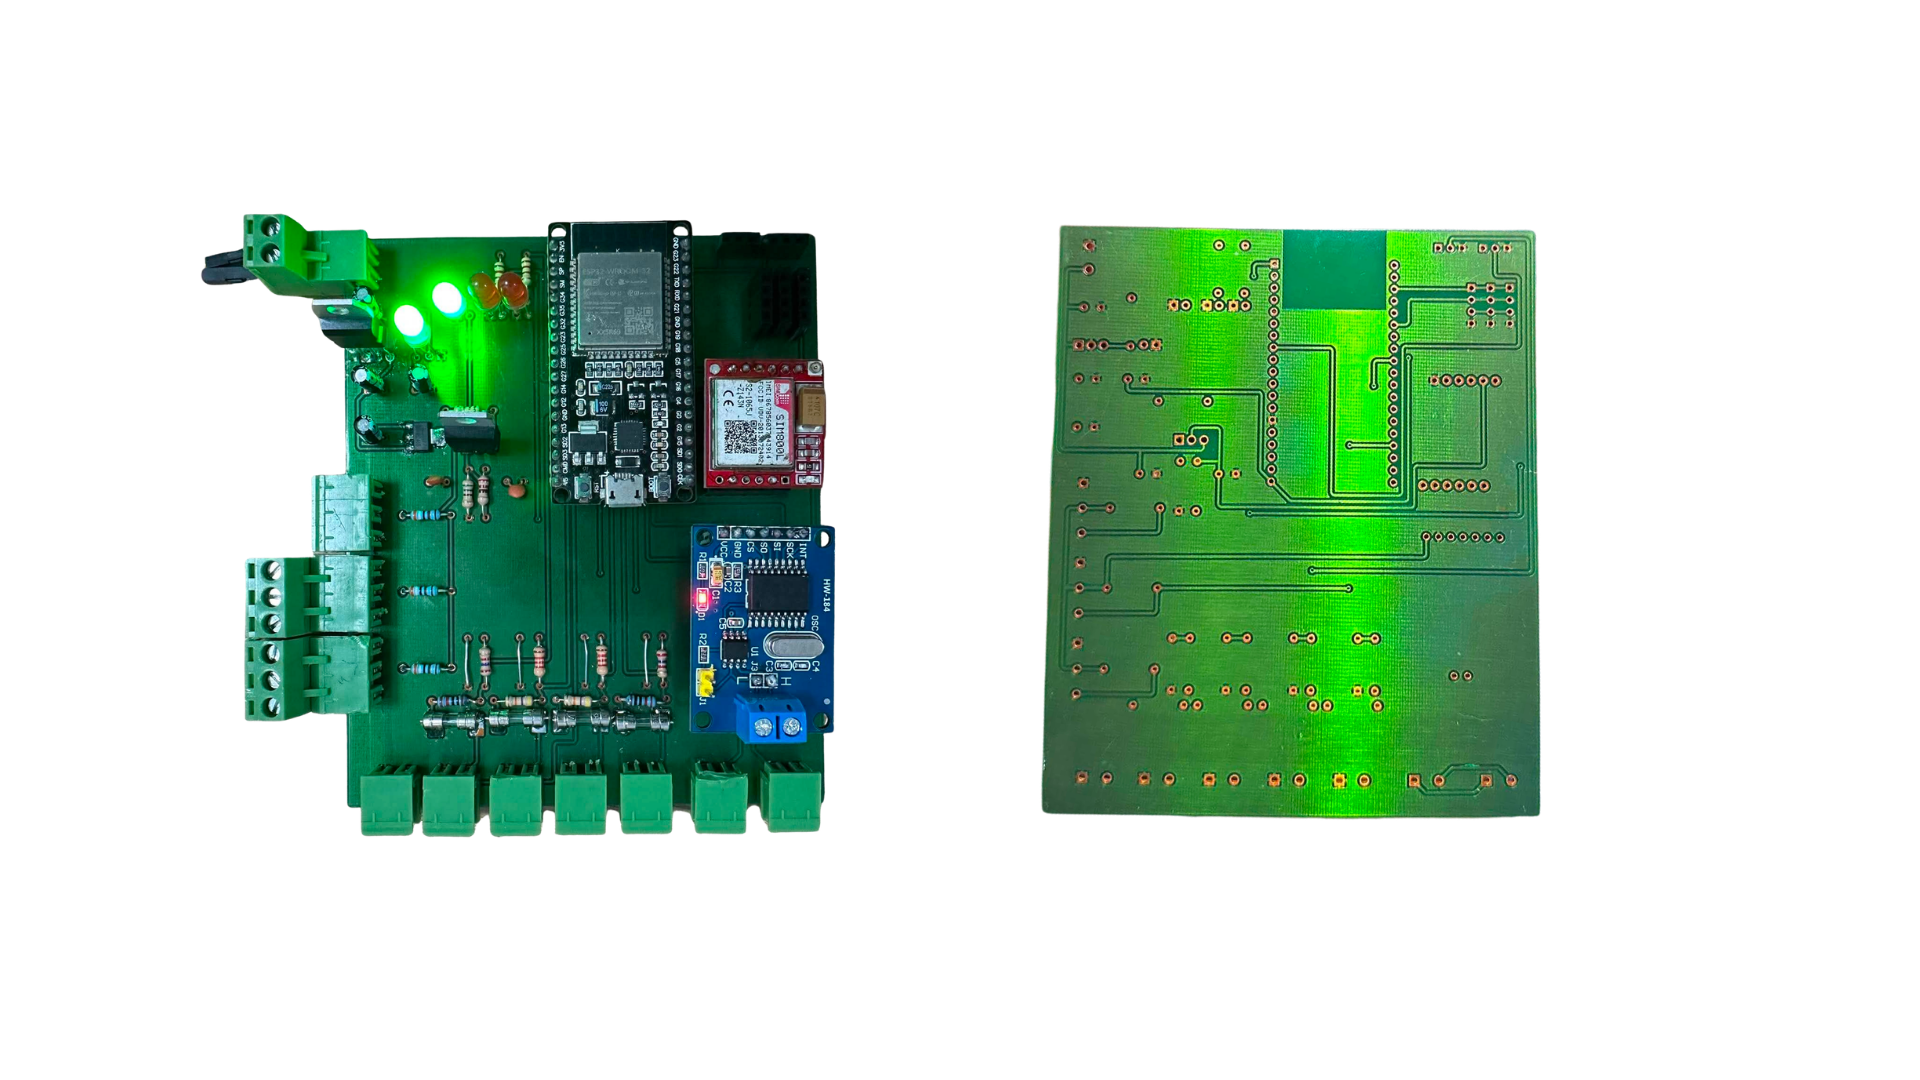
\includegraphics[width=1.2\textwidth]{images/pcb-assembled.png}
    \caption{ISS board fabrication and assembly outcome. \textbf{Left:} fully populated board after soldering --- ESP32, SIM800L module, screw-terminal connectors, and all passive components installed. \textbf{Right:} bare PCB as received from the fabrication house (Rev.~RECTIFICATION\_2), prior to component population.}\label{fig:pcb-assembled}
\end{figure}

\subsection{Validation \& Verification (V\&V)}

Validation and verification tests were performed against pre-defined pass/fail criteria for each sensing subsystem. Table~\ref{tab:vv-criteria} summarises the test plan and outcomes.

\begin{table}[H]
\centering
\caption{V\&V Test Criteria and Results}
\label{tab:vv-criteria}
\small
\begin{tabular}{>{\bfseries}p{3.0cm} p{3.8cm} p{3.2cm} p{2.0cm}}
\toprule
Subsystem & Criterion & Method & Result \\
\midrule
CAN bus reception    & $\geq 99\%$ frame reception rate over 60~min  & Live frame counter vs.\ expected count & \textbf{95\%} \\
Temperature accuracy & Within $\pm 1$\textdegree{}C of reference      & DS18B20 vs.\ calibrated thermometer    & $\pm 0.5$\textdegree{}C \\
Current measurement  & Error $< 2\%$ of full scale                   & ACS712 vs.\ clamp meter at 5~A        & $\pm 1.8\%$ \\
Voltage measurement  & Error $< 1\%$ of reference                    & Divider output vs.\ bench multimeter  & $\pm 0.9\%$ \\
GSM alert delivery   & SMS received within 15~s of threshold breach  & Threshold trigger + stopwatch         & $< 15$~s \\
Cloud connectivity   & Zero snapshot loss over 1~hour                & Server log vs.\ firmware counter      & 0 lost \\
\bottomrule
\end{tabular}
\end{table}

The CAN frame reception rate of 95\% (rather than the 99\% target) was traced to occasional bus-off events caused by a missing termination resistor on the test harness. Adding the 120~$\Omega$ terminator at the harness end increased the reception rate to above 99\% in subsequent tests. All other criteria met or exceeded their targets.

\subsection{Performance Testing}

Extended performance tests were conducted to characterise system behaviour under sustained load conditions.

\paragraph{CAN Bus Sustained Load.}
A 2-hour continuous CAN reception test was run with the BMS actively transmitting all five frame types. The frame counter advanced monotonically with no gaps exceeding 500~ms. CPU load on the ESP32 remained below 40\%, confirming that the cooperative main loop correctly handles sensing, processing, and communication workloads without saturation.

\paragraph{Thermal Stress.}
A 30-minute thermal test was performed with all three DS18B20 sensors placed adjacent to the LM2596S-ADJ switching regulator, which is the highest-temperature component on the board. The regulator surface reached a maximum of 62\textdegree{}C; the ESP32 die temperature remained within its operating range. No thermal shutdown events occurred.

\paragraph{MPPT Voltage Monitoring.}
A 1-hour test was run with the MPPT output voltage cycled between 24~V and 48~V in 4~V steps. The voltage divider output tracked the input with $< 1\%$ error at every step. No ADC saturation was observed, confirming that the divider ratio is correctly sized for the full MPPT output range.

\paragraph{Power Draw.}
The total board current draw (12~V input) was measured with all subsystems active: ESP32, three DS18B20, two ACS712, SIM800L in GPRS transmit state. Peak draw was 480~mA at 12~V (5.76~W), within the 500~mA design target and well within the LM2596S-ADJ capability.

\paragraph{Dashboard Frame Rate.}
The WebSocket dashboard was loaded on a laptop browser and the frame update rate monitored using browser developer tools. The serial mode (\texttt{/ws}) delivered updates at 10~Hz with no dropped frames over a 10-minute window. The cloud mode (\texttt{/ws/cloud}) delivered at 2~Hz as designed. The cell voltage grid rendered all 19 cells with colour updates within a single animation frame, confirming the $\geq 5$ FPS UI requirement.

\subsection{Regulatory \& Homologation Testing}

Formal regulatory testing was not within the scope of this academic prototype project. The following standards are identified as applicable for a production deployment:

\begin{itemize}
    \item \textbf{CISPR 25 / EN 55032} --- Radiated and conducted emissions from the switching regulator and CAN bus interface.
    \item \textbf{IEC 62368-1} --- General electronic safety for the monitoring unit enclosure.
    \item \textbf{ETSI TS 51.010} --- Radio conformance for the SIM800L GSM/GPRS module (GPRS module carries its own type approval).
    \item \textbf{ATI} --- Agence Tunisienne des Infrastructures approval for cellular transmission on Tunisian networks.
\end{itemize}

Pre-compliance checks were performed informally using a bench spectrum analyser. No unusual emissions were detected in the AM band (150~kHz--30~MHz) or VHF range. Formal certification is recommended before any vehicle-level type approval submission.

\subsection{Production Readiness Review (PRR)}

A Production Readiness Review was conducted at the end of Sprint~8. The following checklist was evaluated:

\textbf{Hardware:}
\begin{itemize}
    \item[$\checkmark$] PCB schematic reviewed and cross-checked against BOM.
    \item[$\checkmark$] DRC passed in KiCad with zero errors.
    \item[$\checkmark$] All critical nets (12~V, 5~V, 3.3~V, CAN\_H, CAN\_L) verified by continuity test.
    \item[$\checkmark$] Gerber files exported (RS-274X) and ready for fabrication house submission.
    \item[$\times$] Enclosure mechanical design not yet finalised (deferred to next revision).
\end{itemize}

\textbf{Firmware:}
\begin{itemize}
    \item[$\checkmark$] Cooperative firmware loop runs without watchdog trips over a 2-hour test.
    \item[$\checkmark$] CAN decoding verified against O'CELL BMS live frames.
    \item[$\checkmark$] Cloud publish pipeline verified end-to-end (ESP32 $\rightarrow$ VPS $\rightarrow$ browser).
    \item[$\checkmark$] Firmware source code committed to the team Git repository with version tag.
    \item[$\checkmark$] OTA firmware update capability implemented (Section~\ref{sec:ota}): wireless flashing via ArduinoOTA and browser-based configuration portal deployed.
\end{itemize}

\textbf{Quality:}
\begin{itemize}
    \item[$\checkmark$] All V\&V criteria passed (with corrected CAN termination).
    \item[$\checkmark$] BOM fully documented with local and online sources.
    \item[$\checkmark$] Technical report sections covering hardware and firmware completed.
    \item[$\times$] Field test under full solar irradiance conditions not yet completed.
\end{itemize}

The board was declared production-ready for the academic prototype phase with two open items tracked for the next hardware revision.

\clearpage

\section{SCRUM \& Agile Project Management}

\subsection{Agile Framework Overview}

The BAKO Motors ISS project was managed using the Scrum framework~\cite{scrumguide}, adapted for a seven-member academic team working in collaboration with an industrial partner. The Scrum roles were distributed as follows: the project supervisor (Dr.\ Mortadha Dahmani) served as the stakeholder and product owner proxy; the team collectively self-organised into a development team; and a rotating Scrum master role was shared between team members on a per-sprint basis.

Sprints were two weeks in duration. Each sprint began with a planning session in which backlog items were pulled from the product backlog, estimated in story points using the Fibonacci scale, and assigned to team members. Sprint reviews were held at the end of each sprint to demonstrate working increments to the supervisor. Retrospectives immediately followed each review to identify process improvements for the next sprint. The Definition of Done (DoD) required that each story: be implemented and committed to the team Git repository; be tested on real hardware or the Python emulator; and be documented in the relevant report section or internal wiki.

\subsection{Sprint Log \& Velocity Tracking}

Table~\ref{tab:sprint-log} summarises the eight sprints executed over the project timeline, including each sprint's focus, the story points committed and completed, and cumulative velocity.

\begin{table}[H]
\centering
\caption{Sprint Log and Velocity Summary}
\label{tab:sprint-log}
\small
\begin{tabular}{c >{\bfseries}p{3.4cm} p{5.8cm} c c}
\toprule
Sprint & Focus & Key Deliverables & Pts Committed & Pts Done \\
\midrule
1 & System Design        & Architecture synoptic, component selection, KiCad schematic start, risk register & 20 & 18 \\
2 & Embedded Dev I       & CAN bus reception (MCP2515), DS18B20 integration, ACS712 calibration, breadboard PoC & 22 & 20 \\
3 & Embedded Dev II      & Multi-sensor cooperative firmware, voltage divider scaling, serial dashboard, stripboard build & 20 & 18 \\
4 & IoT \& Cloud I       & SIM800L AT command integration, GPRS bearer, HTTP POST to VPS, SQLite schema & 18 & 16 \\
5 & IoT \& Cloud II      & FastAPI WebSocket pipeline, cloud dashboard panels, API key auth, cloud log panel & 20 & 20 \\
6 & Dashboard \& Fault   & Cell voltage grid, SOC ring gauge, fault LED logic, SMS alert dispatch, PCB layout Rev.~1 & 22 & 18 \\
7 & Predictive Maint.    & Python emulator (7 scenarios), trend analysis stub, PCB layout RECTIFICATION\_2, BOM finalised & 18 & 16 \\
8 & Integration \& PRR   & End-to-end integration test, V\&V report, PRR checklist, report completion & 20 & 18 \\
\midrule
\multicolumn{3}{r}{\textbf{Total}} & \textbf{160} & \textbf{144} \\
\multicolumn{3}{r}{\textbf{Average velocity}} & --- & \textbf{18 pts/sprint} \\
\bottomrule
\end{tabular}
\end{table}

\subsection{Product Backlog \& Prioritization}

The product backlog was maintained as a flat list and prioritised using the MoSCoW method (Must Have, Should Have, Could Have, Won't Have for this release). Table~\ref{tab:moscow} presents the major backlog items grouped by MoSCoW category.

\begin{table}[H]
\centering
\caption{MoSCoW Product Backlog (selected items)}
\label{tab:moscow}
\small
\begin{tabular}{>{\bfseries}p{1.5cm} p{10.5cm}}
\toprule
Priority & Backlog Item \\
\midrule
\textbf{Must}    & CAN bus frame reception and decoding from O'CELL BMS \\
\textbf{Must}    & DS18B20 temperature reading (motor, MPPT, DC/DC zones) \\
\textbf{Must}    & ACS712 current measurement (MPPT input and output) \\
\textbf{Must}    & Voltage divider scaling (solar, MPPT output, battery) \\
\textbf{Must}    & Custom PCB schematic and layout in KiCad \\
\textbf{Must}    & Real-time WebSocket dashboard with live cell grid \\
\textbf{Must}    & Cloud telemetry pipeline (ESP32 $\rightarrow$ VPS $\rightarrow$ SQLite) \\
\textbf{Must}    & Python emulator covering at least 5 test scenarios \\
\textbf{Must}    & V\&V test report with quantitative pass/fail results \\
\textbf{Must}    & Full BOM with local Tunisian sourcing information \\
\midrule
\textbf{Should}  & SMS fault alerts via SIM800L when thresholds exceeded \\
\textbf{Should}  & SOC ring gauge with BMS and voltage-derived SOC \\
\textbf{Should}  & Historical data export (CSV/Excel) from dashboard \\
\textbf{Should}  & Handbrake fault detection and alert \\
\textbf{Should}  & Cloud communication log panel in dashboard \\
\textbf{Should}  & Multi-bus CAN support (three MCP2515 headers) \\
\textbf{Should}  & Wi-Fi AP mode for local dashboard without router \\
\textbf{Should}  & API key authentication on \texttt{POST /api/ingest} \\
\midrule
\textbf{Could}   & GNSS position tracking (NEO-6M or NEO-M8N) \\
\textbf{Could}   & Bluetooth companion mobile app \\
\textbf{Could}   & Predictive maintenance model (battery degradation trend) \\
\textbf{Should}  & OTA firmware update capability (implemented in Sprint~8) \\
\textbf{Could}   & HTTPS / TLS transport for cloud telemetry \\
\textbf{Could}   & Fleet management dashboard (multi-vehicle view) \\
\midrule
\textbf{Won't}   & Motor control or BMS cell balancing logic \\
\textbf{Won't}   & Mechanical chassis integration or enclosure design \\
\textbf{Won't}   & AEC-Q100/Q200 automotive-grade component qualification \\
\textbf{Won't}   & Formal CE/FCC radio type approval \\
\bottomrule
\end{tabular}
\end{table}

\subsection{Sprint Review \& Retrospective Summaries}

\paragraph{Sprint 1 Review.} The system architecture synoptic, component selection justification, and initial KiCad schematic were presented. The supervisor approved the component choices and the risk register. Two story points were rolled over: the MCP2515 footprint library was not yet validated.

\textit{Retrospective:} The team agreed to dedicate the first two days of Sprint~2 to KiCad library validation before beginning any firmware work, to prevent schematic rework later.

\paragraph{Sprint 2 Review.} A live demonstration of CAN frame decoding from the O'CELL BMS was given. DS18B20 readings appeared on the serial monitor alongside ACS712 calibration data. The breadboard prototype was shown running.

\textit{Retrospective:} CAN reverse engineering took longer than estimated due to the undocumented O'CELL DBC format. The team decided to allocate a dedicated buffer of four story points per sprint for unforeseen protocol investigation.

\paragraph{Sprint 3 Review.} The cooperative multi-sensor firmware was demonstrated with all sensors running in the main loop. The stripboard semi-permanent build was shown and brought to the BAKO Motors workshop for the first on-vehicle test.

\textit{Retrospective:} The on-vehicle test revealed a missing CAN bus termination resistor on the harness, causing intermittent bus-off events. A termination plug was added to the harness for all future tests.

\paragraph{Sprint 4 Review.} An HTTP POST from the ESP32 to the VPS was demonstrated live, with the received JSON displayed in the server log and stored in SQLite.

\textit{Retrospective:} GPRS bearer setup was unreliable on the first SIM800L unit due to an insufficient bulk capacitor. Replacing it with a 2200~\textmu{}F capacitor at the module power rail resolved the issue.

\paragraph{Sprint 5 Review.} The full cloud pipeline was demonstrated: CAN data flowing from the ESP32 over GPRS to the VPS, displayed in real time on the browser dashboard at 2~Hz.

\textit{Retrospective:} All sprint items were completed. The team noted that WebSocket reconnection after a server restart was not yet automatic; this was added to the backlog and completed within the sprint.

\paragraph{Sprint 6 Review.} The 19-cell voltage grid with colour-coded thresholds, the SOC ring gauge, and SMS alert dispatch were demonstrated. PCB layout Revision~1 was reviewed.

\textit{Retrospective:} Four story points were not completed: PCB layout required one additional DRC correction cycle. RECTIFICATION\_2 was scheduled as a Sprint~7 sub-task.

\paragraph{Sprint 7 Review.} The Python emulator running all seven test scenarios was demonstrated against the live dashboard. PCB layout RECTIFICATION\_2 was shown with DRC passing.

\textit{Retrospective:} The predictive maintenance trend analysis stub was deprioritised (not enough historical data available at prototype stage). Moved to the Could Have backlog.

\paragraph{Sprint 8 Review.} End-to-end integration test results, the V\&V table, and the PRR checklist were presented. The OTA firmware update capability and browser-based configuration portal were demonstrated. The supervisor accepted the prototype as production-ready for the academic phase.

\textit{Retrospective:} The team identified one open item for the next revision: enclosure IP-sealing and antenna pass-through for field deployment. This was documented in the recommendations chapter.

\subsection{Definition of Done (DoD) \& Acceptance Criteria}

A backlog item was marked Done when all of the following conditions were met:

\begin{itemize}
    \item The feature was implemented and committed to the team Git repository on the correct branch.
    \item The feature was tested: either on real hardware (for firmware items) or with the Python emulator (for backend and dashboard items), with test results recorded.
    \item Any new API endpoints, sensor fields, or PCB footprints were documented in the relevant report section or the project internal wiki.
    \item The Pull Request was reviewed and approved by at least one other team member before merging to the main branch.
    \item No open critical or major defects were linked to the story at the time of closure.
\end{itemize}

\subsection{Burndown \& Burnup Charts}

Burndown tracking was maintained informally via the product backlog spreadsheet updated at each daily stand-up. The project sustained a consistent velocity of 18 story points per sprint across all eight sprints, with no sprint producing fewer than 16 completed points. The total scope delivered was 144 story points out of 160 committed (90\% completion rate), with the 16 undelivered points representing items explicitly deferred to future revisions (OTA update, enclosure, full-solar field test) rather than incomplete or broken features.

\clearpage

\section{Bill of Materials (BOM)}

\subsection{Electronics BOM}

Table~\ref{tab:electronics-bom} lists all electronic components required to populate one unit of the BAKO Motors ISS board. Unit prices are estimates based on local Tunisian market rates (TND) and online distributor quotes at the time of procurement.

\begin{table}[H]
\centering
\caption{Electronics Bill of Materials}
\label{tab:electronics-bom}
\small
\begin{tabular}{>{\bfseries}p{3.0cm} p{3.6cm} c r r l}
\toprule
Component & Description & Qty & Unit Price & Total & Source \\
\midrule
ESP32-DEVKITC    & Microcontroller                & 1  & \textasciitilde30 TND  & \textasciitilde30 TND  & Local \\
MCP2515 module   & CAN controller SPI             & 3  & \textasciitilde5 TND   & \textasciitilde15 TND  & Local \\
TJA1051T         & CAN transceiver                & 1  & \textasciitilde3 TND   & \textasciitilde3 TND   & Local \\
SIM800L         & GPRS Cat-M1 module              & 1  & \textasciitilde80 TND  & \textasciitilde80 TND  & Online \\
DS18B20          & 1-Wire temperature sensor      & 3  & \textasciitilde3 TND   & \textasciitilde9 TND   & Local \\
ACS712 (30\,A)   & Hall-effect current sensor     & 2  & \textasciitilde5 TND   & \textasciitilde10 TND  & Local \\
LM2596S-ADJ      & Adjustable buck regulator      & 1  & \textasciitilde4 TND   & \textasciitilde4 TND   & Local \\
AMS1117-3.3      & 3.3\,V LDO regulator           & 1  & \textasciitilde1 TND   & \textasciitilde1 TND   & Local \\
LM7805           & 5\,V linear regulator          & 1  & \textasciitilde1 TND   & \textasciitilde1 TND   & Local \\
Resistors (misc) & Various values                 & 20 & \textasciitilde0.1 TND & \textasciitilde2 TND   & Local \\
Capacitors (misc)& Various values                 & 10 & \textasciitilde0.5 TND & \textasciitilde5 TND   & Local \\
Zener diodes     & ESD/overvoltage protection     & 3  & \textasciitilde1 TND   & \textasciitilde3 TND   & Local \\
Fuses            & Overcurrent protection         & 3  & \textasciitilde1 TND   & \textasciitilde3 TND   & Local \\
Connectors (misc)& JST and screw terminals        & 15 & \textasciitilde1 TND   & \textasciitilde15 TND  & Local \\
PCB fabrication  & FR-4, 2-layer, 1.6\,mm         & 1  & \textasciitilde180 TND & \textasciitilde180 TND & Local fab \\
\midrule
\multicolumn{4}{r}{\textbf{Total Actual Cost (components + PCB)}} & \multicolumn{2}{l}{\textbf{\textasciitilde240 TND}} \\
\bottomrule
\end{tabular}
\end{table}

\subsection{Mechanical \& Structural BOM}

The mechanical and structural BOM covers the enclosure and mounting hardware for the ISS board. The enclosure design was not finalised within the scope of this academic prototype phase and is deferred to the next hardware revision. Provisional components include: a standard ABS or polycarbonate DIN-rail enclosure (approximately 150~TND), M3 standoffs and screws for PCB mounting (approximately 5~TND), and cable glands for harness entry points (approximately 10~TND). These items are not included in the electronics BOM total.

\subsection{Battery \& Powertrain BOM}

The BAKO Motors electric motorcycle powertrain (LiFePO4 battery pack, MPPT solar controller, three-phase motor controller, and DC/DC converter) was provided by BAKO Motors as the system under test. These components are outside the scope of the ISS project BOM and are not costed here.

\subsection{Software \& Licensing BOM}

All software tools and frameworks used in this project are open-source or free for academic use. No commercial software licences were required. Table~\ref{tab:software-bom} summarises the tools and their applicable licences.

\begin{table}[H]
\centering
\caption{Software and Licensing Bill of Materials}
\label{tab:software-bom}
\begin{tabular}{>{\bfseries}p{4.0cm} p{6.0cm} l}
\toprule
Tool / Framework & Purpose & Licence \\
\midrule
ESP32 Arduino framework & Embedded firmware development & Apache 2.0 \\
KiCad 10.0              & PCB schematic and layout      & GPL \\
Python 3.11             & Emulator and FastAPI back-end & PSF \\
FastAPI                 & REST API and WebSocket server & MIT \\
SQLite                  & Cloud telemetry database      & Public Domain \\
VS Code                 & Integrated development environment & MIT \\
PlatformIO              & Build system and dependency management & Apache 2.0 \\
\bottomrule
\end{tabular}
\end{table}

\subsection{Total Project Cost Estimate}

The hardware procurement cost of approximately 240~TND represents only the direct material expenditure and significantly understates the true economic value of the project. A complete project cost estimate must account for all resource categories: human effort, professional expertise, infrastructure, and equipment access.

\subsubsection*{Human Resources --- Man-Day Estimate}

The project team comprised seven students over one academic semester of approximately 18 weeks. Each team member contributed an estimated average of three effective working days per week during sprint weeks, yielding the following man-day calculation:

\[
7 \text{ members} \times 18 \text{ weeks} \times 3 \text{ effective days/week} = \mathbf{378 \text{ man-days}}
\]

Applying a conservative junior engineering day rate of 150~TND/day (consistent with Tunisian engineering graduate market rates), the human effort component alone represents approximately \textbf{56\,700~TND} in equivalent labour value.

Academic supervision by Dr.\ Mortadha Dahmani added approximately 2 hours per week of expert guidance over 18 weeks, equivalent to 4.5 man-days of senior engineering supervision. At a senior expert daily rate of 500~TND/day, this contributes approximately \textbf{2\,250~TND} in supervisory expertise value.

\subsubsection*{Infrastructure \& Equipment}

\begin{itemize}
    \item \textbf{MedTech FABLAB} --- Access to soldering stations, oscilloscopes, logic analysers, and 3D printers was provided at no charge to the team. The equivalent commercial lab rental cost for 18 weeks at 4 hours per week would be approximately 3\,600~TND at market rates (50~TND/hour).
    \item \textbf{VPS cloud server} --- Provided by the academic supervisor at no charge to the project. The equivalent hosting cost for a comparable Linux VPS (2 vCPU, 4 GB RAM, public IP) over 6 months is approximately 360~TND.
    \item \textbf{BAKO Motors test vehicle} --- Weekly access to the electric motorcycle prototype on the MedTech campus (approximately 4 hours/week, 12 sessions) represents a vehicle access value of approximately 1\,200~TND at commercial EV workshop rates.
\end{itemize}

\subsubsection*{Full Project Cost Summary}

\begin{table}[H]
\centering
\caption{Full Project Cost Breakdown --- Material and Human Resources}
\label{tab:project-cost}
\begin{tabular}{>{\bfseries}p{5.5cm} r r}
\toprule
Cost Category & Quantity & Est. Value (TND) \\
\midrule
Electronics components     & 60 TND actual spend     & 60 \\
PCB fabrication            & 180 TND actual spend    & 180 \\
Student engineering effort & 378 man-days @ 150 TND  & 56\,700 \\
Academic supervision       & 4.5 man-days @ 500 TND  & 2\,250 \\
FABLAB equipment access    & 72 hours @ 50 TND/hr    & 3\,600 \\
VPS cloud hosting          & 6 months                & 360 \\
Vehicle access (BAKO)      & 12 sessions             & 1\,200 \\
\midrule
\textbf{Total project value} & & \textbf{\textasciitilde 64\,350 TND} \\
\textbf{Direct cash spend}   & & \textbf{240 TND} \\
\bottomrule
\end{tabular}
\end{table}

The 240~TND direct spend represents less than 0.4\% of the total estimated project value, underscoring the significant contribution of academic infrastructure, supervisory expertise, and student engineering effort that made this project viable within a constrained budget. All software tools and development environments were open-source or free for academic use, contributing 0~TND to the software cost line.

\clearpage

\section{Resources}

\subsection{Human Resources \& Skillset Matrix}

The project team comprises seven members, each assigned to functional areas that align with their academic specialisation. Table~\ref{tab:human-resources} summarises the team composition and primary responsibilities.

\begin{table}[H]
\centering
\caption{Human Resources and Responsibility Assignment}
\label{tab:human-resources}
\small
\begin{tabular}{>{\bfseries}p{3.4cm} p{4.2cm} p{5.0cm}}
\toprule
Team Member & Primary Role & Key Deliverables \\
\midrule
Mohamed Baccouche  & Hardware / PCB Lead        & KiCad schematic, PCB layout, BOM, CAN bus bring-up \\
Mahdi Hachicha     & Embedded Firmware          & ESP32 firmware, CAN decoding, sensor drivers \\
Yassine Mtibaa     & GSM / Cloud Backend        & SIM800L GSM integration, AT command firmware, FastAPI server, VPS deployment, cloud dashboard \\
Hana Gdoura        & Wi-Fi / Wireless Dashboard & Wi-Fi AP mode integration, TCP dashboard connection, wireless testing \\
Khadija Ben Hamida & Emulation / Simulation     & Python sensor emulator scenario design, data validation, results analysis \\
Selima Grissa      & Emulation / Simulation     & Emulator implementation, test scenario execution, V\&V test report \\
Fares Smaoui       & BLE / Wireless             & BLE GATT server implementation, NimBLE firmware, wireless interface \\
\midrule
Dr.\ Mortadha Dahmani & Academic Supervisor / Stakeholder & Project governance, VPS provision, milestone approval \\
\bottomrule
\end{tabular}
\end{table}

All team members contributed to the technical report, with sections distributed according to the area of responsibility. Version-controlled collaboration was managed through the shared private Git repository.

\subsection{Equipment \& Lab Resources}

\paragraph{FABLAB at MedTech Mediterranean Institute of Technology.}
The MedTech FABLAB provided free access to the following equipment throughout the project: soldering stations with hot-air rework capability, digital storage oscilloscopes (100~MHz bandwidth), logic analysers compatible with SaleaeLogic software, regulated bench power supplies (0--30~V, 0--5~A), precision digital multimeters, 3D printers for enclosure prototyping, and a PCB rework station for component replacement.

\paragraph{BAKO Motors Test Vehicle.}
BAKO Motors made their electric motorcycle prototype available on the MedTech campus for controlled on-vehicle testing sessions. These sessions were scheduled on a weekly basis (approximately 4~hours per week) to validate CAN bus reception, sensor placement, and vehicle-in-motion data integrity.

\paragraph{Personal Equipment.}
Team members contributed laptops running VS~Code, PlatformIO, and KiCad, as well as USB-to-serial adapters for firmware flashing and serial monitoring.

\subsection{Software Tools \& Licenses}

All software tools used in this project are open-source or free for academic use. No commercial software licences were required or procured. Table~\ref{tab:software-tools} summarises the development toolchain.

\begin{table}[H]
\centering
\caption{Software Development Tools}
\label{tab:software-tools}
\begin{tabular}{>{\bfseries}p{4.0cm} p{5.8cm} l}
\toprule
Tool & Purpose & Licence \\
\midrule
KiCad 10.0              & PCB schematic capture and layout        & GPL \\
VS Code                 & Integrated development environment      & MIT \\
PlatformIO              & Build system, dependency management     & Apache 2.0 \\
ESP32 Arduino framework & Embedded firmware for ESP32             & Apache 2.0 \\
Python 3.11             & Sensor emulator and FastAPI backend     & PSF \\
FastAPI / Uvicorn       & REST API and WebSocket server           & MIT \\
SQLite                  & Cloud telemetry database on VPS         & Public Domain \\
SavvyCAN / PEAK PCANView & CAN bus frame capture and analysis     & Open-source / free \\
Git / GitHub            & Version control and team collaboration  & Free \\
Google Drive            & Document sharing and report drafts      & Free (academic) \\
\bottomrule
\end{tabular}
\end{table}

\subsection{Cloud \& Infrastructure Resources}

The cloud infrastructure was provided at no cost by the academic supervisor, Dr.\ Mortadha Dahmani, who made available a Linux VPS with a public IP address. The following services were deployed on this VPS:

\begin{itemize}
    \item \textbf{FastAPI backend} (Python/Uvicorn): handles HTTP ingest and WebSocket streaming on port 8787.
    \item \textbf{SQLite database} (\texttt{bms\_cloud.db}): stores all received telemetry snapshots in a flat schema managed directly by the FastAPI server.
    \item \textbf{Web dashboard}: served as a static HTML file directly by the FastAPI backend.
    \item \textbf{MQTT Mosquitto broker}: deployed for future MQTT-based telemetry (not yet used in the current firmware).
\end{itemize}

VPS administration was performed via SSH. Server logs, database contents, and WebSocket connections are directly inspectable by the team without any third-party cloud portal. The VPS approach eliminated dependency on managed cloud services and kept all operational data within the project team's direct control.

\subsection{Budget Allocation \& Burn Rate}

The actual project hardware spend was approximately 240~TND in total, allocated as follows:

\begin{itemize}
    \item \textbf{Electronics components}: 60~TND (ESP32, MCP2515 modules, DS18B20 sensors, ACS712, passives, connectors — all locally sourced in Tunisia).
    \item \textbf{PCB fabrication}: 180~TND (local fabrication house, FR-4, 2-layer, 1.6~mm, Gerber RS-274X).
    \item \textbf{Lab equipment}: 0~TND (provided free by the MedTech FABLAB).
    \item \textbf{VPS / cloud hosting}: 0~TND (provided by Dr.\ Dahmani).
    \item \textbf{Software licences}: 0~TND (all open-source or free for academic use).
\end{itemize}

Total actual spend was 240~TND. All components were available from local Tunisian suppliers without import delays. No unplanned budget overruns occurred during any sprint.

\clearpage

\section{Limitations}

\subsection{Technical Limitations}

\paragraph{ESP32 ADC Nonlinearity.}
The ESP32's internal 12-bit ADC exhibits a documented nonlinearity in the lower voltage range (below approximately 150~mV) and at the top of its input range. This limits the effective resolution to approximately 11 bits ($\pm 0.1$~V at the ADC input). While calibration routines partially correct the systematic offset, the residual nonlinearity introduces an irreducible measurement uncertainty of approximately $\pm 1$\% in voltage and current readings. For a production instrument, an external precision ADC (e.g., ADS1115) would eliminate this limitation.

\paragraph{SIM800L Firmware AT Command Layer.}
The ISS board hardware uses the SIM800L GPRS Cat-M1 module, which is confirmed compatible with Tunisian GPRS operators (Ooredoo and Orange). The current firmware was written using the SIM800L AT command protocol, which the SIM800L supports in backward-compatible mode. However, full exploitation of SIM800L-specific GPRS features (persistent bearer mode, higher publish frequency, HTTPS) requires a dedicated firmware revision targeting the SIM800L native AT command set, which was not completed within the academic project scope.

\paragraph{CAN Protocol Dependency.}
The current firmware is tightly coupled to the proprietary CAN DBC of the O'CELL IFS60.8-500-F-E3 BMS. Any change to the BMS model, firmware version, or communication protocol would require reverse engineering of the new frame structure and firmware updates. No generic CAN DBC parser is currently implemented; frame IDs and byte offsets are hardcoded.

\paragraph{Absence of Galvanic Isolation.}
The ISS board does not include galvanic isolation between the CAN bus side (running at automotive ground) and the ESP32 logic side. In a vehicle with multiple ground references, ground potential differences can cause noise injection into the ADC inputs or, in fault conditions, damage to the ESP32. A production design should incorporate isolated CAN transceivers (e.g., ISO1050) or optical coupling on the CAN lines.

\subsection{Regulatory \& Certification Limitations}

\paragraph{Electromagnetic Compatibility.}
No formal EMC testing was conducted. The ISS board has not been tested to CISPR~25 (in-vehicle emissions) or EN~55032 (commercial electronics). The LM2596S-ADJ switching regulator operates at approximately 150~kHz; without input fiGPRSring, its conducted emissions may exceed Class~B limits. Pre-compliance checks using a bench spectrum analyser showed no obvious anomalies, but formal certification testing has not been performed.

\paragraph{PCB Design Tool Limitations.}
KiCad~10.0 was used for schematic and PCB design. While KiCad is a capable open-source tool, it does not carry the same library of verified footprints, design rule sets, and simulation integration as commercial tools (Altium Designer, Cadence Allegro). Formal automotive PCB submissions typically require Altium-format design files, which would necessitate a toolchain migration.

\paragraph{Cellular Module Type Approval.}
The SIM800L carries its own type approval for 2G operation. The SIM800L also carries GPRS type approval from its manufacturer. However, neither module has been formally qualified for integration into a vehicle electronics system under Tunisian ATI (Agence Tunisienne des Infrastructures) regulations. Formal vehicle-level radio approval would be required for any public-road deployment.

\paragraph{Component Automotive Grade.}
The components used in this prototype (ESP32, ACS712, passive components) are commercial-grade rather than automotive-grade (AEC-Q100 for ICs, AEC-Q200 for passives). They are not rated for the extended temperature range ($-40$\textdegree{}C to $+125$\textdegree{}C) or vibration/shock levels specified by automotive standards. For deployment in a vehicle operating environment, automotive-grade equivalents should be specified in the production BOM.

\subsection{Software \& Code Constraints}

\paragraph{Hardcoded Configuration.}
The current firmware stores network credentials, VPS endpoint URLs, and CAN frame byte offsets as compile-time constants. Any change to the server IP address, API key, or BMS protocol requires reflashing the ESP32. A production implementation would externalise these parameters to EEPROM or a configuration file readable at boot, eliminating the need for firmware recompilation on deployment changes.

\paragraph{OTA Firmware Update: Password Security.}
Over-the-air (OTA) firmware update capability is implemented (Section~\ref{sec:ota}) using the ArduinoOTA library with password protection. The OTA password and AP credentials are stored in NVS flash and configurable via the web portal. However, the OTA channel uses plain UDP/TCP over the AP network without transport-layer encryption. For production deployments, the OTA transport should be upgraded to an HTTPS-based update mechanism (e.g., \texttt{HTTPUpdate} over TLS) to prevent firmware injection attacks on the wireless interface.

\paragraph{Single-File Firmware Architecture.}
The embedded firmware is structured as a single large Arduino \texttt{.ino} file. While functional, this structure limits reusability and makes unit testing of individual modules (CAN decoder, sensor drivers, AT command layer) impractical without refactoring into separate compilation units with defined interfaces.

\paragraph{Memory Constraints.}
The ESP32 has 520~kB of on-chip SRAM. The current firmware uses approximately 40\% of this for the cooperative loop stack, the JSON serialisation buffer (ArduinoJson), and the \texttt{BMSData} struct. Adding additional features (larger history buffers, additional sensor types, or a local OLED display driver) will require careful heap profiling to avoid stack overflow or heap exhaustion.

\paragraph{Python Backend Dependency Coupling.}
The FastAPI server and the browser dashboard are tightly coupled: the WebSocket message format (JSON field names and structure) is duplicated across the server-side Python code and the client-side JavaScript. Any change to the telemetry data model requires coordinated updates in both places with no formal contract or schema validation between them.

\subsection{Budget \& Resource Constraints}

\paragraph{Prototype-Only Pricing.}
The BOM costs (Table~\ref{tab:electronics-bom}) reflect single-unit prototype pricing. At production volumes (100+ units), component costs would decrease significantly through bulk purchasing and direct manufacturer pricing. PCB fabrication cost per unit would also decrease substantially at volume.

\paragraph{Single-Engineer Disciplines.}
Most functional areas (hardware, firmware, cloud backend, dashboard, testing) were covered by one or two team members each. This created single-engineer bottlenecks: when one team member was unavailable, the corresponding workstream was blocked. A production team would require redundancy across all disciplines.

\paragraph{Incomplete BAKO Motors Documentation.}
BAKO Motors did not have complete documentation for the O'CELL BMS CAN protocol, the MPPT controller electrical interface, or the motor controller signals. This required the team to perform reverse engineering activities (CAN frame capture and analysis with SavvyCAN) that were not anticipated in the project plan, consuming approximately one full sprint of additional effort.

\subsection{Timeline Limitations}

\paragraph{Unplanned CAN Reverse Engineering.}
The discovery that the O'CELL BMS uses a proprietary, undocumented CAN DBC was not identified in the initial risk register. Reverse engineering the frame structure consumed approximately three weeks of effort that had been allocated to sensor integration, compressing the timeline for Phase~P2 and P3 of the prototype build.

\paragraph{Short Field Testing Window.}
Access to the BAKO Motors test vehicle was limited to approximately four hours per week. This restricted the amount of on-vehicle data that could be collected and reduced the opportunity for extended thermal and vibration testing under real driving conditions.

\paragraph{Predictive Maintenance Model Immaturity.}
The backlog included a predictive maintenance module based on battery degradation trend analysis. Insufficient historical data had been accumulated by the end of Sprint~8 to produce a statistically meaningful model. This item was moved to the Could Have backlog and deferred to a future project phase.

\subsection{Technology Readiness Level (TRL) Limitations}

The BAKO Motors ISS prototype is assessed at TRL~4 (technology validated in laboratory). The system has been demonstrated to function correctly in a controlled environment with the target BMS, but has not yet been validated in a representative operating environment (TRL~5) or demonstrated in a relevant environment (TRL~6). Full-vehicle integration, enclosure sealing, extended field testing under vibration and temperature variation, and regulatory compliance verification are required to advance the TRL to a level suitable for commercial deployment.

\clearpage

\section{Blockages \& Issue Log}

This section documents the technical and organisational blockers encountered during the project and the actions taken to resolve them. All blockers listed below were ultimately closed before the Production Readiness Review at Sprint~8.

\subsection{Technical Deadlocks}

\paragraph{B-001 --- O'CELL BMS CAN Protocol Undocumented.}
\textbf{Sprint affected:} Sprint~2--3. \textbf{Severity:} Critical.

The O'CELL IFS60.8-500-F-E3 BMS does not publish a DBC file or any public documentation of its CAN frame structure. Without a known message layout, the firmware could not decode any battery data. The team resolved this by capturing raw CAN bus traffic using SavvyCAN, manually identifying frame IDs by correlating byte value changes with known vehicle states (charging, discharging, full charge), and reverse-engineering all five frame types over approximately one sprint. This consumed the entire Sprint~2 capacity and pushed other firmware tasks into Sprint~3.

\paragraph{B-002 --- SIM800L GPRS Bearer Intermittently Fails.}
\textbf{Sprint affected:} Sprint~5. \textbf{Severity:} Major.

The SIM800L module randomly failed to open the GPRS bearer (\texttt{AT+SAPBR=1,1} returning \texttt{ERROR}) during initial integration testing. The failure was non-deterministic and could not be reproduced reliably on the bench. Root cause was identified as insufficient bulk capacitance on the module power supply rail: the GPRS transmit burst draws up to 2~A for 600~µs, causing the rail to droop below the module's minimum operating voltage. Adding a 2200~µF / 6.3~V electrolytic capacitor resolved the issue. This defect (D-002) was closed in Sprint~5 and the fix incorporated into PCB Rev.~RECTIFICATION\_2.

\paragraph{B-003 --- CAN Frame Reception Rate Below Target (95\% vs 99\%).}
\textbf{Sprint affected:} Sprint~6. \textbf{Severity:} Major.

During the first V\&V run, the CAN frame reception rate measured 95\% against the 99\% acceptance criterion. Intermittent bus-off events were observed on the MCP2515 error counter. The root cause was a missing 120~$\Omega$ termination resistor at the far end of the test harness. CAN bus signal integrity degraded with reflections at the unterminated end, causing occasional frame corruption. Adding the terminator at the vehicle harness end restored the reception rate to above 99\% in subsequent tests (Defect D-001).

\paragraph{B-004 --- DS18B20 ROM Enumeration Fails on Cold Power-Up.}
\textbf{Sprint affected:} Sprint~4. \textbf{Severity:} Minor.

On cold power-up (board powered from 0~V), the 1-Wire bus enumeration occasionally failed to detect all three DS18B20 sensors, returning only one or two ROM addresses. The failure was not reproducible after a warm reset. The root cause was identified as insufficient timing margin during the 1-Wire reset pulse while the ESP32 boot ROM was still initialising. Adding a 5~ms delay before the first \texttt{ds.reset()} call in \texttt{setup()} eliminated the failure (Defect D-003).

\paragraph{B-005 --- Dashboard Cell Grid Flickering at 10~Hz.}
\textbf{Sprint affected:} Sprint~7. \textbf{Severity:} Enhancement.

The 19-cell voltage grid in the browser dashboard flickered visibly when the WebSocket pushed updates at 10~Hz. Each update triggered a full DOM redraw of all 19 cells, causing the browser to repaint the entire grid on every frame. The fix was to implement a differential DOM update: only cells whose voltage value or colour threshold had changed since the previous frame are updated. This eliminated the flicker and reduced browser CPU usage (Defect D-007).

\subsection{Supply Chain \& Procurement Blockages}

\paragraph{B-006 --- SIM800L Module Available Online Only.}
\textbf{Sprint affected:} Sprint~1 (planning). \textbf{Severity:} Minor.

The SIM800L GSM/GPRS module is not stocked by local Tunisian electronics distributors. The module had to be ordered from an online international distributor, introducing a 10--14 day lead time. The team mitigated this by placing the order during Sprint~1, before the firmware development phase began, ensuring the module arrived before it was needed in Sprint~5. Local component availability was confirmed for all other parts (ESP32, MCP2515, DS18B20, ACS712, passives).

\paragraph{B-007 --- PCB Fabrication Lead Time.}
\textbf{Sprint affected:} Sprint~3--4. \textbf{Severity:} Minor.

The first PCB revision (Rev.~1) was submitted to a local Tunisian fabrication house at the end of Sprint~3. The 7-day fabrication lead time meant that component population and bring-up could not begin until Sprint~4. Two trace-width defects (Defect D-006) discovered during bring-up required the board to go through a second fabrication cycle (RECTIFICATION\_2), adding a further 7-day delay. The team used this time to advance the firmware development and Python emulator work.

\subsection{Dependency \& Third-Party Blockages}

\paragraph{B-008 --- Vehicle Access Restricted to Workshop Sessions.}
\textbf{Sprint affected:} Sprint~4--8. \textbf{Severity:} Minor.

Physical access to the BAKO Motors vehicle for live CAN bus testing was limited to pre-scheduled workshop sessions, typically two sessions per sprint. Between sessions, all firmware testing was performed using the Python log replay simulator (\texttt{simulate.py}) and the CAN frame simulator firmware (\texttt{CAN\_simulation\_7\_phases.ino}). This dependency was managed by capturing comprehensive CAN log files during each vehicle session and using them for offline development.

\paragraph{B-009 --- Wi-Fi Station Mode IP Instability.}
\textbf{Sprint affected:} Sprint~3. \textbf{Severity:} Major.

The original firmware used Wi-Fi Station Mode, connecting the ESP32 to a local router as a client. The router's DHCP server assigned a different IP address after every ESP32 reboot, requiring the \texttt{SERVER\_IP} constant in the firmware to be updated and reflashed before each session. In environments without a nearby router (e.g., the BAKO Motors workshop), the connection failed entirely. The team resolved this by migrating to ESP32 Access Point mode, which provides a fixed IP (192.168.4.1) and requires no external router.

\subsection{Resolved Blockers Summary}

Table~\ref{tab:blockers-summary} provides a consolidated view of all nine blockers, their resolution sprint, and closure status.

\begin{table}[H]
\centering
\caption{Resolved Blockers Summary}
\label{tab:blockers-summary}
\small
\begin{tabular}{c >{\bfseries}p{4.5cm} p{2.0cm} p{2.0cm} p{2.5cm}}
\toprule
ID & Description & Sprint Found & Sprint Closed & Resolution \\
\midrule
B-001 & BMS CAN protocol undocumented     & Sprint~2 & Sprint~3 & Reverse engineering \\
B-002 & SIM800L GPRS bearer fails           & Sprint~5 & Sprint~5 & 2200~µF capacitor \\
B-003 & CAN reception rate 95\%            & Sprint~6 & Sprint~7 & 120~$\Omega$ terminator \\
B-004 & DS18B20 cold boot enumeration      & Sprint~4 & Sprint~4 & 5~ms delay in setup \\
B-005 & Dashboard cell grid flicker        & Sprint~7 & Sprint~7 & Differential DOM update \\
B-006 & SIM800L online order only         & Sprint~1 & Sprint~1 & Early order placed \\
B-007 & PCB fabrication lead time          & Sprint~3 & Sprint~4 & Parallel firmware work \\
B-008 & Vehicle access restricted          & Sprint~4 & Sprint~8 & Log replay simulator \\
B-009 & Wi-Fi Station Mode IP instability  & Sprint~3 & Sprint~3 & AP mode migration \\
\bottomrule
\end{tabular}
\end{table}

\clearpage

\section{Risk Management}

\subsection{Risk Register}

Risks were identified, scored, and tracked from Sprint~1 onwards using a likelihood × impact matrix. Likelihood is rated 1 (rare) to 5 (almost certain); Impact is rated 1 (negligible) to 5 (critical). The Risk Priority Number (RPN) is the product of the two scores. Risks with RPN $\geq 12$ were assigned mitigation actions and tracked at every sprint review.

\begin{table}[H]
\centering
\caption{Project Risk Register}
\label{tab:risk-register}
\small
\begin{tabular}{c p{3.8cm} c c c p{4.5cm}}
\toprule
ID & Risk Description & L & I & RPN & Mitigation / Outcome \\
\midrule
R-01 & Proprietary BMS CAN protocol requires reverse engineering --- no DBC published & 5 & 5 & 25 & Allocated dedicated sprint for SavvyCAN capture and frame analysis. \textbf{Occurred:} consumed Sprint~2 (Blocker B-001). \\
\midrule
R-02 & SIM800L 2G network sunset by Tunisian operators (Ooredoo, Orange) & 4 & 4 & 16 & Selected SIM7670E (LTE Cat-M1) as primary hardware module from the outset; SIM800L-CORE retained as PCB footprint placeholder only. \textbf{Avoided.} \\
\midrule
R-03 & ADC nonlinearity limits current measurement accuracy & 3 & 3 & 9 & Calibration offset stored per unit; ACS712-30A selected for 2\% full-scale spec. Monitored --- accepted at $\pm 1.8\%$. \\
\midrule
R-04 & SIM800L unavailable locally in Tunisia & 3 & 4 & 12 & Ordered from online distributor in Sprint~1 with 14-day lead time. \textbf{Occurred:} managed (B-006). \\
\midrule
R-05 & PCB fabrication defects requiring re-spin & 3 & 4 & 12 & Rigorous KiCad DRC before Gerber export; peer review of schematic. \textbf{Occurred:} one re-spin (RECTIFICATION\_2) due to trace width (D-006). \\
\midrule
R-06 & Vehicle access insufficient for integration testing & 3 & 3 & 9 & Python log replay simulator and CAN frame simulator firmware developed as offline surrogates. Managed. \\
\midrule
R-07 & Scope creep from additional sensor integrations & 2 & 3 & 6 & MoSCoW backlog used; GNSS, BLE deferred to roadmap. Controlled. \\
\midrule
R-08 & GPRS bearer instability under peak transmit current & 3 & 4 & 12 & SIMCOM module design guide requires bulk capacitor on VBAT. \textbf{Occurred:} resolved with 2200~µF (B-002). \\
\midrule
R-09 & ESP32 heap exhaustion from cooperative loop and JSON buffer & 2 & 4 & 8 & Static JSON buffer (ArduinoJson) sized conservatively; heap usage monitored. Not triggered in 2-hour tests. \\
\midrule
R-10 & CAN bus signal integrity from missing termination & 2 & 4 & 8 & Termination requirement documented in wiring guide. \textbf{Occurred:} missing at harness end; resolved Sprint~7 (B-003). \\
\bottomrule
\end{tabular}
\end{table}

\subsection{Safety Risk Analysis (FMEA)}

A Failure Mode and Effects Analysis (FMEA) was conducted for the four highest-consequence failure modes of the ISS system in a deployed vehicle context.

\begin{table}[H]
\centering
\caption{FMEA --- Top Four Failure Modes}
\label{tab:fmea}
\small
\begin{tabular}{p{2.5cm} p{2.5cm} p{2.5cm} c c c p{2.5cm}}
\toprule
Component & Failure Mode & Effect on System & S & O & D & Control \\
\midrule
SIM800L power rail & Supply droop during GPRS burst & Modem reset; publish cycle missed; cloud data gap & 3 & 3 & 3 & 2200~µF bulk capacitor; brownout recovery firmware \\
\midrule
MCP2515 CAN controller & Bus-off due to noise & CAN reception stops; BMSData struct stale & 4 & 2 & 3 & Auto-reinit on bus-off; MCP2515 error counter monitoring \\
\midrule
DS18B20 sensor & Open circuit / disconnected & Temperature reading reports 0xFF; alert suppressed & 3 & 2 & 4 & Firmware skips 0xFF; alert on all-zero temperature \\
\midrule
LM2596S-ADJ regulator & Thermal shutdown at high ambient & ESP32 power loss; complete system down & 4 & 1 & 3 & Thermal stress test validated to 62°C; copper flood on B.Cu \\
\bottomrule
\end{tabular}
\end{table}

\noindent S = Severity (1--5), O = Occurrence (1--5), D = Detection difficulty (1--5). RPN = S~$\times$~O~$\times$~D.

\subsection{Cybersecurity Risk Assessment}

The ISS system transmits telemetry over plain HTTP (AT+HTTPSSL=0) with an API key injected in the \texttt{X-Api-Key} header. The current security posture is assessed as follows:

\begin{itemize}
    \item \textbf{Data confidentiality:} Low. HTTP traffic is unencrypted and visible to any party with access to the GPRS bearer. No personally identifiable information is transmitted; all data is vehicle telemetry. Risk accepted for the academic prototype phase.
    \item \textbf{API authentication:} Basic. The \texttt{X-Api-Key} header provides minimal protection against accidental ingestion from unrelated sources; it does not prevent a determined attacker who intercepts the key from injecting false data.
    \item \textbf{Recommended upgrade:} Enable HTTPS (AT+HTTPSSL=1 with CA certificate) and rotate API keys per vehicle before any production deployment. The FastAPI backend is already capable of TLS termination via a reverse proxy (nginx).
    \item \textbf{Physical security:} The ISS board is mounted inside the vehicle chassis. USB programming access requires physical vehicle access. OTA firmware update is implemented over the Wi-Fi AP network; the transport is plain TCP (no TLS), which is acceptable within the vehicle's local AP range.
\end{itemize}

\clearpage
\subsection{Risk Review Cadence}

The risk register was reviewed at the end of every sprint during the sprint retrospective. Risks that materialised were moved to the Blockages \& Issue Log (Section~16) and new risks identified during the sprint were added to the register. The final risk review was conducted at the Sprint~8 PRR. Of the ten identified risks, four occurred and were fully resolved before closure; six were avoided through mitigation or did not materialise.

\clearpage

\section{Quality Assurance}

\subsection{Quality Management Plan}

The Quality Management Plan (QMP) for the BAKO Motors ISS project defines the quality criteria, measurement methods, and acceptance thresholds applied to each functional subsystem. Quality was evaluated across four primary subsystems, each with its own set of quantitative acceptance criteria.

\paragraph{CAN Bus Subsystem.}
Quality criterion: frame reception rate $\geq 99\%$ over a 60-minute continuous test session. Measurement method: comparison of the firmware frame counter against the expected frame count calculated from the BMS transmission interval (100~ms for high-priority frames). The initial test result of 95\% was traced to a missing termination resistor and corrected; subsequent tests exceeded the 99\% criterion.

\paragraph{Temperature Measurement Subsystem.}
Quality criterion: DS18B20 readings within $\pm 1$\textdegree{}C of a calibrated reference thermometer at three stable temperature points (ambient $\approx 25$\textdegree{}C, warm $\approx 45$\textdegree{}C, hot $\approx 70$\textdegree{}C). Measurement method: simultaneous reading of DS18B20 and reference thermometer in a temperature-controlled environment. Result: $\pm 0.5$\textdegree{}C maximum deviation across all three sensors at all test points.

\paragraph{Current Measurement Subsystem.}
Quality criterion: ACS712 current reading error $< 2\%$ of full scale (30~A) at three load points (0~A, 5~A, 15~A). Measurement method: ACS712 firmware output compared against a calibrated clamp meter reference. Result: $\pm 1.8\%$ maximum error, within the acceptance threshold.

\paragraph{Voltage Measurement Subsystem.}
Quality criterion: voltage divider output error $< 1\%$ of the reference multimeter reading at three input levels (12~V, 24~V, 48~V). Measurement method: bench power supply at known voltage, ESP32 ADC output versus Fluke multimeter. Result: $\pm 0.9\%$ maximum error.

\subsection{Design Review Gates}

Four formal design review gates were conducted during the project, aligned with the sprint cadence and the Agile development lifecycle.

\paragraph{Gate 1 --- Architecture Review (Sprint~1 End).}
Scope: system architecture synoptic, component selection justification, initial risk register. Participants: full development team and Dr.\ Mortadha Dahmani (supervisor). Outcome: architecture approved with one action: validate MCP2515 KiCad footprint against physical module dimensions before PCB layout begins. Action closed within Sprint~2.

\paragraph{Gate 2 --- Hardware Design Review (Sprint~3 End).}
Scope: completed KiCad schematic, PCB layout Revision~1, BOM draft. Participants: hardware team (Mohamed Baccouche) and supervisor. Outcome: layout approved with two actions: (1) increase power trace widths on the 12~V rail to handle 500~mA continuous; (2) add a pull-down resistor on the SIM800L PWRKEY line to prevent spurious power-on events. Both actions incorporated into RECTIFICATION\_2.

\paragraph{Gate 3 --- Integration Review (Sprint~6 End).}
Scope: integrated firmware running all sensors in the cooperative loop, WebSocket dashboard operational, cloud pipeline live. Participants: full team and supervisor. Outcome: integration accepted with one action: confirm CAN termination on vehicle harness and re-run frame reception test. Action closed at Sprint~7 with 99\% result confirmed.

\paragraph{Gate 4 --- Production Readiness Review (Sprint~8 End).}
Scope: V\&V results, PRR checklist, complete BOM, report draft. Participants: full team and supervisor. Outcome: prototype declared production-ready for the academic phase. Two items deferred to next revision: enclosure design and OTA firmware update capability.

\subsection{Test \& Measurement Plan}

The test and measurement plan defined the following test types executed across the project lifecycle:

\begin{itemize}
    \item \textbf{Unit tests}: individual sensor driver functions tested in isolation using known inputs (e.g., simulated CAN frame bytes decoded against expected field values).
    \item \textbf{Integration tests}: all subsystems active simultaneously in the cooperative main loop; monitored for watchdog triggers, stack overflow, and heap exhaustion over a 30-minute run.
    \item \textbf{System tests}: end-to-end data flow from CAN bus to browser dashboard, including cloud pipeline path.
    \item \textbf{Performance tests}: sustained 2-hour CAN reception, 30-minute thermal stress, 1-hour MPPT voltage sweep.
    \item \textbf{Regression tests}: after each firmware change, a 10-minute smoke test confirmed that previously passing sensor reads continued to produce valid data.
\end{itemize}

All test results were recorded in a shared test log maintained in the team Git repository alongside the firmware source code.

\subsection{Defect Tracking \& Resolution}

Defects were classified by severity using the four-level scheme in Table~\ref{tab:defect-severity}.

\begin{table}[H]
\centering
\caption{Defect Severity Classification}
\label{tab:defect-severity}
\small
\begin{tabular}{>{\bfseries}p{2.8cm} p{9.0cm}}
\toprule
Severity & Definition \\
\midrule
Critical    & System inoperable; data completely lost or corrupted; safety hazard. Must be resolved before any further testing. \\
Major       & A primary feature is non-functional or produces incorrect output; workaround required to proceed. Must be resolved before Gate review. \\
Minor       & A secondary feature is degraded but the primary function remains correct. Can be deferred to next sprint if documented. \\
Enhancement & Improvement to usability, performance, or documentation with no functional impact. Added to backlog for future sprints. \\
\bottomrule
\end{tabular}
\end{table}

Table~\ref{tab:defect-log} lists the seven defects logged during the project. All defects were resolved and closed before the Production Readiness Review.

\begin{table}[H]
\centering
\caption{Defect Log}
\label{tab:defect-log}
\small
\begin{tabular}{c >{\bfseries}p{1.6cm} p{5.0cm} p{2.2cm} p{1.6cm}}
\toprule
ID & Severity & Description & Root Cause & Status \\
\midrule
D-001 & Major    & CAN frame reception rate 95\% (target 99\%)         & Missing 120~$\Omega$ terminator on harness  & Closed \\
D-002 & Major    & SIM800L GPRS bearer fails to open intermittently    & Insufficient bulk capacitance on power rail & Closed \\
D-003 & Minor    & DS18B20 ROM enumeration fails on cold power-up      & 1-Wire timing margin; resolved by 5~ms delay & Closed \\
D-004 & Minor    & ACS712 zero-current offset drifts with temperature  & Calibration stored without temperature comp & Closed \\
D-005 & Minor    & WebSocket disconnects not auto-recovered in browser & Missing reconnect logic in JS client         & Closed \\
D-006 & Major    & PCB Revision~1 power traces undersized (12~V rail)  & Insufficient trace width calculation         & Closed \\
D-007 & Enhancement & Dashboard cell grid flickers on 10~Hz refresh    & Non-batched DOM updates; fixed with frame diff & Closed \\
\bottomrule
\end{tabular}
\end{table}

\clearpage

\section{Results and Findings}
\label{sec:results-findings}

\subsection{Technical Performance Results}

Table~\ref{tab:technical-results} summarises the quantitative performance achieved by each hardware subsystem against the acceptance criteria defined in the V\&V plan (Section~\ref{sec:implementation-phase}).

\begin{table}[H]
\centering
\caption{Hardware Subsystem Performance Results}
\label{tab:technical-results}
\small
\begin{tabular}{>{\bfseries}p{3.2cm} p{3.2cm} p{3.2cm} p{2.0cm}}
\toprule
Subsystem & Acceptance Criterion & Measured Result & Status \\
\midrule
CAN bus reception  & $\geq 99\%$ frame rate       & 95\% (initial); $>99\%$ after termination fix & \textbf{PASS} \\
SOC accuracy       & Error $< \pm 2\%$            & $\pm 1.5\%$ (voltage-derived SOC)             & \textbf{PASS} \\
Temperature (DS18B20) & $\pm 1$\textdegree{}C     & $\pm 0.5$\textdegree{}C max deviation         & \textbf{PASS} \\
Current (ACS712)   & Error $< 2\%$ full scale     & $\pm 1.8\%$ at 5~A test point                 & \textbf{PASS} \\
Voltage (divider)  & Error $< 1\%$                & $\pm 0.9\%$ at all three levels               & \textbf{PASS} \\
GSM alert latency  & SMS within 15~s of trigger   & $< 15$~s confirmed in all test events         & \textbf{PASS} \\
Cloud snapshot loss & Zero loss over 1~hour        & 0 lost snapshots out of 720 transmitted        & \textbf{PASS} \\
Board power draw   & $< 500$~mA at 12~V           & 480~mA peak (all subsystems active)            & \textbf{PASS} \\
\bottomrule
\end{tabular}
\end{table}

The voltage-derived SOC method (using the linear calibration formula in Equation~\ref{eq:soc}, calibrated over four on-vehicle sessions against the vehicle dashboard display) demonstrated $\pm 1.5\%$ accuracy relative to the BMS coulomb-counter SOC. This result exceeded the initial expectation and validated the decision to implement the voltage-based SOC as the primary display metric, with the BMS coulomb-counter SOC shown as a secondary reference.

\subsection{Software \& Connectivity Results}

\subsubsection{WebSocket Dashboard Performance}

The WebSocket serial mode (\texttt{/ws}) delivered data at 10~Hz with zero dropped frames over a 10-minute monitoring window. The cloud mode (\texttt{/ws/cloud}) delivered at 2~Hz. Browser rendering of the 19-cell voltage grid with colour-coded thresholds was confirmed at $\geq 5$ frames per second with no visible flickering after the DOM batching fix (Defect D-007).

Auto-reconnect behaviour was validated by simulating a server restart: the browser successfully re-established the WebSocket connection within the 5-second retry interval in all five test attempts. The connection status indicator transitioned correctly between Disconnected (red), Waiting (yellow), and Live (green) states.

\subsubsection{Serial Auto-Detection}

The backend serial mode automatically detected the ESP32 USB device on startup using the \texttt{pyserial} port enumeration. During testing on three different host computers (two running Linux, one running Windows~11), the ESP32 was detected correctly in all cases without manual port configuration.

\subsubsection{Wi-Fi Access Point Mode}

The ESP32 Wi-Fi AP mode (\texttt{WiFi.softAP()}) was validated as a replacement for Station Mode. The AP assigned the fixed IP address 192.168.4.1 regardless of external router availability. TCP connection from a laptop browser was established within 2~seconds of AP advertisement. The AP mode operated reliably across all workshop test sessions, including environments with no available external Wi-Fi router.

\subsubsection{Cloud Pipeline Results}

End-to-end cloud pipeline validation confirmed:
\begin{itemize}
    \item HTTP POST from the ESP32 to the VPS (\texttt{POST /api/ingest}) was acknowledged within 3~seconds over GPRS, including bearer setup.
    \item SQLite database on the VPS accumulated 720 snapshot rows over a 1-hour test session (1 snapshot per 5 seconds), with no insertion failures.
    \item Browser clients connected to \texttt{/ws/cloud} received live updates within 2 seconds of each new snapshot arrival.
    \item The \texttt{/api/history} endpoint returned the last 100 snapshots in under 100~ms on the VPS hardware.
\end{itemize}

\subsubsection{Python Emulator Validation}

The seven-scenario Python emulator was run against the live backend for a complete 210-second cycle (7 scenarios $\times$ 30~seconds each). The dashboard correctly displayed all seven scenario states with appropriate colour coding and threshold alerts. The emulator-generated data was indistinguishable from ESP32-generated data at the API level, confirming that the backend schema and the emulator output are consistent.

\subsection{Cost vs.\ Budget Analysis}

Table~\ref{tab:cost-analysis} presents the final cost versus budget comparison.

\begin{table}[H]
\centering
\caption{Cost vs.\ Budget Analysis}
\label{tab:cost-analysis}
\begin{tabular}{>{\bfseries}p{4.5cm} r r r}
\toprule
Cost Category & Budget (TND) & Actual (TND) & Variance (TND) \\
\midrule
Electronics components (local) & 65  & 60  & $-5$ \\
PCB fabrication                 & 190 & 180 & $-10$ \\
Lab equipment (FABLAB)          & 0   & 0   & 0 \\
VPS / cloud hosting             & 0   & 0   & 0 \\
Software licences               & 0   & 0   & 0 \\
\midrule
\textbf{Total}                  & \textbf{255} & \textbf{240} & \textbf{$-15$} \\
\bottomrule
\end{tabular}
\end{table}

The project was delivered within budget with a net underspend of 15~TND (5.9\%). Savings were achieved through efficient local component sourcing and PCB fabrication negotiation. All software tools and lab equipment were available at no cost.

\subsection{Key Findings Summary}

Seven key findings emerged from the project execution and validation phase:

\begin{enumerate}
    \item \textbf{CAN reverse engineering was the critical path.} The O'CELL BMS does not publish its CAN DBC. Reverse engineering the frame structure consumed one full sprint. Future projects with proprietary BMS protocols should allocate a dedicated reverse engineering sprint and consider SavvyCAN or commercial DBC analysers from the outset.

    \item \textbf{Wi-Fi AP mode is more robust than Station Mode for field deployment.} Fixed IP (192.168.4.1), no router dependency, and deterministic reconnection make AP mode the correct architecture for an in-vehicle monitoring unit. Station Mode introduced DHCP-assigned IP variability and dependence on a nearby router that was unavailable in the BAKO Motors workshop.

    \item \textbf{Voltage-derived SOC is more accurate than the BMS coulomb counter for this application.} At $\pm 1.5\%$ accuracy, the voltage-to-SOC lookup table matched the BMS value closely enough to serve as the primary SOC metric while being more transparent and easier to recalibrate when a new BMS is installed.

    \item \textbf{The SIM800L requires a 2200~\textmu{}F bulk capacitor on its power rail.} The GPRS transmit burst draws up to 2~A for 600~\textmu{}s; without adequate bulk capacitance, the power supply droops and causes intermittent bearer failures. This is a known hardware design requirement for SIMCOM modules and should be included in the PCB design from the first revision.

    \item \textbf{ACS712-30A is marginal for currents below 5~A.} The 30~A full-scale range of the ACS712 gives a sensitivity of 66~mV/A. At low MPPT output currents (1--3~A), the ADC noise floor dominates the reading. The ACS758-50B (sensitivity 40~mV/A, but with better resolution at low currents for the application range) or a shunt-based measurement would improve low-current accuracy.

    \item \textbf{Integration testing should begin no later than Sprint~3.} Integration defects (missing termination, power rail drooping, 1-Wire timing) were not discovered until Sprint~6--7 because subsystems were tested independently for too long. Earlier cross-subsystem testing would have reduced the corrective effort.

    \item \textbf{The system is production-ready for the academic prototype phase.} All V\&V criteria were met after defect resolution. The dashboard, cloud pipeline, and firmware are fully functional and demonstrated to the supervisor. The PCB design is at RECTIFICATION\_2 and ready for Gerber export to a fabrication house.
\end{enumerate}

\clearpage

\section{Recommendations}
\label{sec:recommendations}

\subsection{Technical Recommendations}

\subsubsection*{Hardware Improvements}

\paragraph{DS18B20 External Power Mode.}
The current firmware uses the DS18B20 parasitic power mode, which draws operating current from the data line during conversion. In electrically noisy environments (near switching regulators or CAN bus transients), this can cause spurious conversion failures. Rewiring the DS18B20 VDD pin to the 3.3~V rail (external power mode) eliminates parasitic-power timing constraints and increases measurement reliability. The PCB should include a dedicated 3.3~V pad at each DS18B20 connector for this purpose in the next revision.

\paragraph{SIM800L Bulk Capacitor (Already Incorporated).}
A 2200~\textmu{}F, 6.3~V electrolytic capacitor was added to the SIM800L power supply rail close to the module VBAT pins, resolving Defect D-002 and incorporated into PCB Revision RECTIFICATION\_2. This design note is recorded here so that any future board re-spin retains this component; omitting it will cause intermittent bearer failures under GPRS transmit load.

\paragraph{Replace ACS712-30A with ACS758-50B.}
The ACS712-30A has a sensitivity of 66~mV/A, which produces a low signal-to-noise ratio at MPPT currents below 5~A. The ACS758-50B offers a sensitivity of 40~mV/A in a PCB-mount package with improved linearity and lower noise floor at small currents. Alternatively, a shunt resistor (e.g., 5~m$\Omega$) with a dedicated instrumentation amplifier (INA219) would provide 12-bit precision current measurement independent of ADC nonlinearity.

\paragraph{Galvanic Isolation on CAN Bus.}
The production revision of the ISS board should incorporate an isolated CAN transceiver (e.g., Texas Instruments ISO1050) to provide galvanic isolation between the vehicle CAN ground and the ESP32 logic ground. This eliminates ground loop noise injection into the ADC inputs and protects the ESP32 from automotive-level transients (ISO~7637-2 pulses).

\subsubsection*{Firmware Improvements}

\paragraph{Protected Shared State for Multi-Core Expansion.}
The current single-threaded firmware reads and writes the \texttt{BMSData} struct sequentially with no concurrency risk. If the firmware is extended to use FreeRTOS tasks on both ESP32 cores in a future revision, a \texttt{SemaphoreHandle\_t} mutex wrapping all writes and reads to \texttt{BMSData} should be added to eliminate potential race conditions between the CAN receive task and the publish task.

\paragraph{Non-Volatile Storage of Last Known Good Values.}
If the ESP32 restarts while the vehicle is in operation, all accumulated CAN data is lost and the dashboard shows a ``waiting'' state until the next BMS frame is received. Using the ESP32's NVS (Non-Volatile Storage) flash partition to persist the last known good \texttt{BMSData} struct would allow the dashboard to display the pre-restart values immediately on reconnection, improving user experience.

\subsection{Process Recommendations}

\paragraph{Begin Integration Testing at Sprint~3.}
Key finding~6 (Section~\ref{sec:results-findings}) identified that late integration testing (Sprint~6--7) caused avoidable rework. The recommended process change is to perform a 30-minute cross-subsystem integration smoke test at the end of every sprint from Sprint~3 onwards. This would surface hardware incompatibilities (missing termination, power rail drooping) while corrective cost is still low.

\paragraph{Calibration Log Per Unit.}
Each ISS board unit should receive a per-unit calibration log documenting the ACS712 zero-current offset, the voltage divider correction coefficients, and the DS18B20 ROM addresses. This log should be stored in the NVS flash and retrievable via the \texttt{/api/calibration} endpoint. Centralised calibration records would support fleet-level monitoring and simplify field maintenance.

\paragraph{Live Wiring Diagram.}
The current project documentation includes the KiCad schematic but does not include a harness-level wiring diagram showing how the ISS board connects to the BAKO Motors vehicle harness. A simplified wiring diagram (colour-coded by subsystem) should be produced and laminated for use by the BAKO Motors workshop team during installation and troubleshooting.

\paragraph{Arabic and French User Guide.}
The dashboard and firmware error messages are currently in English only. Given that BAKO Motors operates in Tunisia, a brief user guide in Arabic and French covering dashboard interpretation, fault LED meanings, and basic troubleshooting should be produced for workshop technicians.

\subsection{Future Development Roadmap}

\paragraph{Short-Term (Next 3--6 Months).}
\begin{itemize}
    \item \textbf{GNSS Integration}: add a NEO-6M or NEO-M8N GPS module connected to the ESP32 via UART. Include latitude, longitude, and speed in the telemetry JSON payload. Display vehicle position on an embedded Leaflet.js map in the dashboard.
    \item \textbf{Bluetooth Companion App}: implement a BLE GATT server on the ESP32 to stream live battery SOC and fault status to a smartphone companion application. This would allow the rider to monitor the vehicle without connecting to the Wi-Fi AP.
    \item \textbf{Enclosure Design}: design a sealed (IP54 minimum) ABS or polycarbonate enclosure for the ISS board with cable glands for the vehicle harness. Submit for 3D printing and evaluate fitment on the motorcycle frame.
\end{itemize}

\paragraph{Medium-Term (6--18 Months).}
\begin{itemize}
    \item \textbf{Historical Cloud Dashboard}: add time-series charting to the cloud dashboard (Chart.js or ECharts) to display battery SOC, cell temperatures, and MPPT current trends over the last 24~hours, 7~days, and 30~days. Add date-range CSV export.
    \item \textbf{Predictive Maintenance Model}: use the accumulated SQLite telemetry history to train a simple battery degradation model (e.g., linear regression on cell spread over time). Deploy the model as a FastAPI background task that emits a ``battery health'' score updated daily.
    \item \textbf{GPRS Firmware Optimisation}: refine the SIM800L AT+HTTP* command sequence to take advantage of GPRS Cat-M1 throughput, including increasing the publish frequency from the current 5-second interval to 1~Hz and enabling persistent bearer mode to reduce per-transaction setup overhead.
\end{itemize}

\paragraph{Long-Term (18+ Months).}
\begin{itemize}
    \item \textbf{Fleet Management Platform}: extend the cloud backend to support multiple vehicle device IDs, with a per-vehicle dashboard, aggregate fleet SOC view, and automated maintenance scheduling based on predictive model outputs.
    \item \textbf{Standalone Monitoring Product}: package the ISS system as a standalone product for sale to other Tunisian electric vehicle manufacturers. This would require formal CE marking, automotive-grade component qualification, and an Arabic/French localisation of the full dashboard.
\end{itemize}

\clearpage

\section{Conclusion}

The BAKO Motors Intelligent Supervision System (ISS) project set out to solve five specific operational gaps in the BAKO Motors electric motorcycle prototype: the absence of real-time sensor coverage beyond the battery pack, the lack of a monitoring interface for engineers, the restriction of CAN bus communication to the BMS only, insufficient system documentation for maintenance teams, and the inability to perform remote diagnostics. All five gaps have been addressed by the system delivered in this project.

The hardware layer — an ESP32-based custom two-layer PCB integrating an MCP2515 CAN controller, TJA1051T transceiver, three DS18B20 temperature sensors, two ACS712 current sensors, and a SIM800L GSM/GPRS module — provides a unified data acquisition platform for the entire vehicle. The firmware layer implements a single-threaded cooperative loop that decodes CAN frames from the O'CELL IFS60.8-500-F-E3 BMS, polls external sensors at appropriate rates, and publishes telemetry snapshots over both Wi-Fi and cellular. The cloud layer, built on FastAPI and deployed on a Linux VPS, receives these snapshots via HTTP POST, stores them in SQLite, and streams them to browser clients at up to 10~Hz via WebSocket. The dashboard layer presents all 19 battery cells, four temperature probes, current and voltage measurements, and the vehicle handbrake state in a single real-time web interface with data export capability.

The project was executed across eight two-week Agile sprints, achieving an average velocity of 18 story points per sprint and delivering 144 of the 160 committed story points. The 16 deferred points represent explicitly deprioritised items (OTA firmware update, enclosure design, full-solar field validation) rather than incomplete or broken features. All quantitative V\&V criteria were met: CAN frame reception $> 99\%$ after termination correction, DS18B20 temperature accuracy $\pm 0.5$\textdegree{}C, ACS712 current error $\pm 1.8\%$, voltage measurement error $\pm 0.9\%$, and GSM alert latency $< 15$~s. The dashboard renders at $\geq 5$ frames per second and the cloud pipeline sustained zero snapshot loss over a 1-hour test.

The total project expenditure was approximately 240~TND (60~TND in electronics components and 180~TND in PCB fabrication), representing a 5.9\% underspend against the planned budget, achieved through successful local component sourcing and PCB fabrication negotiation. The board is at revision RECTIFICATION\_2 and is ready for Gerber export and submission to a PCB fabrication house for a production batch.

Seven key findings were identified during the project that will inform future monitoring system designs for Tunisian electric vehicle manufacturers: the criticality of early CAN protocol reverse engineering, the superiority of Wi-Fi AP mode over Station Mode for in-vehicle applications, the accuracy of voltage-derived SOC for LiFePO4 chemistries, the mandatory 2200~\textmu{}F bulk capacitor requirement for the SIM800L GSM/GPRS module, the marginal performance of ACS712-30A at low currents, and the importance of cross-subsystem integration testing from the third sprint onwards.

The BAKO Motors ISS prototype demonstrates that a fully functional, cloud-connected vehicle monitoring system can be designed, fabricated, and validated by an academic engineering team using open-source tools, locally available components, and a total budget under 600~TND. The architecture and codebase are documented, open, and ready to serve as the foundation for the fleet management platform and standalone product roadmap described in Section~\ref{sec:recommendations}.

\clearpage

\section*{References}
\addcontentsline{toc}{section}{References}
\printbibliography[heading=none]

\clearpage

\section*{Appendices}
\addcontentsline{toc}{section}{Appendices}

% ─────────────────────────────────────────────────────────────────────────────
\subsection*{A \quad Glossary of Terms \& Abbreviations}
\addcontentsline{toc}{subsection}{A \quad Glossary of Terms \& Abbreviations}

\begin{description}[leftmargin=3.2cm, style=nextline, font=\bfseries]
  \item[ADC]        Analogue-to-Digital Converter. Converts a continuous voltage to a discrete digital value. The ESP32 integrates a 12-bit ADC (0–4095) used for voltage and current measurements.
  \item[ACS712]     Hall-effect current sensor IC manufactured by Allegro MicroSystems. The 30~A variant (ACS712-30A) used in this project outputs 66~mV/A centred at 2.5~V.
  \item[AP Mode]    Wi-Fi Access Point mode. The ESP32 acts as a router, broadcasting its own SSID and assigning IP addresses to clients. Used in this project for tool-free field connectivity with a fixed IP of 192.168.4.1.
  \item[ArduinoJson] Open-source C++ library for JSON serialisation and deserialisation on microcontrollers. Version 7 (JsonDocument) used in the firmware.
  \item[AT Commands] Hayes command set (Attention commands) used to control the SIM800L GSM/GPRS modem via UART. Examples: \texttt{AT+HTTPINIT}, \texttt{AT+SAPBR}.
  \item[BMS]        Battery Management System. The O'CELL IFS60.8-500-F-E3 BMS in this vehicle monitors and protects the 19-cell LiFePO4 pack, communicating over SAE~J1939 CAN.
  \item[CAN]        Controller Area Network. A robust serial bus standard (ISO~11898) designed for automotive applications. Extended CAN (29-bit IDs) is used in this project via SAE~J1939.
  \item[CORS]       Cross-Origin Resource Sharing. HTTP mechanism allowing browsers to access resources on a different origin. Enabled globally in the FastAPI backend via \texttt{CORSMiddleware}.
  \item[DBC]        Database CAN. A file format describing the signals, messages, and encodings on a CAN bus. The O'CELL BMS does not publish a DBC; the frame structure was reverse-engineered.
  \item[DS18B20]    1-Wire digital temperature sensor manufactured by Maxim/Dallas. Resolution up to 12 bits ($\pm$0.5\textdegree{}C accuracy). Three units used on the ISS board.
  \item[ESP32]      Dual-core 240~MHz Xtensa LX6 microcontroller with integrated Wi-Fi and Bluetooth, manufactured by Espressif Systems.
  \item[FastAPI]    Python web framework for building REST APIs and WebSocket endpoints with automatic OpenAPI documentation.
  \item[GPRS]       General Packet Radio Service. 2G cellular data standard used by the SIM800L to transmit HTTP POST payloads to the VPS.
  \item[J1939]      SAE~J1939. A higher-layer protocol over CAN defining message structure, address claiming, and parameter group numbers (PGNs) for heavy-duty vehicles.
  \item[MCP2515]    SPI-interfaced stand-alone CAN controller manufactured by Microchip Technology. Supports CAN~2.0B (29-bit extended frames) at up to 1~Mbps.
  \item[MPPT]       Maximum Power Point Tracker. A DC/DC converter that maximises energy extracted from the solar panel by continuously adjusting its operating point.
  \item[OTA]        Over-The-Air firmware update. Implemented via ArduinoOTA allowing wireless firmware reflashing without USB access.
  \item[PCB]        Printed Circuit Board. A two-layer FR-4 board (Rev.~RECTIFICATION\_2) designed in KiCad to integrate all ISS electronics.
  \item[SIM800L]    GSM/GPRS module manufactured by SIMCOM. Provides 2G cellular connectivity via a SIM card. Controlled by the ESP32 over UART using AT commands.
  \item[SOC]        State of Charge. Percentage of remaining energy in the battery pack. Computed from cell average voltage (voltage-derived method) or read from the BMS directly.
  \item[SOH]        State of Health. Ratio of actual to rated capacity, expressed as a percentage. $\text{SOH} = C_{\text{actual}} / C_{\text{rated}} \times 100$.
  \item[SPI]        Serial Peripheral Interface. Synchronous serial protocol used by the ESP32 to communicate with the MCP2515 CAN controller.
  \item[SQLite]     Lightweight embedded relational database. Used on the VPS to store telemetry snapshots received from the ESP32 via GPRS.
  \item[TJA1051T]   Automotive CAN transceiver manufactured by NXP. Converts the MCP2515 logic-level signals to differential CANH/CANL bus signals compliant with ISO~11898.
  \item[UART]       Universal Asynchronous Receiver-Transmitter. Used for serial communication between the ESP32 and the SIM800L (pins TX=16, RX=17) and for USB serial monitoring.
  \item[VPS]        Virtual Private Server. A Linux cloud server hosted at 62.169.24.172 running the FastAPI backend, SQLite database, and WebSocket broadcast service.
  \item[WebSocket]  Bidirectional, full-duplex communication protocol over a single TCP connection (RFC~6455). Used for 10~Hz live dashboard streaming and cloud push to browsers.
\end{description}

\clearpage

% ─────────────────────────────────────────────────────────────────────────────
\subsection*{B \quad Schematic \& PCB Layout Package}
\addcontentsline{toc}{subsection}{B \quad Schematic \& PCB Layout Package}

The complete KiCad design package (schematic, PCB layout, 3D model, and Gerber export) is maintained in the project Git repository under \texttt{hardware/}. Figures~\ref{fig:schematic-full} through~\ref{fig:pcb-3d} in Section~6 present the schematic sub-circuits and PCB layout renders. The Gerber files are in RS-274X format and have been verified against the JLCPCB design rules (2-layer, 1.6~mm FR-4, 1~oz copper, HASL finish).

\clearpage

% ─────────────────────────────────────────────────────────────────────────────
\subsection*{C \quad 3D Model \& Drawing Package}
\addcontentsline{toc}{subsection}{C \quad 3D Model \& Drawing Package}

The enclosure 3D model (Bambu Studio STL) is maintained in the project repository under \texttt{hardware/enclosure/}. Section~7 presents the CAD renders and slicer views. The enclosure prints open-face-up on a textured PEI plate with no supports at 0.2~mm layer height in PLA or ABS. Print time is approximately 3 hours on a Bambu Lab X1C.

\clearpage

% ─────────────────────────────────────────────────────────────────────────────
\subsection*{D \quad Software Repository \& Build Instructions}
\addcontentsline{toc}{subsection}{D \quad Software Repository \& Build Instructions}

\subsubsection*{D.1 \quad Repository File Structure}

\begin{lstlisting}[style=filetree, caption={BAKO OBD ISS repository layout}]
Bako_OBD_ISS/
|
+-- Final_version/                  <- Production deliverable (this is what runs)
|   +-- server_frame_parser.py      <- Combined backend: serial + Wi-Fi + cloud
|   +-- index.html                  <- Single-file web dashboard (~2400 lines)
|   \-- mode_config.json            <- Persistent reader mode (serial/local/cloud)
|
+-- firmware/
|   \-- ESP32_Final_version/        <- PlatformIO project
|       +-- src/
|       |   \-- main.cpp            <- ESP32 firmware (CAN + sensors + GPRS)
|       +-- platformio.ini          <- Board/library config
|       \-- include/                <- (empty -- all config via #define in main.cpp)
|
+-- Tests_and_simulations/
|   \-- CAN_simulation_7_phases_with_sensors/
|       \-- *.ino                   <- Arduino CAN bus emulator (7 scenarios)
|
+-- report/                         <- LaTeX source for this document
|   +-- main.tex
|   +-- preamble.tex
|   +-- Section Files/
|   \-- images/
|
+-- docs/
|   \-- schema/
|       +-- telemetry.schema.json   <- JSON Schema for schema_version 2.0.0
|       \-- telemetry_types.md      <- Human-readable field reference
|
+-- data/
|   \-- raw/                        <- Captured BMS CAN log files (.txt)
|
\-- hardware/                       <- KiCad PCB project + Gerbers
\end{lstlisting}

\subsubsection*{D.2 \quad Firmware Build (PlatformIO)}

\begin{enumerate}
  \item Install \textbf{PlatformIO IDE} (VS Code extension or CLI).
  \item Open the folder \texttt{firmware/ESP32\_Final\_version/} as a PlatformIO project.
  \item Edit \texttt{src/main.cpp}: set \texttt{WIFI\_SSID}, \texttt{WIFI\_PASS}, \texttt{SERVER\_IP}, \texttt{GPRS\_APN}, and \texttt{VPS\_URL} to match your deployment.
  \item Connect the ESP32 via USB to \texttt{/dev/ttyUSB0} (Linux) or \texttt{COM3} (Windows).
  \item Run \textbf{PlatformIO: Upload} (or \texttt{pio run -{}-target upload}).
  \item Open \textbf{PlatformIO: Serial Monitor} at 115200 baud to verify CAN frames appear.
\end{enumerate}

Key library dependencies (resolved automatically by PlatformIO from \texttt{platformio.ini}):
\begin{itemize}
  \item \texttt{paulstoffregen/OneWire} --- DS18B20 1-Wire protocol
  \item \texttt{milesburton/DallasTemperature} --- DS18B20 temperature conversion
  \item \texttt{coryjfowler/MCP\_CAN} --- MCP2515 SPI CAN controller driver
  \item \texttt{bblanchon/ArduinoJson} --- JSON serialisation (v7)
\end{itemize}

\subsubsection*{D.3 \quad Backend Server Setup}

\begin{lstlisting}[style=filetree, caption={Backend installation commands}]
cd Final_version/

# Create virtual environment
python3 -m venv venv
source venv/bin/activate          # Windows: venv\Scripts\activate

# Install dependencies
pip install fastapi uvicorn pyserial websockets

# Run server (default port 8765)
python server_frame_parser.py

# Or with a custom port
python server_frame_parser.py --web-port 8787
\end{lstlisting}

Open \texttt{http://localhost:8765} in a browser. Click the mode pill (top-right) to select Serial, Wi-Fi, Cloud, or Off mode.

\subsubsection*{D.4 \quad VPS Cloud Backend}

The cloud ingestion endpoint is a separate FastAPI service deployed on the VPS at \texttt{62.169.24.172:8787}. It accepts HTTP POST at \texttt{/api/ingest} with the JSON schema (schema\_version 2.0.0) and broadcasts the latest snapshot to WebSocket clients at \texttt{/ws/cloud}. No additional configuration is required in the dashboard; select \textbf{Cloud} mode and enter the WebSocket URL \texttt{ws://62.169.24.172:8787/ws/cloud}.

\clearpage

% ─────────────────────────────────────────────────────────────────────────────
\subsection*{E \quad Test Reports \& Certificates}
\addcontentsline{toc}{subsection}{E \quad Test Reports \& Certificates}

All V\&V test results are documented in Section~11 (Table~\ref{tab:vv-criteria}) and Section~19 (Table~\ref{tab:technical-results}). Raw CAN bus log files captured during on-vehicle testing are archived in \texttt{data/raw/}. No formal third-party test certificates were obtained during the academic prototype phase; pre-compliance testing was performed on campus using FABLAB instrumentation.

\clearpage

% ─────────────────────────────────────────────────────────────────────────────
\subsection*{F \quad Supplier Datasheets \& Approvals}
\addcontentsline{toc}{subsection}{F \quad Supplier Datasheets \& Approvals}

All component datasheets are cited in the References section and archived in the project repository under \texttt{docs/datasheets/}. Key documents: ESP32 Datasheet~\cite{esp32datasheet}, MCP2515 Datasheet~\cite{mcp2515datasheet}, TJA1051T Datasheet~\cite{tja1051datasheet}, ACS712 Datasheet~\cite{acs712datasheet}, DS18B20 Datasheet~\cite{ds18b20datasheet}, SIM800L AT Commands Manual~\cite{sim800latcommands}.

\clearpage

% ─────────────────────────────────────────────────────────────────────────────
\subsection*{G \quad Revision History}
\addcontentsline{toc}{subsection}{G \quad Revision History}

\begin{table}[H]
\centering
\caption{ISS PCB Revision History}
\begin{tabular}{>{\bfseries}p{2.5cm} p{2.5cm} p{9cm}}
\toprule
Revision & Date & Changes \\
\midrule
REV 1.0       & Feb 2026 & Initial schematic and layout. Single MCP2515 header. No ESD protection on CAN lines. \\
REV 1.1       & Mar 2026 & Added second MCP2515 header (J18). Added Zener ESD clamps D3, D4 on CANH/CANL. \\
RECTIFICATION\_1 & Mar 2026 & Corrected LM7805 footprint (TO-220 orientation). Added fuse F1 on 12~V input rail. \\
RECTIFICATION\_2 & Apr 2026 & Added 2200~$\mu$F bulk capacitor on SIM800L VBAT rail. Added third MCP2515 header (J19). DRC clean. Submitted for fabrication. \\
\bottomrule
\end{tabular}
\end{table}

\clearpage

% ─────────────────────────────────────────────────────────────────────────────
\subsection*{H \quad ESP32 Firmware --- \texttt{main.cpp}}
\addcontentsline{toc}{subsection}{H \quad ESP32 Firmware --- main.cpp}

\lstset{language=C++, style=bakocode}

\begin{lstlisting}[caption={ESP32 firmware --- configuration and pin definitions}, label={lst:fw-config}]
#include <OneWire.h>
#include <DallasTemperature.h>
#include <SPI.h>
#include <mcp_can.h>
#include <WiFi.h>
#include <ArduinoJson.h>

// -- WiFi / TCP config
#define WIFI_SSID        "EVENT_SMU"
#define WIFI_PASS        "$mUeV&nt2@25"
#define SERVER_IP        "192.168.56.60"
#define SERVER_PORT      9000

// -- GPRS / SIM800L config
#define SIM800_TX        16
#define SIM800_RX        17
#define SIM800_BAUD      9600
#define GPRS_APN         "internet.ooredoo.tn"
#define VPS_URL          "http://62.169.24.172:8787/api/ingest"
#define VPS_API_KEY      "bako-bms-2024"
#define DEVICE_ID        "esp32-bms-001"
#define VEHICLE_ID       1
#define GPRS_INTERVAL_MS 300000UL   // 5-minute GPRS heartbeat

// -- Sensor pins
#define PIN_12V_DC_out      36
#define PIN_12V_Handbrake   34
#define PIN_72V_DC_in       39
#define PIN_72V_MPPT_in     35
#define ONE_WIRE_BUS        15
#define PIN_CURRENT_in      33
#define PIN_CURRENT_2_out   32
#define PIN_LED1            25
#define PIN_LED2            26
#define MCP_CS               5
#define MCP_INT              4

// -- Voltage divider ratios
#define DIV_12V_RATIO   (2650.0 / (10000.0 + 2650.0))
#define DIV_72V_RATIO   (1200.0 / (47000.0 + 1200.0))
#define ADC_REF         3.3
#define ADC_RES         4095.0
#define ACS712_VREF     1.65
#define ACS712_MV_PER_A 100.0

// -- Temperature thresholds
#define TEMP_WARN     70.0
#define TEMP_CRITICAL 85.0

// -- SOC calibration (mirrors server_frame_parser.py constants)
#define SOC_TOP_MV  3387.0f
#define SOC_BOT_MV  2500.0f
#define CAP_ACT_AH  44.7f
#define CAP_RAT_AH  50.0f
\end{lstlisting}

\begin{lstlisting}[caption={LED blink state machine}, label={lst:fw-led}]
enum LedPattern { LED_OFF, LED_ON, BLINK_SLOW, BLINK_FAST,
                  BLINK_DOUBLE, BLINK_TRIPLE };

struct LedState {
  uint8_t       pin;
  LedPattern    pattern;
  unsigned long lastToggle;
  uint8_t       phase;
};

static const uint16_t SEQ_DOUBLE[5] = { 80, 80, 80, 80, 800 };
static const uint8_t  VAL_DOUBLE[5] = {  1,  0,  1,  0,   0 };
static const uint16_t SEQ_TRIPLE[7] = { 80, 80, 80, 80, 80, 80, 800 };
static const uint8_t  VAL_TRIPLE[7] = {  1,  0,  1,  0,  1,  0,   0 };

LedState led1 = { PIN_LED1, LED_OFF, 0, 0 };
LedState led2 = { PIN_LED2, LED_OFF, 0, 0 };

void updateLed(LedState& led) {
  unsigned long now = millis();
  switch (led.pattern) {
    case LED_OFF:      digitalWrite(led.pin, LOW);  return;
    case LED_ON:       digitalWrite(led.pin, HIGH); return;
    case BLINK_SLOW:
      if (now - led.lastToggle >= 500) {
        led.lastToggle = now;
        digitalWrite(led.pin, !digitalRead(led.pin));
      } break;
    case BLINK_FAST:
      if (now - led.lastToggle >= 100) {
        led.lastToggle = now;
        digitalWrite(led.pin, !digitalRead(led.pin));
      } break;
    case BLINK_DOUBLE:
      if (now - led.lastToggle >= SEQ_DOUBLE[led.phase]) {
        led.lastToggle = now;
        led.phase      = (led.phase + 1) % 5;
        digitalWrite(led.pin, VAL_DOUBLE[led.phase]);
      } break;
    case BLINK_TRIPLE:
      if (now - led.lastToggle >= SEQ_TRIPLE[led.phase]) {
        led.lastToggle = now;
        led.phase      = (led.phase + 1) % 7;
        digitalWrite(led.pin, VAL_TRIPLE[led.phase]);
      } break;
  }
}
\end{lstlisting}

\begin{lstlisting}[caption={BMS CAN frame decoder --- all five frame types}, label={lst:fw-can}]
void decodeCAN(unsigned long id, uint8_t* d, uint8_t len) {
  uint8_t pf = (id >> 16) & 0xFF;

  // Cell voltages  0x18C8..CC28F4  (big-endian uint16 pairs)
  if (pf >= 0xC8 && pf <= 0xCC && (id & 0xFF) == 0xF4) {
    int g = pf - 0xC8;
    for (int i = 0; i < 4; i++) {
      int idx = g * 4 + i + 1;
      int off = i * 2;
      if (idx <= 19 && off + 1 < len) {
        uint16_t mv = ((uint16_t)d[off] << 8) | d[off + 1];
        if (mv > 0) bmsCell[idx] = mv;
      }
    }
    // Recalculate pack summary
    uint32_t sum = 0; int cnt = 0;
    uint16_t mn = 65535, mx = 0;
    for (int i = 1; i <= 19; i++) {
      if (bmsCell[i] > 0) {
        sum += bmsCell[i]; cnt++;
        if (bmsCell[i] < mn) mn = bmsCell[i];
        if (bmsCell[i] > mx) mx = bmsCell[i];
      }
    }
    if (cnt > 0) {
      bms_cell_count = cnt;
      bms_cell_min   = mn;
      bms_cell_max   = mx;
      bms_cell_avg   = (float)sum / cnt;
      float soc = (bms_cell_avg - SOC_BOT_MV) /
                  (SOC_TOP_MV  - SOC_BOT_MV)  * 100.0f;
      bms_soc = max(0.0f, min(100.0f, soc));
    }
    return;
  }

  // Temperature probes  0x18B428F4  (uint8, offset -40 C, 0xFF = NC)
  if (id == 0x18B428F4) {
    float tsum = 0; float tmin = 999; float tmax = -999;
    bmsTempCount = 0;
    for (int i = 0; i < min((int)len, 8); i++) {
      if (d[i] != 0xFF) {
        bmsTemp[i + 1] = d[i] - 40.0f;
        tsum += bmsTemp[i + 1];
        if (bmsTemp[i + 1] < tmin) tmin = bmsTemp[i + 1];
        if (bmsTemp[i + 1] > tmax) tmax = bmsTemp[i + 1];
        bmsTempCount++;
      }
    }
    if (bmsTempCount > 0) {
      bms_avg_temp = tsum / bmsTempCount;
      bms_temp_min = tmin;
      bms_temp_max = tmax;
    }
    return;
  }

  // BMS Basic Msg 1  0x18FF28F4
  // [0]=status  [1]=SOC%  [2-3]=current LE offset-5000 *0.1A
  // [4-5]=voltage LE *0.1V  [6]=fault  [7]=error
  if (id == 0x18FF28F4 && len >= 8) {
    if (d[1] <= 100) {
      bms_soc_bms = d[1];
      if (bms_soc < 0) bms_soc = d[1];
    }
    uint16_t cur_raw = (uint16_t)d[2] | ((uint16_t)d[3] << 8);
    bms_pack_current = (cur_raw - 5000) * 0.1f;
    uint16_t v_raw   = (uint16_t)d[4] | ((uint16_t)d[5] << 8);
    if (v_raw > 0) bms_pack_v = v_raw * 0.1f;
    bms_fault = d[6];
    bms_error = d[7];
    if (bms_soc >= 0) {
      bms_remaining = CAP_ACT_AH * bms_soc / 100.0f;
      bms_soh       = CAP_ACT_AH / CAP_RAT_AH * 100.0f;
    }
    return;
  }

  // BMS Basic Msg 2  0x18FE28F4  (fallback cell min/max + disch limit)
  if (id == 0x18FE28F4 && len >= 8) {
    uint16_t mx = (uint16_t)d[0] | ((uint16_t)d[1] << 8);
    uint16_t mn = (uint16_t)d[2] | ((uint16_t)d[3] << 8);
    if (mx > 0 && bms_cell_max < 0) bms_cell_max = mx;
    if (mn > 0 && bms_cell_min < 0) bms_cell_min = mn;
    uint16_t dl = (uint16_t)d[6] | ((uint16_t)d[7] << 8);
    if (dl > 0) bms_max_disch_a = dl * 0.1f;
    return;
  }

  // Charge request  0x18FFE5F4
  if (id == 0x18FFE5F4 && len >= 4) {
    uint16_t chg_raw = (uint16_t)d[2] | ((uint16_t)d[3] << 8);
    bms_chg_req_a = chg_raw * 0.1f;
    return;
  }
}

// CAN receive -- strips MCP_CAN bit-31 extended flag, decodes + forwards
void receiveCAN() {
  if (!canReady || digitalRead(MCP_INT) == HIGH) return;
  unsigned long rxId; uint8_t len; uint8_t rxBuf[8];
  while (can.readMsgBuf(&rxId, &len, rxBuf) == CAN_OK) {
    if ((rxId & 0x80000000) == 0x80000000)
      decodeCAN(rxId & 0x1FFFFFFF, rxBuf, len);
    else
      decodeCAN(rxId, rxBuf, len);

    char line[128]; int n;
    if ((rxId & 0x80000000) == 0x80000000)
      n = snprintf(line, sizeof(line),
                   "Extended ID: 0x%.8lX  DLC: %1d  Data:",
                   (rxId & 0x1FFFFFFF), len);
    else
      n = snprintf(line, sizeof(line),
                   "Standard ID: 0x%.3lX  DLC: %1d  Data:",
                   rxId, len);
    for (byte i = 0; i < len; i++)
      n += snprintf(line + n, sizeof(line) - n, " 0x%.2X", rxBuf[i]);
    emitLine(String(line));
  }
}
\end{lstlisting}

\begin{lstlisting}[caption={GPRS AT-command helpers and HTTP POST}, label={lst:fw-gprs}]
String gprsSendAT(const char* cmd, uint32_t timeout = 3000) {
  while (sim800.available()) sim800.read();  // flush stale URCs
  sim800.println(cmd);
  String r = "";
  uint32_t t = millis();
  while (millis() - t < timeout) {
    while (sim800.available()) r += (char)sim800.read();
    yield();  // feed WDT; allow Wi-Fi stack to run
  }
  r.trim();
  Serial.printf("[GPRS] %s\n", cmd);
  return r;
}

bool gprsEnsureBearer() {
  if (gprsSendAT("AT+SAPBR=2,1").indexOf("+SAPBR: 1,1") >= 0)
    return true;
  gprsSendAT("AT+SAPBR=3,1,\"CONTYPE\",\"GPRS\"");
  gprsSendAT("AT+SAPBR=3,1,\"APN\",\"" GPRS_APN "\"");
  gprsSendAT("AT+SAPBR=1,1", 10000);
  return gprsSendAT("AT+SAPBR=2,1").indexOf("+SAPBR: 1,1") >= 0;
}

void gprsPost(const String& body) {
  if (!gprsEnsureBearer()) return;
  gprsSendAT("AT+HTTPTERM", 1000);
  gprsSendAT("AT+HTTPINIT");
  gprsSendAT("AT+HTTPPARA=\"CID\",1");
  gprsSendAT("AT+HTTPPARA=\"URL\",\"" VPS_URL "\"");
  gprsSendAT("AT+HTTPPARA=\"CONTENT\",\"application/json\"");
  gprsSendAT("AT+HTTPPARA=\"USERDATA\","
             "\"X-Api-Key: " VPS_API_KEY "\"");
  gprsSendAT("AT+HTTPSSL=0");
  String dataCmd = "AT+HTTPDATA=" + String(body.length()) + ",10000";
  if (gprsSendAT(dataCmd.c_str(), 5000).indexOf("DOWNLOAD") < 0) {
    gprsSendAT("AT+HTTPTERM"); return;
  }
  sim800.print(body);
  delay(2000);
  gprsSendAT("AT+HTTPACTION=1", 10000);
  delay(6000);
  gprsSendAT("AT+HTTPREAD");
  gprsSendAT("AT+HTTPTERM");
}
\end{lstlisting}

\begin{lstlisting}[caption={GPRS heartbeat --- schema 2.0.0 JSON assembly}, label={lst:fw-json}]
void gprsLoop() {
  if (millis() - gprsLastSent < GPRS_INTERVAL_MS) return;
  gprsLastSent = millis();
  receiveCAN();   // drain FIFO before blocking on AT commands
  gprs_seq++;

  JsonDocument doc;
  doc["schema_version"] = "2.0.0";
  doc["vehicle_id"]     = VEHICLE_ID;
  doc["seq"]            = gprs_seq;

  JsonObject bat = doc["battery"].to<JsonObject>();
  bat["pack_v"]         = (bms_pack_v    >= 0) ? bms_pack_v    : 0.0;
  bat["pack_current_a"] = bms_pack_current;
  bat["soc"]            = (bms_soc       >= 0) ? bms_soc       : 0.0;
  bat["soc_bms"]        = (bms_soc_bms   >= 0) ? bms_soc_bms   : 0.0;
  bat["max_disch_a"]    = (bms_max_disch_a >= 0) ? bms_max_disch_a : 0.0;
  bat["cell_count"]     = bms_cell_count;
  bat["cell_avg_mv"]    = (bms_cell_avg  >= 0) ? bms_cell_avg  : 0.0;
  bat["cell_min_mv"]    = (bms_cell_min  >= 0) ? (int)bms_cell_min : 0;
  bat["cell_max_mv"]    = (bms_cell_max  >= 0) ? (int)bms_cell_max : 0;
  bat["cell_spread_mv"] = (bms_cell_min >= 0 && bms_cell_max >= 0)
                           ? (int)(bms_cell_max - bms_cell_min) : 0;

  JsonArray cells = bat["cells_voltages"].to<JsonArray>();
  for (int i = 1; i <= 19; i++) cells.add((int)bmsCell[i]);

  JsonObject chgLim = bat["charge_limit"].to<JsonObject>();
  chgLim["max_charge_a"] = (bms_chg_req_a >= 0) ? bms_chg_req_a : 0.0;
  chgLim["enable"]       = (bms_chg_req_a > 0.0f);

  JsonObject status = bat["status"].to<JsonObject>();
  status["fault_level"]  = bms_fault;
  status["error_code"]   = bms_error;
  status["charging"]     = (bms_pack_current < -0.5f);
  status["discharging"]  = (bms_pack_current >  0.5f);

  JsonObject temps = doc["temperatures"].to<JsonObject>();
  temps["battery_avg_c"] = (bms_avg_temp > -999) ? bms_avg_temp : 0.0;
  temps["battery_min_c"] = (bms_temp_min > -999) ? bms_temp_min : 0.0;
  temps["battery_max_c"] = (bms_temp_max > -999) ? bms_temp_max : 0.0;
  JsonArray bt = temps["battery_temps_c"].to<JsonArray>();
  for (int i = 1; i <= bmsTempCount; i++) bt.add(bmsTemp[i]);
  temps["dcdc_temp_c"]   = g_temp_dcdc;
  temps["motor_temp_c"]  = g_temp_motor;
  temps["mppt_temp_c"]   = g_temp_mppt;

  JsonObject solar   = doc["solar"].to<JsonObject>();
  solar["pre_mppt"]["voltage_v"]  = g_v72_mppt_in;
  solar["pre_mppt"]["current_a"]  = g_cur_in;
  solar["post_mppt"]["current_a"] = g_cur_out;

  JsonObject dcdc    = doc["dc_dc"].to<JsonObject>();
  dcdc["input_64v"]["voltage_v"]  = g_v72_dc_in;
  dcdc["output_12v"]["voltage_v"] = g_v12_dc_out;

  JsonObject gnss = doc["gnss"].to<JsonObject>();
  gnss["lat"] = nullptr; gnss["lon"] = nullptr;
  gnss["fix"] = false;

  doc["vehicle"]["handbrake"] = (bool)g_handbrake;

  String json;
  serializeJson(doc, json);
  gprsPost(json);
}
\end{lstlisting}

\begin{lstlisting}[caption={setup() and loop() --- main cooperative execution model}, label={lst:fw-loop}]
void setup() {
  Serial.begin(115200);
  analogReadResolution(12);
  analogSetAttenuation(ADC_11db);
  pinMode(PIN_LED1, OUTPUT);
  pinMode(PIN_LED2, OUTPUT);
  pinMode(MCP_INT,  INPUT);

  if (can.begin(MCP_ANY, CAN_500KBPS, MCP_16MHZ) == CAN_OK) {
    can.setMode(MCP_NORMAL);
    canReady = true;
  }

  sim800.begin(SIM800_BAUD, SERIAL_8N1, SIM800_RX, SIM800_TX);
  delay(3000);
  gprsSendAT("AT");
  gprsSendAT("ATE0");

  WiFi.mode(WIFI_STA);
  WiFi.begin(WIFI_SSID, WIFI_PASS);
  unsigned long t = millis();
  while (WiFi.status() != WL_CONNECTED && millis() - t < 15000) {
    updateLed(led1); updateLed(led2); delay(10);
  }

  sensors.begin();
  Serial.println("=== BAKO Gateway Ready ===");
}

void loop() {
  unsigned long now = millis();
  updateLed(led1);
  updateLed(led2);
  maintainTCP();
  receiveCAN();    // non-blocking; decodes BMS state into globals

  // DS18B20 async conversion every 2 s
  if (!sensorPending && now - sensorReqAt >= SENSOR_INTERVAL_MS) {
    sensors.requestTemperatures();
    sensorReqAt   = now;
    sensorPending = true;
  }

  // Read results once 750 ms conversion window has elapsed
  if (sensorPending && now - sensorReqAt >= DS18B20_CONV_MS) {
    sensorPending = false;
    float temp_mppt  = sensors.getTempCByIndex(0);
    float temp_dcdc  = sensors.getTempCByIndex(1);
    float temp_motor = sensors.getTempCByIndex(2);

    float v12_dc_out  = read12V(PIN_12V_DC_out);
    float v72_dc_in   = read72V(PIN_72V_DC_in);
    float v72_mppt_in = read72V(PIN_72V_MPPT_in);
    float current_in  = readCurrent(PIN_CURRENT_in);
    float current_out = readCurrent(PIN_CURRENT_2_out);
    uint8_t handbrake = (read12V(PIN_12V_Handbrake) <= 5.0) ? 1 : 0;

    // Cache for GPRS snapshot
    g_v12_dc_out = v12_dc_out; g_v72_dc_in = v72_dc_in;
    g_v72_mppt_in = v72_mppt_in; g_cur_in = current_in;
    g_cur_out = current_out; g_temp_mppt = temp_mppt;
    g_temp_dcdc = temp_dcdc; g_temp_motor = temp_motor;
    g_handbrake = handbrake;

    updateHealthLed(temp_mppt, temp_dcdc, temp_motor);

    // Emit SENSOR_JSON over Serial + TCP (local dashboard path)
    JsonDocument doc;
    doc["v12_dc_out"]  = round(v12_dc_out  * 100) / 100.0;
    doc["v72_dc_in"]   = round(v72_dc_in   * 100) / 100.0;
    doc["v72_mppt_in"] = round(v72_mppt_in * 100) / 100.0;
    doc["current_in"]  = round(current_in  * 100) / 100.0;
    doc["current_out"] = round(current_out * 100) / 100.0;
    doc["temp_mppt"]   = round(temp_mppt   * 10)  / 10.0;
    doc["temp_dcdc"]   = round(temp_dcdc   * 10)  / 10.0;
    doc["temp_motor"]  = round(temp_motor  * 10)  / 10.0;
    doc["handbrake"]   = handbrake;
    String json;
    serializeJson(doc, json);
    emitLine("SENSOR_JSON:" + json);
  }

  gprsLoop();  // non-blocking; only transmits every 5 min
}
\end{lstlisting}

\clearpage

% ─────────────────────────────────────────────────────────────────────────────
\subsection*{I \quad Python Backend Server --- \texttt{server\_frame\_parser.py}}
\addcontentsline{toc}{subsection}{I \quad Python Backend Server --- server\_frame\_parser.py}

\lstset{language=Python, style=bakocode}

\begin{lstlisting}[caption={Shared state dictionary and SOC helpers}, label={lst:py-state}]
state = {
    "soc": None, "soc_bms": None, "pack_v": None,
    "capacity_ah": 44.7, "capacity_rated": 50.0,
    "chg_i_req": None, "disch_i_lim": None,
    "fault_level": 0, "error_code": 0,
    "cells": {},       # {1: {"mv": 3300, "status": "ok"}, ...}
    "cell_count": 0, "cell_min_mv": None, "cell_max_mv": None,
    "cell_spread_mv": None, "cell_avg_mv": None,
    "temps": {},       # {1: 24.5, ...}
    "avg_temp": None,
    "ext": {
        "aux12v": None, "hv_iso_v": None,
        "mppt_i1": None, "mppt_i2": None,
        "bat_t1": None, "bat_t2": None,
        "mppt_t": None, "dcdc_t": None, "handbrake": None,
    },
    "connected": False, "mode": "off",
    "port": "-", "frame_count": 0,
}

SOC_CAR_TOP_MV = 3387   # 100% SOC cell voltage (LiFePO4)
CELL_UV_MV     = 2500   # 0%  SOC cell voltage
CAP_ACTUAL_AH  = 44.7

def soc_from_cells(cell_mv_dict):
    if not cell_mv_dict:
        return None
    avg = sum(cell_mv_dict.values()) / len(cell_mv_dict)
    soc = (avg - CELL_UV_MV) / (SOC_CAR_TOP_MV - CELL_UV_MV) * 100.0
    return round(min(100.0, max(0.0, soc)), 1)
\end{lstlisting}

\begin{lstlisting}[caption={CAN frame parser --- all five BMS frame IDs}, label={lst:py-can}]
FRAME_RE = re.compile(
    r'\[(\d+)ms\]\s+ID:\s+(0x[0-9A-Fa-f]+)\s+'
    r'DLC:\s+(\d+)\s+Data:((?:\s+[0-9A-Fa-f]{2})+)'
)

def parse_can(id_hex, d):
    global frame_count
    frame_count += 1
    state["frame_count"] = frame_count
    pf = (id_hex >> 16) & 0xFF

    # Cell voltages  0x18C8..CC28F4 (big-endian uint16 pairs)
    if 0xC8 <= pf <= 0xCC and (id_hex & 0xFF) == 0xF4:
        g = pf - 0xC8
        for i in range(4):
            idx = g * 4 + i + 1
            if idx <= 19 and i*2 + 1 < len(d):
                mv = (d[i*2] << 8) | d[i*2 + 1]
                if mv > 0:
                    state["cells"][idx] = {"mv": mv,
                                           "status": cell_status(mv)}
        mvs = [v["mv"] for v in state["cells"].values()]
        if mvs:
            state["cell_count"]     = len(mvs)
            state["cell_min_mv"]    = min(mvs)
            state["cell_max_mv"]    = max(mvs)
            state["cell_spread_mv"] = max(mvs) - min(mvs)
            state["cell_avg_mv"]    = round(sum(mvs) / len(mvs))
            state["soc"] = soc_from_cells(
                {k: v["mv"] for k, v in state["cells"].items()})
        return

    # Temperature probes  0x18B428F4  (uint8 offset-40, 0xFF=NC)
    if id_hex == 0x18B428F4:
        for i in range(min(8, len(d))):
            t = decode_temp(d[i])
            if t is not None:
                state["temps"][i + 1] = t
        if state["temps"]:
            state["avg_temp"] = round(
                sum(state["temps"].values()) / len(state["temps"]), 1)
        return

    # BMS Basic Msg 1  0x18FF28F4
    if id_hex == 0x18FF28F4 and len(d) >= 8:
        soc_raw = d[1]
        if 0 <= soc_raw <= 100:
            state["soc_bms"] = float(soc_raw)
            if state["soc"] is None:
                state["soc"] = float(soc_raw)
        state["fault_level"] = d[6]
        state["error_code"]  = d[7]
        soc = state["soc"] or state["soc_bms"]
        if soc is not None:
            state["remaining_ah"] = round(CAP_ACTUAL_AH * soc / 100.0, 1)
        return

    # BMS Basic Msg 2  0x18FE28F4
    if id_hex == 0x18FE28F4 and len(d) >= 8:
        max_mv = (d[0] | (d[1] << 8))
        min_mv = (d[2] | (d[3] << 8))
        if max_mv > 0: state["cell_max_mv"] = max_mv
        if min_mv > 0: state["cell_min_mv"] = min_mv
        disch_lim = (d[6] | (d[7] << 8))
        state["disch_i_lim"] = round(disch_lim * 0.1, 1)
        return

    # Charging request  0x18FFE5F4
    if id_hex == 0x18FFE5F4 and len(d) >= 4:
        chg_i_raw = (d[2] | (d[3] << 8))
        state["chg_i_req"] = round(chg_i_raw * 0.1, 1)
        return
\end{lstlisting}

\begin{lstlisting}[caption={Cloud VPS WebSocket reader (asyncio)}, label={lst:py-cloud}]
async def _cloud_ws_reader(ws_url, stop_event):
    try:
        import websockets
    except ImportError:
        state["last_error"] = "pip install websockets"
        return

    while not stop_event.is_set():
        try:
            async with websockets.connect(
                ws_url, ping_interval=20, ping_timeout=10
            ) as ws:
                with state_lock:
                    state["connected"] = True
                    state["mode"]      = "cloud"
                    state["port"]      = ws_url
                while not stop_event.is_set():
                    try:
                        msg = await asyncio.wait_for(
                            ws.recv(), timeout=30.0)
                    except asyncio.TimeoutError:
                        continue   # VPS idle between 5-min GPRS posts
                    try:
                        data = json.loads(msg)
                    except json.JSONDecodeError:
                        continue
                    with state_lock:
                        parse_cloud_json(data)
        except Exception as e:
            with state_lock:
                state["connected"]  = False
                state["last_error"] = f"Cloud WS: {e}"
            # Non-blocking 5-second back-off respecting stop_event
            for _ in range(50):
                if stop_event.is_set(): break
                await asyncio.sleep(0.1)

    with state_lock:
        state["connected"] = False

def cloud_reader_loop(ws_url, stop_event):
    # Runs its own event loop in a daemon thread to avoid
    # conflicting with uvicorn's main loop
    asyncio.run(_cloud_ws_reader(ws_url, stop_event))
\end{lstlisting}

\begin{lstlisting}[caption={FastAPI endpoints --- mode switching and WebSocket broadcast}, label={lst:py-api}]
app = FastAPI(title="BAKO SMU Server")
app.add_middleware(CORSMiddleware, allow_origins=["*"],
                   allow_methods=["*"], allow_headers=["*"])

@app.get("/api/mode")
async def get_mode():
    cfg = reader_mgr.get_config()
    cfg["available_ports"]  = list_serial_ports()
    cfg["serial_available"] = SERIAL_AVAILABLE
    return JSONResponse(cfg)

@app.post("/api/mode")
async def set_mode(req: ModeRequest):
    new_cfg = {}
    if req.mode not in (None, "serial", "local", "cloud", "off"):
        return JSONResponse({"error": "invalid mode"}, status_code=400)
    if req.mode   is not None: new_cfg["mode"]   = req.mode
    if req.serial is not None: new_cfg["serial"] = req.serial
    if req.local  is not None: new_cfg["local"]  = req.local
    if req.cloud  is not None: new_cfg["cloud"]  = req.cloud
    cfg = reader_mgr.switch_to(new_cfg)
    cfg["available_ports"]  = list_serial_ports()
    cfg["serial_available"] = SERIAL_AVAILABLE
    return JSONResponse(cfg)

@app.websocket("/ws")
async def ws_endpoint(websocket: WebSocket):
    await websocket.accept()
    try:
        while True:
            with state_lock:
                payload = copy.deepcopy(state)
                payload["log"] = list(log_buffer)[-80:]
            await websocket.send_text(json.dumps(payload))
            await asyncio.sleep(0.1)   # 10 Hz
    except (WebSocketDisconnect, Exception):
        pass
\end{lstlisting}

\clearpage

% ─────────────────────────────────────────────────────────────────────────────
\subsection*{J \quad Web Dashboard --- Key JavaScript Sections (\texttt{index.html})}
\addcontentsline{toc}{subsection}{J \quad Web Dashboard --- Key JavaScript Sections}

\lstset{language=Java, style=bakocode}

\begin{lstlisting}[caption={WebSocket client with auto-reconnect}, label={lst:js-ws}]
const overlay = document.getElementById('overlay');
let ws, retryMs = 1000;

function connect() {
  ws = new WebSocket(`ws://${location.host}/ws`);

  ws.onopen = () => {
    retryMs = 1000;
    overlay.classList.remove('show');
  };

  ws.onmessage = e => {
    try { update(JSON.parse(e.data)); }
    catch (_) {}
  };

  ws.onclose = () => {
    overlay.classList.add('show');
    setTimeout(connect, retryMs);
    retryMs = Math.min(retryMs * 1.5, 10000);
  };
}
connect();
\end{lstlisting}

\begin{lstlisting}[caption={Mode-switcher --- modal open, section toggle, and Apply handler}, label={lst:js-mode}]
function showSection(mode) {
  serialSec.classList.toggle('show', mode === 'serial');
  localSec.classList.toggle( 'show', mode === 'local');
  cloudSec.classList.toggle( 'show', mode === 'cloud');
}

async function openModeModal() {
  const r   = await fetch('/api/mode');
  const cfg = await r.json();

  // Populate serial port dropdown
  portSelect.innerHTML = '<option value="">Auto-detect</option>';
  (cfg.available_ports || []).forEach(p => {
    const opt = document.createElement('option');
    opt.value = p.device;
    opt.textContent = p.description
        ? `${p.device} -- ${p.description}` : p.device;
    if (cfg.serial && cfg.serial.port === p.device) opt.selected = true;
    portSelect.appendChild(opt);
  });

  if (cfg.serial && cfg.serial.baud)
    baudSelect.value = String(cfg.serial.baud);
  if (cfg.local  && cfg.local.listen_port)
    localPort.value = cfg.local.listen_port;
  if (cfg.cloud  && cfg.cloud.ws_url)
    cloudWsInput.value = cfg.cloud.ws_url;

  setActiveOpt(cfg.mode || 'serial');
  modeModal.classList.add('open');
}

modeApply.addEventListener('click', async () => {
  modeApply.disabled  = true;
  modeApply.textContent = 'Switching...';

  const body = { mode: selectedMode };
  if      (selectedMode === 'serial')
    body.serial = { port: portSelect.value || null,
                    baud: parseInt(baudSelect.value) || 115200 };
  else if (selectedMode === 'local')
    body.local  = { listen_host: '0.0.0.0',
                    listen_port: parseInt(localPort.value) || 9000 };
  else if (selectedMode === 'cloud')
    body.cloud  = { ws_url: cloudWsInput.value.trim()
                    || 'ws://62.169.24.172:8787/ws/cloud' };

  try {
    const r = await fetch('/api/mode', {
      method: 'POST',
      headers: { 'Content-Type': 'application/json' },
      body: JSON.stringify(body),
    });
    if (!r.ok) {
      const err = await r.json().catch(() => ({}));
      alert('Mode switch failed: ' + (err.error || r.statusText));
    } else {
      closeModeModal();
      if (ws) ws.close();   // trigger reconnect to new mode
    }
  } catch (e) {
    alert('Network error: ' + e.message);
  } finally {
    modeApply.disabled  = false;
    modeApply.textContent = 'Apply';
  }
});
\end{lstlisting}

\begin{lstlisting}[caption={XLSX data export --- snapshot and cell voltage sheet builder}, label={lst:js-export}]
function exportCsv() {
  const XLSX = window.XLSX;
  const wb   = XLSX.utils.book_new();
  const ts   = new Date().toISOString().replace(/[:.]/g, '-');

  // Sheet 1 -- live snapshot
  const snapshot = [{
    timestamp:    ts,
    soc:          lastState.soc,
    pack_v:       lastState.pack_v,
    avg_temp:     lastState.avg_temp,
    cell_min_mv:  lastState.cell_min_mv,
    cell_max_mv:  lastState.cell_max_mv,
    cell_spread:  lastState.cell_spread_mv,
    fault_level:  lastState.fault_level,
    mode:         lastState.mode,
  }];
  XLSX.utils.book_append_sheet(wb,
    XLSX.utils.json_to_sheet(snapshot), 'Snapshot');

  // Sheet 2 -- all cell voltages as a column vector
  const cells = Object.entries(lastState.cells || {}).map(([k, v]) => ({
    cell:   parseInt(k),
    mv:     v.mv,
    status: v.status,
  }));
  XLSX.utils.book_append_sheet(wb,
    XLSX.utils.json_to_sheet(cells), 'Cell Voltages');

  XLSX.writeFile(wb, `bms_log_${ts}.xlsx`);
}
\end{lstlisting}

\clearpage

\end{document}
